\documentclass[11pt,a4paper]{article}

\usepackage{amsmath}
\usepackage[utf8]{inputenc}
\usepackage[T1]{fontenc}
\usepackage[spanish,es-noindentfirst]{babel}
\usepackage[margin=2.5cm]{geometry}
\usepackage{graphicx}
\usepackage{xcolor}
\usepackage{listings}
\usepackage{tikz}
\usepackage{hyperref}
\usepackage{fancyhdr}
\usepackage{enumitem}
\usepackage{longtable}
\usepackage{booktabs}
\usepackage{array}
\usetikzlibrary{arrows.meta, positioning, calc, shapes.geometric}

\definecolor{codebg}{RGB}{245,245,245}
\definecolor{codekeyword}{RGB}{0,0,150}
\definecolor{codestring}{RGB}{140,0,0}
\definecolor{codecomment}{RGB}{0,120,0}
\definecolor{uteqverde}{RGB}{0,90,60}
\definecolor{alerta}{RGB}{150,30,30}
\definecolor{okverde}{RGB}{0,110,60}

\lstdefinestyle{codigo}{
  backgroundcolor=\color{codebg},
  basicstyle=\ttfamily\footnotesize,
  keywordstyle=\color{codekeyword}\bfseries,
  stringstyle=\color{codestring},
  commentstyle=\color{codecomment}\itshape,
  numbers=left,
  numberstyle=\tiny\color{gray},
  breaklines=true,
  frame=single,
  rulecolor=\color{black!30},
  tabsize=2,
  showstringspaces=false,
  captionpos=b
}
\lstset{style=codigo}
\renewcommand{\lstlistingname}{Listado}

\hypersetup{
  colorlinks=true,
  linkcolor=uteqverde,
  urlcolor=uteqverde,
  citecolor=uteqverde,
  pdftitle={SGED - Informe de la Entrega Final},
  pdfauthor={Arcalle Grefa Darwin Orlando, Pallo Pinto Alejandro Daniel, Velez Lopez Ricardo Elias}
}

\pagestyle{fancy}
\fancyhf{}
\setlength{\headheight}{14pt}
\renewcommand{\headrulewidth}{0.4pt}
\lhead{SGED --- Entrega Final}
\rhead{Aplicaciones Web --- PPA 2026-2027}
\cfoot{\thepage}

\newcommand{\ruta}[1]{\texttt{\footnotesize #1}}
\newcommand{\ok}{\textcolor{okverde}{\textbf{OK}}}
\newcommand{\pendiente}{\textcolor{alerta}{\textbf{pendiente}}}
\newcommand{\cumple}{\textcolor{okverde}{\textbf{Cumple}}}
\newcommand{\parcial}{\textcolor{alerta}{\textbf{Parcial}}}

\begin{document}

% ============================================================
% PORTADA
% ============================================================
\begin{titlepage}
\centering
\vspace*{1cm}

{\LARGE\bfseries UNIVERSIDAD TÉCNICA ESTATAL DE QUEVEDO}\\[0.3cm]
{\large Facultad de Ciencias de la Ingeniería}\\[0.15cm]
{\large Carrera de Ingeniería en Software}\\[2cm]

{\Huge\bfseries\color{uteqverde} SGED}\\[0.4cm]
{\Large Sistema de Gestión para la\\Escuela Deportiva ProFútbol}\\[1cm]

{\LARGE\bfseries Informe de la Entrega Final}\\[0.4cm]
{\large Proyecto Fin de Curso --- Aplicaciones Web}\\[1.3cm]

\begin{tabular}{rl}
\textbf{Asignatura:} & Aplicaciones Web (Quinto nivel) \\[0.2cm]
\textbf{Docente:} & Dr. Gleiston Cicerón Guerrero Ulloa, Ph.D. \\[0.2cm]
\textbf{Periodo:} & PPA 2026-2027 \\[0.2cm]
\textbf{Etiqueta:} & \texttt{v1.1.0} (examen suspenso; ver \texttt{VERSIONING.md}) \\[0.2cm]
\textbf{\emph{Commit} del corte:} & el \emph{commit} al que apunta la etiqueta \texttt{v1.1.0} \\[0.2cm]
\textbf{DOI del software:} & \href{https://doi.org/10.5281/zenodo.22739944}{10.5281/zenodo.22739944} (corte \texttt{v1.0.0}, publicado el 2026-09-14; republicar sobre \texttt{v1.1.0} queda pendiente) \\[0.2cm]
\textbf{DOI del \emph{dataset}:} & \href{https://doi.org/10.5281/zenodo.22422305}{10.5281/zenodo.22422305} \\
\end{tabular}\\[0.9cm]

{\large\bfseries Integrantes y ORCID:}\\[0.3cm]
\begin{tabular}{ll}
Arcalle Grefa Darwin Orlando & ORCID: \url{https://orcid.org/0009-0005-8002-1649} \\
Pallo Pinto Alejandro Daniel & ORCID: \url{https://orcid.org/0009-0009-0717-4250} \\
Velez Lopez Ricardo Elias & ORCID: \url{https://orcid.org/0009-0005-9463-6847} \\
\end{tabular}\\[0.9cm]

{\large\bfseries Repositorio:}\\[0.2cm]
{\ttfamily\url{https://github.com/gleiston-guerrero/SGED_APPWEB}}\\[0.6cm]

{\large\bfseries Despliegue público:}\\[0.2cm]
{\ttfamily\small App: \url{https://sged-frontend-r2rs.onrender.com}}\\[0.1cm]
{\ttfamily\small API y \texttt{/actuator/health}: \url{https://sged-backend-2p05.onrender.com}}\\[1.2cm]

{\large Quevedo --- Los Ríos --- Ecuador --- 2026}

\vfill
\end{titlepage}

\begin{quote}
\small\itshape\color{alerta}
Nota de versión (honesta, no cosmética): esta entrega queda cerrada en la
etiqueta \texttt{v1.1.0} (examen suspenso), cuyo \emph{commit} consta
arriba. Los tres
ORCID ya están registrados y verificados contra la API pública de
\url{orcid.org}. El DOI del \emph{dataset} de mediciones está publicado
en Zenodo (\href{https://doi.org/10.5281/zenodo.22422305}{10.5281/zenodo.22422305})
bajo licencia CC BY 4.0, como depósito separado del software.
\end{quote}

\tableofcontents
\listoffigures
\listoftables
\lstlistoflistings
\newpage

\section*{Lista de siglas y acrónimos}
\addcontentsline{toc}{section}{Lista de siglas y acrónimos}

\begin{center}
\begin{tabular}{@{}ll@{}}
\toprule
\textbf{Sigla} & \textbf{Expansión (primera aparición)} \\
\midrule
ADR & \emph{Architecture Decision Record} — registro de decisión arquitectónica \\
API & \emph{Application Programming Interface} \\
CI & Integración continua (\emph{Continuous Integration}) \\
CRediT & \emph{Contributor Roles Taxonomy} \\
CRUD & Crear, Leer, Actualizar, Borrar (\emph{Create, Read, Update, Delete}) \\
CSP & \emph{Content Security Policy} \\
DOI & \emph{Digital Object Identifier} \\
DSR & \emph{Design Science Research} \\
FAIR & \emph{Findable, Accessible, Interoperable, Reusable} \\
GQM & \emph{Goal-Question-Metric} \\
HU & Historia de usuario \\
IC 95\,\% & Intervalo de confianza al 95\,\% \\
INCOSE & \emph{International Council on Systems Engineering} \\
IMRaD & \emph{Introduction, Methods, Results and Discussion} \\
JPA & \emph{Java Persistence API} \\
JTI & \emph{JWT ID} — identificador único de un token JWT \\
JWT & \emph{JSON Web Token} \\
LOPDP & Ley Orgánica de Protección de Datos Personales (Ecuador) \\
MoSCoW & \emph{Must, Should, Could, Won't} — escala de priorización de requisitos \\
ORM & \emph{Object-Relational Mapping} \\
OWASP & \emph{Open Web Application Security Project} \\
PFC & Proyecto Fin de Curso \\
PRISMA & \emph{Preferred Reporting Items for Systematic Reviews and Meta-Analyses} \\
RD & Restricción de diseño \\
RF & Requisito funcional \\
RNF & Requisito no funcional \\
RQ & Pregunta de investigación (\emph{Research Question}) \\
SGED & Sistema de Gestión para la Escuela Deportiva (ProFútbol) \\
SP & Procedimiento almacenado (\emph{Stored Procedure}) \\
SRS & \emph{Software Requirements Specification} \\
SUS & \emph{System Usability Scale} \\
UTEQ & Universidad Técnica Estatal de Quevedo \\
VU & Usuario virtual (\emph{Virtual User}, k6) \\
ZAP & \emph{Zed Attack Proxy} (OWASP) \\
\bottomrule
\end{tabular}
\end{center}

\newpage

% ============================================================
\section*{Resumen}
\addcontentsline{toc}{section}{Resumen}
\label{sec:resumen-es}

\textbf{Contexto y problema.} La escuela de fútbol formativo ProFútbol
gestionaba manualmente la matrícula de menores de edad, la asistencia,
los pagos y el inventario, sin trazabilidad verificable ni control de
acceso a datos sensibles. \textbf{Objetivo.} Este trabajo desarrolla y
evalúa SGED, un sistema web que cubre esos cuatro dominios bajo una
estrategia híbrida de acceso a datos (ORM y procedimientos almacenados
parametrizados) y un proceso de ingeniería de requisitos conforme a
ISO/IEC/IEEE~29148:2018. \textbf{Métodos.} Se siguió \emph{Design
Science Research} (Peffers~\emph{et al.}) sobre una arquitectura C4
(Spring~Boot, Angular, PostgreSQL, Redis, Docker Compose), con
autenticación JWT en cookie \texttt{HttpOnly}. La evaluación combina
pruebas de carga (k6), auditoría de los seis controles OWASP~Top~10,
cobertura de pruebas (JaCoCo), calidad web (Lighthouse) y usabilidad
(\emph{System Usability Scale}, $N=15$), con datos crudos
reproducibles. \textbf{Resultados principales.} El sistema cumple los
umbrales de rendimiento (p95 bajo 200\,ms), los seis controles OWASP y
la cobertura exigida; el proceso de medición detectó y corrigió tres
instrumentos defectuosos, incluida una exposición real de datos de
menores de edad (H-08, corregido). La usabilidad agregada cruza apenas
el umbral, pero esconde un patrón bimodal por rol de usuario.
\textbf{Conclusiones.} La estrategia híbrida de acceso a datos es
sostenible sin sacrificar seguridad, y reportar los instrumentos
defectuosos —no solo sus resultados— es un aporte metodológico. Queda
abierto el patrón bimodal y la exposición pública del dominio deportivo
restante.

\textbf{Palabras clave:} sistemas de gestión escolar deportiva;
ingeniería de requisitos; validación empírica de software; seguridad de
aplicaciones web; arquitectura de software; pruebas de usabilidad;
reproducibilidad de resultados.

\newpage

\section*{Abstract}
\addcontentsline{toc}{section}{Abstract}
\label{sec:resumen-en}

\textbf{Context and problem.} The ProFútbol youth football academy
managed enrollment of underage students, attendance, payments, and
sports inventory manually, with no verifiable traceability and no
access control over sensitive personal data. \textbf{Objective.} This
work develops and evaluates SGED, a web system covering those four
domains under a hybrid data-access strategy (ORM plus parametrized
stored procedures) and a requirements-engineering process aligned with
ISO/IEC/IEEE~29148:2018. \textbf{Methods.} The project follows Design
Science Research (Peffers~\emph{et al.}) over a C4-documented
architecture (Spring~Boot, Angular, PostgreSQL, Redis, Docker
Compose), with JWT authentication in an \texttt{HttpOnly} cookie.
Empirical evaluation combines load testing (k6), an audit of the six
mandatory OWASP~Top~10 controls, automated-test coverage (JaCoCo),
web-quality auditing (Lighthouse), and usability (System Usability
Scale, $N=15$), with reproducible raw data. \textbf{Main results.} The
system meets the performance thresholds (p95 under 200\,ms), all six
OWASP controls, and the required coverage; the measurement process
uncovered and fixed three faulty instruments, including a real
exposure of underage students' data (H-08, fixed). Aggregate usability
barely clears the threshold but hides a bimodal pattern by user role.
\textbf{Conclusions.} The hybrid data-access strategy is sustainable
without sacrificing security, and reporting faulty instruments rather
than just their results is a methodological contribution. Open work
remains on the bimodal pattern and the public sports-domain exposure.

\textbf{Keywords:} sports school management systems; requirements
engineering; empirical software validation; web application security;
software architecture; usability testing; reproducibility of results.

\newpage

% ============================================================
\section{Introducción}

Este informe documenta la Entrega Final del Proyecto Fin de Curso de la
asignatura Aplicaciones Web: el sistema \textbf{SGED}, una aplicación web
para la gestión administrativa y deportiva de la escuela de fútbol formativo
ProFútbol.

El eje de este trabajo es la \emph{verificabilidad}. Todo lo que se afirma
aquí puede comprobarse ejecutando el repositorio: cada número proviene de una
medición archivada en \ruta{docs/mediciones/}, y cada requisito enlaza con el
archivo que lo implementa y con la prueba que lo cubre.

\subsection{Contexto y motivación}
\label{sec:contexto-motivacion}

La administración de una escuela de fútbol formativo combina cuatro
procesos que rara vez conviven en una sola herramienta: matrícula y
control académico de menores de edad, seguimiento deportivo (categorías,
horarios, sesiones, asistencia, evaluación de desempeño), cobro de
mensualidades y control de inventario (uniformes, balones, material de
entrenamiento). La literatura de informática deportiva documenta que las
herramientas digitales dedicadas siguen siendo la excepción, no la norma,
en clubes y escuelas de formación —que típicamente operan con hojas de
cálculo, mensajería informal y registro en papel— y que esa carencia se
traduce en pérdida de trazabilidad y en decisiones tomadas sin datos
consolidados~\cite{blobel2020cis}. El mismo patrón se documenta en el
deporte de alto rendimiento, donde la fragmentación del flujo de
información entre preparadores, cuerpo médico y dirección deportiva es
un problema reportado explícitamente, no solo intuido~\cite{ranaweera2022rugby}.

El caso de ProFútbol añade una dimensión que no es solo operativa sino
regulatoria: la mayoría de sus estudiantes son menores de edad, y sus
datos —incluida la cédula, la asistencia con hora y lugar, y las
evaluaciones individuales de desempeño— constituyen información sensible
bajo la Ley Orgánica de Protección de Datos Personales de
Ecuador~\cite{lopdp2021}. Digitalizar sin diseñar control de acceso desde
el inicio no resuelve el problema original: lo traslada a un sistema que
puede exponerlo a mayor escala, como evidencia el propio hallazgo~H-08 de
este trabajo (sección~\ref{sec:a01-falso-correcto}). La magnitud concreta
del problema que SGED cubre se dimensiona con las cifras de su propia
especificación: 52 requisitos individuales (36 funcionales, 13 no
funcionales, 3 restricciones de diseño, sección~\ref{sec:ingenieria-requisitos})
repartidos en cinco roles de usuario y cuatro dominios funcionales, que
antes de este proyecto no tenían ningún soporte de software dedicado.

\subsection{Preguntas de investigación}
\label{sec:rqs}

Cuatro preguntas guían el resto de este documento. Cada una es cerrada —
admite una respuesta verificable contra la evidencia empírica del
Capítulo~\ref{sec:evaluacion}, no una opinión— y cada una se retoma
explícitamente en la Discusión (sección~\ref{sec:discusion}).

\begin{description}[leftmargin=2.2em, style=nextline]
  \item[RQ1.] ¿El sistema cumple los umbrales de rendimiento definidos
    (p95~$\leq$~200\,ms con caché caliente, p95~$\leq$~500\,ms con caché
    fría) bajo una carga concurrente de 50 usuarios virtuales, tanto en
    operaciones CRUD servidas por el ORM como en operaciones que invocan
    procedimientos almacenados?
  \item[RQ2.] ¿La estrategia híbrida de acceso a datos —ORM parametrizado
    para el CRUD elemental, procedimientos almacenados con parámetros
    nombrados para consultas multi-tabla, agregados, reportes,
    actualizaciones masivas, validaciones cruzadas y generación de
    códigos— elimina el riesgo de inyección SQL de forma verificable
    mediante los seis controles OWASP y un análisis estático
    independiente?
  \item[RQ3.] ¿La usabilidad percibida (SUS) es homogénea entre los
    distintos perfiles de usuario del sistema (entrenador, estudiante,
    recepcionista, representante), o existen diferencias significativas
    entre roles que una media agregada esconde?
  \item[RQ4.] ¿La cobertura de pruebas automatizadas y la trazabilidad de
    requisitos se sostienen en los umbrales exigidos
    ($\geq$~70\,\% líneas y ramas; 100\,\% de requisitos \emph{Must}
    verificados) conforme crece el dominio funcional del sistema, o se
    degradan a medida que se agregan módulos nuevos?
\end{description}

\subsection{Objetivo general y objetivos específicos}
\label{sec:objetivos}

\textbf{Objetivo general.} Desarrollar y validar empíricamente un sistema
web de gestión administrativa y deportiva para una escuela de fútbol
formativo, bajo una estrategia híbrida de acceso a datos y con evidencia
reproducible de sus atributos de calidad.

\begin{description}[leftmargin=2.4em, style=nextline]
  \item[OE1.] Implementar la estrategia híbrida de acceso a datos —CRUD
    parametrizado sobre ORM más procedimientos almacenados para
    consultas multi-tabla, agregados, reportes, actualizaciones masivas,
    validaciones cruzadas y generación de códigos— en los dominios
    administrativo y deportivo del sistema. \emph{(RQ2)}
  \item[OE2.] Medir el rendimiento del sistema bajo carga concurrente y
    contrastarlo contra los umbrales de ISO/IEC~25010. \emph{(RQ1)}
  \item[OE3.] Auditar la seguridad del sistema frente a los seis
    controles OWASP mínimos exigidos y a un análisis estático
    independiente sobre acceso a datos. \emph{(RQ2)}
  \item[OE4.] Evaluar la usabilidad percibida del sistema, por perfil de
    usuario, mediante el instrumento \emph{System Usability Scale}.
    \emph{(RQ3)}
  \item[OE5.] Sostener la cobertura de pruebas automatizadas y la
    trazabilidad de requisitos conforme crece el dominio funcional del
    sistema. \emph{(RQ4)}
\end{description}

\subsection{Contribuciones}
\label{sec:contribuciones}

\begin{enumerate}[leftmargin=*]
  \item Un sistema web de gestión escolar deportiva con arquitectura
    documentada en C4 (niveles 1 a 3) y ocho registros de decisión
    arquitectónica (ADR-001 a ADR-008), en \ruta{docs/arquitectura/} y
    \ruta{docs/adr/}.
  \item Una estrategia híbrida de acceso a datos auditada empíricamente
    contra inyección SQL, con procedimientos almacenados versionados y
    catalogados en \ruta{db/procs/} y \ruta{docs/basedatos/CATALOGO-SP.md}
    (sección~\ref{sec:acceso-datos}).
  \item Un corpus de ingeniería de requisitos trazable de extremo a
    extremo —SRS, historias de usuario, casos de uso, matriz de
    trazabilidad— conforme a ISO/IEC/IEEE~29148:2018, en
    \ruta{docs/requisitos/} y \ruta{docs/trazabilidad/matriz.csv}
    (Capítulo~\ref{sec:ingenieria-requisitos}).
  \item Un conjunto reproducible de evidencia empírica de rendimiento,
    seguridad, cobertura, calidad web y usabilidad, con datos crudos y
    \emph{scripts} de análisis versionados en \ruta{docs/mediciones/} y
    \ruta{scripts/} (Capítulo~\ref{sec:evaluacion}).
  \item Una bitácora metodológica de defectos de instrumentación de
    medición detectados y corregidos durante el propio proceso de
    evaluación —incluido el hallazgo de seguridad H-08— documentada como
    aporte en vez de omitida (sección~\ref{sec:a01-falso-correcto}).
\end{enumerate}

\subsection{Organización del documento}

Tras enumerar las contribuciones (sección~\ref{sec:contribuciones}), el
resto del documento se organiza así. El
Capítulo~\ref{sec:marco-teorico} presenta los fundamentos conceptuales
del trabajo. El Capítulo~\ref{sec:trabajos-relacionados} sitúa a SGED
frente a sistemas comparables y declara la brecha que este trabajo cubre.
El Capítulo~\ref{sec:ingenieria-requisitos} documenta el proceso completo
de ingeniería de requisitos. Los Capítulos~\ref{sec:observaciones} y
\ref{sec:reestructuracion} cierran, respectivamente, la deuda de
observaciones acumuladas y una decisión estructural relevante del
código. El Capítulo~\ref{sec:arquitectura} describe el diseño del sistema
y la sección~\ref{sec:acceso-datos} profundiza en la estrategia híbrida
de acceso a datos con listados de código representativos. El
Capítulo~\ref{sec:implementacion} documenta las decisiones de código que
no se derivan directamente del diagrama de arquitectura. El
Capítulo~\ref{sec:protocolo} declara el protocolo experimental antes de
que el Capítulo~\ref{sec:evaluacion} presente los resultados. Los
capítulos finales —Reproducibilidad, Amenazas a la validez
(sección~\ref{sec:amenazas}), ética, CRediT, Discusión, Trabajo futuro
(sección~\ref{sec:trabajo-futuro}) y Conclusiones— cierran el documento
con la interpretación crítica y las declaraciones obligatorias exigidas
por la Entrega Final (sección~\ref{sec:declaraciones}). El material de
referencia —checklists y cuestionarios repro\-ducidos íntegros, y
remisiones a observaciones y matriz de trazabilidad— se agrupa en los
Anexos (sección~\ref{sec:anexos}).

\subsection{Pila tecnológica}

La Tabla~\ref{tab:pila-tecnologica} resume la pila tecnológica de SGED
por capa; el Capítulo~\ref{sec:arquitectura} justifica cada elección.

\begin{table}[htbp]
\centering
\caption{Pila tecnológica de SGED.}
\label{tab:pila-tecnologica}
\begin{tabular}{@{}ll@{}}
\toprule
\textbf{Capa} & \textbf{Tecnología} \\
\midrule
Backend & Spring Boot 3.2 (Java 21 LTS), Spring Data JPA, Spring Security \\
Frontend & Angular, servido por nginx con terminación TLS \\
Base de datos & PostgreSQL 16 (esquemas \texttt{seguridad}, \texttt{academico}, \texttt{deportivo} e \texttt{inventario}) \\
Caché y revocación & Redis 7 \\
Migraciones & Flyway (\texttt{V1}--\texttt{V17}) \\
Orquestación & Docker Compose, imágenes fijadas por digest SHA-256 \\
\bottomrule
\end{tabular}
\end{table}

\subsection{Estado de la entrega: declaración previa}
\label{sec:estado-entrega}

\begin{quote}
\small\itshape\color{alerta}
Advertencia de consistencia interna, dejada explícita en vez de
corregida en silencio: al momento de esta redacción el sistema expone
\textbf{21 controladores REST y 97 operaciones \emph{mapeadas}}
(\texttt{grep} sobre \ruta{backend/src/main/java}), muy por encima de
los 13 \emph{endpoints} de autenticación y estudiantes que reportaba la
Tercera Entrega —se agregaron los dominios de representantes, pagos,
inventario, especialidades, evaluación diaria, lesiones, horarios,
sesiones y asistencia entre el 2026-08-03 y el 2026-08-13
(sección~\ref{sec:ingenieria-requisitos}). \textbf{Actualización de esta
misma redacción (2026-08-14):} se volvió a ejecutar \texttt{clean test}
sobre el código de entonces —\textbf{270 pruebas, 0 fallos, 140 clases
analizadas}—. Cobertura agregada de esa corrida: cumplía el umbral en
líneas pero no en \emph{branches}, aunque mejoró frente a la medición
anterior. El déficit no está distribuido
uniformemente: el módulo \texttt{academico.pago} tiene \textbf{0\,\% de
cobertura de \emph{branches}} (0 de 4 en el controlador, 0 de 10 en el
servicio) — es un dominio completo sin pruebas propias, no un residuo
disperso de casos límite sin cubrir. \texttt{deportivo.lesion.controller}
también está en 0\,\% (0 de 2). \textbf{Pendiente crítico, cerrado
después:} se agregaron pruebas para \texttt{PagoController},
\texttt{PagoService} y \texttt{LesionController}; los tres están hoy en
100\,\% de \emph{branches}. El estado agregado de esa corrida —por
encima del umbral en ambas métricas— fue superado después
por el crecimiento del sistema, como documenta la actualización del
2026-09-02 más abajo; el estado agregado \emph{actual} se reporta en la
sección~\ref{sec:cobertura}.

\textbf{Segunda actualización, misma sesión:} se regeneraron también
rendimiento y seguridad contra el sistema local completo
(\texttt{docker compose up}). En el camino se encontró y corrigió un
defecto de entorno no relacionado con el código: el \ruta{.env} local
tenía \texttt{DB\_URL} apuntando a una base de datos Supabase remota en
vez de al contenedor \texttt{postgres} local, así que el backend nunca
usaba los datos sembrados localmente y el inicio de sesión con el
usuario semilla fallaba con \texttt{401} pese a que el \emph{hash} en la
base de datos local era correcto — se verificó de forma aislada con la
misma clase \texttt{BCryptPasswordEncoder} del backend antes de
descartar esa hipótesis. Corregido el \ruta{.env} a la ``Opción 1''
(local) que ya documenta \ruta{.env.example}, el sistema es reproducible
de extremo a extremo tal como describe este capítulo. \textbf{Rendimiento}
(5 corridas, 50~VU, 30~s): p95 promedio \textbf{9,91\,ms} (IC~95\,\%
$\pm$0,25) — medición de ese corte (2026-08-14), sin la caché de Redis
aún activa; la cifra vigente del escenario actual, regenerado el
2026-09-07, está en la sección~\ref{sec:rendimiento}: p95 \textbf{19,94\,ms}
en caché cálida \emph{frente} a 38,20\,ms en fría—, muy por debajo del umbral de 200\,ms; una corrida de cinco
tuvo una tasa de error de 0,01\,\% (2 de 15\,921 peticiones), las otras
cuatro sin errores. \textbf{Seguridad OWASP:} los seis controles
(A01, A02, A03, A05, A07, A09) evidenciados de nuevo con peticiones
reales contra el sistema actual, y la auditoría de SQL dinámico sin
hallazgos. \textbf{Calidad web (Lighthouse):} este entorno de ejecución
no tenía un navegador Chrome/Chromium instalable en esta sesión puntual;
quedó para una corrida posterior con el entorno completo, ya reportada
más abajo: seis corridas independientes (tres por perfil) el 2026-08-14
(sección~\ref{sec:seo}), con los tres criterios exigidos por encima del
umbral y una explicación deliberada del único que no lo está (SEO).

\textbf{Actualización adicional (2026-08-14, sesión posterior):} el
\textbf{pendiente crítico} señalado arriba —pruebas para
\texttt{PagoController}/\texttt{PagoService} y \texttt{LesionController}—
ya está resuelto: ambos módulos tienen suites propias
(\texttt{PagoControllerTest}, \texttt{PagoServiceTest},
\texttt{LesionControllerTest}, \texttt{LesionServiceTest}). Se agregaron
además pruebas dirigidas a las ramas sin cubrir de mayor impacto en todo
el \emph{bundle}: \texttt{JwtAuthenticationFilter} (que no tenía ninguna
prueba propia), \texttt{AuthController} en sus rutas de \emph{logout},
\emph{refresh} y \texttt{/me} (tampoco las tenían), y el filtro de
búsqueda de \texttt{AuditoriaService} (invisible para JaCoCo mientras el
repositorio estuviera mockeado, aunque \texttt{buscar()} sí tuviera
prueba). Cobertura verificada con \texttt{mvn verify} en limpio en esa corrida:
\textbf{369 pruebas, 0 fallos}; agregada, por encima del 70\,\% exigido
en líneas y en \emph{branches} — fue la primera vez que ambas lo
superaron sobre el \emph{bundle} completo, aunque el crecimiento
posterior del sistema volvería a hacerlas caer (ver más abajo). La
regla de JaCoCo pasó de \texttt{haltOnFailure=false} (advertía en el
log sin romper el \emph{build}) a \texttt{haltOnFailure=true}: el
umbral ya se hace cumplir, no solo se declara. El reporte archivado en
\ruta{docs/mediciones/jacoco/} corresponde a esta corrida. De paso se
corrigió un defecto de \emph{test} preexistente y no relacionado con la
cobertura: una prueba de \texttt{AsistenciaServiceTest} construía su hora
de referencia con \texttt{LocalTime.now().plusHours(1)} sin protegerse
del cruce de medianoche (\texttt{LocalTime} no tiene fecha), y fallaba de
forma intermitente según la hora del día en que corriera la suite —un
caso puntual de la categoría de defectos que Tiwari~\emph{et al.}
estudian sistemáticamente sobre 151 casos reales de proyectos Python de
código abierto, clasificando sus categorías conceptuales, operaciones
involucradas y causas raíz~\cite{tiwari2025datetime}. Sus
dos pruebas hermanas ya protegían el caso simétrico de restar, a esta le
faltaba el de sumar.

\textbf{Tercera actualización (2026-09-02):} pasar de \texttt{mvn test} a
\texttt{mvn verify} —el comando real que ejecuta \ruta{ci.yml}, no una
aproximación local— destapó que la regla de JaCoCo volvía a fallar:
la cobertura de \emph{branches} volvió a caer por debajo del 70\,\%
exigido. Consultada la API de GitHub Actions (Anexo~D), \texttt{main} llevaba
\textbf{63 corridas consecutivas en rojo} —no cuatro, como una primera
revisión superficial de la lista visible había sugerido—: desde el
\emph{commit}~\texttt{accb446} (2026-08-18, \#112) hasta
\texttt{bee9995} (2026-09-02, \#174), dos semanas completas. La
mayoría de esas 63 corridas rojas corresponden a \emph{commits} de
código de funcionalidad del equipo, pero varias son también
\emph{commits} de este mismo informe hechos sin advertir que no podían
arreglar un gate de cobertura de Java —un recordatorio de que revisar
solo la primera página de una lista no es lo mismo que consultar la
fuente completa. La causa raíz no fue una regresión de
prueba sino crecimiento sin cobertura propia: el sistema pasó de 156 a
\textbf{200 clases} entre el 14 de agosto y hoy —los dominios
\texttt{partido}/\texttt{alineación}, \texttt{evaluación}, sesión y
asistencia maduraron, se agregó el módulo \texttt{alerta} completo y un
segundo proveedor de generación de texto (\texttt{OpenAiFeedbackService})—
y ese código nuevo llegó sin pruebas propias: 31 clases en cero por
ciento de líneas, frente a las cinco de la medición anterior. Se
agregaron 35 pruebas nuevas dirigidas por el ranking real de
\emph{branches} sin cubrir del propio \texttt{jacoco.csv} —no una
corrida a ciegas por todo el proyecto—: el dominio \texttt{alerta}
completo (sin ninguna prueba previa), el segundo proveedor de IA con el
mismo patrón de degradación limpia que ya cubría al primero,
\texttt{historial()} de \texttt{SesionEntrenamientoService} (el método
con más \emph{branches} del servicio y sin ninguna prueba), y las ramas
de reactivación y unidad de medida en blanco de \texttt{Item} y
\texttt{Representante}. Resultado verificado con \texttt{mvn verify}
completo, en limpio: \textbf{514 pruebas, 0 fallos}; agregada, de nuevo
por encima del umbral en líneas y en \emph{branches} — la regla volvía
a cumplirse, pero con un margen de apenas 0,06 puntos sobre el umbral:
seguía siendo frágil frente al próximo módulo sin pruebas propias.

\textbf{Cuarta actualización (2026-09-03).} La observación de la Entrega
Final sobre cobertura pedía tres cosas comprobables: una sola cifra
coincidente con el \texttt{jacoco.csv} de cierre, ningún controlador en
cero, y la capa de dominio por encima del umbral. Se cubrieron los
cuatro controladores que el crecimiento del módulo deportivo había
dejado en cero por ciento (\texttt{PartidoController},
\texttt{PosicionController}, \texttt{AsistenciaSesionController},
\texttt{ResumenAsistenciaController}) y las devoluciones de ciclo de
vida JPA (\texttt{@PrePersist}/\texttt{@PreUpdate}) de siete entidades,
que ningún test de servicio con \emph{mocks} llegaba a disparar. Corrida
de cierre con \texttt{mvn verify} en limpio: sobre 200 clases y
\textbf{550 pruebas} en 74 clases, de nuevo por encima del umbral en
ambas métricas; el margen sobre el umbral pasó de 0,06 a 1,24 puntos.

\textbf{Quinta actualización (2026-09-07).} Pendiente de la guía:
\texttt{org.uteq.backend.reportes} y \texttt{org.uteq.backend.common.exception}
estaban bajo el 70\,\% de líneas. Se añadieron \texttt{GlobalExceptionHandlerTest}
(los diez \emph{handlers} de \texttt{GlobalExceptionHandler}, sin prueba
propia hasta entonces) y \texttt{ProblemDetailsAuthHandlersTest} (los dos
\emph{beans} que emiten los \texttt{ProblemDetail} de autenticación y
acceso denegado), más casos nuevos de \texttt{ReportServiceTest}
(asistencias, evaluaciones, pago de membresía, lesión de alta y recorte
del título más allá de 5\,000 filas) y \texttt{ReportControllerTest} (los
\emph{endpoints} \texttt{asistencias} y \texttt{evaluaciones}). Corrida
regenerando \texttt{target/} desde el código vigente: sobre 200 clases y
\textbf{576 pruebas} en 76 clases, sin fallos, de nuevo por encima del
umbral en ambas métricas; los dos paquetes pendientes quedaron
holgadamente por encima del 70\,\% de líneas.

\textbf{Sexta actualización (2026-09-11).} Revisión contra
\texttt{Rubrica\_ExamenFinal\_SGED.pdf} (punto 2): el \texttt{SRS.md}
citaba la cifra de la cuarta actualización, no la vigente, y ya no
coincidía con el \texttt{jacoco.csv} committeado tras el renombrado a
inglés de los métodos fuera de \texttt{deportivo} (Puntos E1/E2 de la
misma rúbrica). Corrida de cierre:
\textbf{88,38\,\% de líneas} (3\,013 de 3\,409) y \textbf{74,20\,\% de
\emph{branches}} (791 de 1\,066), sobre 216 clases y \textbf{665 pruebas},
sin fallos. \textbf{Esta es la única cifra de cobertura de todo el
documento} (sección~\ref{sec:cobertura}); las actualizaciones anteriores
quedan como el registro cronológico de si se cumplía o no el umbral en
cada corrida, sin citar cifras que compitan con esta.
\end{quote}

La encuesta de usabilidad SUS (Bloque~C.3, sección~\ref{sec:sus}) sí se
aplicó sobre el sistema en una etapa comparable a la actual: 15
participantes reales, media SUS 69,33 (por encima del umbral de 68,
aunque el intervalo de confianza todavía lo incluye), con un patrón
bimodal marcado por perfil que la media agregada esconde.

% ============================================================
\section{Marco teórico}
\label{sec:marco-teorico}

Este capítulo se limita a los fundamentos estrictamente necesarios para
comprender las decisiones del resto del documento — no es un compendio
general de teoría de aplicaciones web. Cada concepto invocado en otras
secciones se define aquí una sola vez y se cita a su fuente autoritativa.

\subsection{Ingeniería de requisitos}

El proceso de requisitos de este proyecto sigue el ciclo de vida definido
por la norma ISO/IEC/IEEE 29148:2018~\cite{iso29148} y el marco de cuatro
fases de Pohl~\cite{pohl2010}: \emph{elicitación} (obtener el conocimiento
de los interesados), \emph{negociación} (resolver conflictos entre
requisitos), \emph{documentación} (especificarlos de forma verificable) y
\emph{validación} (confirmar que el conjunto especificado es el correcto).
La sección~\ref{sec:requisitos} aplica este ciclo al SRS del proyecto.

\subsection{Calidad de un requisito bien formado (INCOSE v4)}

INCOSE~\cite{incose2023} define nueve características de calidad para un
requisito individual (necesario, apropiado, no ambiguo, completo, singular,
factible, verificable, correcto, conforme) y seis para un conjunto de
requisitos (completo, consistente, factible, comprensible, validable,
correcto). Estas características son el criterio contra el que se evalúa
cada requisito funcional y no funcional del sistema, no una lista de
buenas intenciones.

\subsection{Historias de usuario y casos de uso}

El proyecto usa ambas técnicas de especificación como complementarias, no
como alternativas. Las historias de usuario siguen el criterio
INVEST~\cite{cohn2004} (independiente, negociable, valiosa, estimable,
pequeña, verificable) para los flujos orientados a un rol concreto; los
casos de uso siguen la plantilla de Cockburn~\cite{cockburn2001} en los
flujos con múltiples caminos alternativos y de excepción, donde una
historia corta pierde información necesaria para la implementación.

\subsection{Modelo arquitectónico C4}

El modelo C4 de Brown~\cite{brown2018c4} describe la arquitectura en
niveles de abstracción sucesivos —contexto, contenedores, componentes,
código— cada uno dirigido a una audiencia distinta. Se eligió sobre UML
clásico por su curva de aprendizaje más baja para un equipo pequeño y por
generarse desde una fuente textual versionable (\texttt{workspace.dsl}) en
vez de diagramas editados a mano que se desactualizan silenciosamente —
justamente el defecto que \textsc{obs-02} encontró en la Entrega 1A
(sección~\ref{sec:observaciones}).

\subsection{Calidad de software: ISO/IEC 25010}

De las ocho características de calidad de ISO/IEC 25010~\cite{iso25010}
(adecuación funcional, eficiencia de desempeño, compatibilidad, usabilidad,
fiabilidad, seguridad, mantenibilidad, portabilidad), este proyecto mide
empíricamente cuatro de forma directa: seguridad (Bloque de controles
OWASP), eficiencia de desempeño (k6), usabilidad (SUS) y mantenibilidad
(cobertura de pruebas como indicador indirecto). Las cuatro restantes se
declaran por diseño, no por medición, y quedan fuera del alcance empírico
de este documento. La Tabla~\ref{tab:iso25010} detalla catorce
escenarios de calidad priorizados, con su estrategia arquitectónica y su
evidencia verificable; cada fila puede vincularse a la matriz de
trazabilidad (\ruta{docs/trazabilidad/matriz.csv}) por el número de la
primera columna.

\begin{table}[htbp]
\centering
\scriptsize
\setlength{\tabcolsep}{3pt}
\caption{Escenarios de calidad ISO/IEC 25010, priorizados y vinculados a la estrategia arquitectónica y a la evidencia reproducible.}
\label{tab:iso25010}
\begin{tabular}{@{}p{0.35cm}p{1.9cm}p{2.3cm}p{0.35cm}p{3.6cm}p{3.4cm}p{2.35cm}@{}}
\toprule
\textbf{\#} & \textbf{Caract.} & \textbf{Subcaract.} & \textbf{Pr.} & \textbf{Escenario} & \textbf{Estrategia arquitectónica} & \textbf{Evidencia} \\
\midrule
1 & Seguridad & Control de acceso & A & Un \texttt{ENTRENADOR} invoca un \emph{endpoint} de administrador → \texttt{403}. & \texttt{@PreAuthorize} por rol, \texttt{fail-closed} por defecto. & \ruta{scripts/\allowbreak audit-owasp.sh} (A01) \\
2 & Seguridad & Integridad de sesión & A & Un token reutilizado tras \emph{logout} → \texttt{401}. & Cookie \texttt{HttpOnly+\allowbreak Secure+\allowbreak SameSite=\allowbreak Strict} + lista negra en Redis. & \texttt{Redis\allowbreak Blacklist\allowbreak ServiceTest}, \texttt{Jwt\allowbreak ServiceTest} \\
3 & Seguridad & Confidencialidad de credenciales & A & Volcado de \texttt{seguridad.\allowbreak usuarios} → ninguna contraseña recuperable. & \texttt{BCryptPasswordEncoder} coste 12. & \texttt{Auth\allowbreak ServiceTest} \\
4 & Seguridad & Resistencia a fuerza bruta & M & Intentos fallidos repetidos sobre una cuenta → bloqueo temporal. & \texttt{LoginAttemptService} + \texttt{429}. & \texttt{Login\allowbreak Attempt\allowbreak ServiceTest} \\
5 & Eficiencia & Comportamiento temporal & A & 50 usuarios concurrentes sobre un \emph{endpoint} autenticado, 30\,s → p95 $<$ 200\,ms, 0 errores 5xx. & Paginación \emph{server-side} + índices + caché Redis. & \texttt{k6/}, \texttt{scripts/\allowbreak perf-analysis.py} \\
6 & Eficiencia & Utilización de recursos & M & Un conteo agregado por categoría procesa N registros. & Delegado a procedimiento almacenado, sin bucle N+1 desde la aplicación. & \texttt{db/\allowbreak procs/}, \texttt{scripts/\allowbreak audit-\allowbreak sql-\allowbreak dynamic.sh} \\
7 & Fiabilidad & Disponibilidad & A & Se reinicia \texttt{postgres} o \texttt{redis} → \texttt{backend} espera a que reporten \texttt{healthy}. & \texttt{healthcheck} + \texttt{depends\_on} en \texttt{docker-compose.yml}. & \texttt{docker-\allowbreak compose.yml} \\
8 & Fiabilidad & Tolerancia a fallos & M & Un recurso inexistente o datos inválidos → cuerpo \emph{Problem Detail} (RFC~9457), nunca una traza cruda. & \texttt{Global\allowbreak Exception\allowbreak Handler} centralizado. & \texttt{common/\allowbreak exception/} \\
9 & Mantenibilidad & Modularidad & A & Se agrega el dominio \texttt{deportivo.\allowbreak partido} (convocatoria, alineación) sin modificar \texttt{academico.\allowbreak estudiante}. & Organización por dominio, capas Controlador→\allowbreak Servicio→\allowbreak Repositorio desacopladas. & \ruta{backend/\allowbreak src/\allowbreak main/\allowbreak java/\allowbreak org/\allowbreak uteq/\allowbreak backend/} \\
10 & Mantenibilidad & Capacidad de prueba & A & \texttt{mvn clean test} sobre el commit de cierre → la cobertura no baja del umbral. & \emph{Quality gate} JaCoCo (\texttt{COVEREDRATIO} $\geq$ 0,70) en \texttt{pom.xml}. & sección~\ref{sec:cobertura} \\
11 & Compatibilidad & Interopera\-bilidad & M & Un tercero con acceso al repositorio integra la API sin leer el código fuente. & Especificación OpenAPI generada por Springdoc y colección Postman versionada; la interfaz interactiva se mantiene apagada en el ambiente público por la vulnerabilidad de terceros descrita en la sección de seguridad. & \ruta{docs/\allowbreak postman/\allowbreak coleccion.json} \\
12 & Portabilidad & Instalabilidad & A & Clonación limpia con Docker y \texttt{make} → sistema operativo en pocos minutos. & Imágenes Docker pinadas por \emph{digest} SHA-256 + \texttt{Makefile} + \ruta{db/\allowbreak schema.sql} en \texttt{initdb.d}. & \texttt{README.md}, \texttt{scripts/\allowbreak pin-digests.sh} \\
13 & Usabilidad & Satisfacción & A & Usuarios reales completan tareas guiadas y responden SUS ($N=15$). & Flujos guiados por rol, mensajes de error accionables (RFC~9457). & sección~\ref{sec:sus} \\
14 & Funcionalidad & Corrección funcional & A & Se intenta alinear un duodécimo titular en un partido → la operación se rechaza. & Regla de negocio validada en el servicio antes de persistir, no solo en el formulario. & \texttt{Alineacion\allowbreak ServiceTest.\allowbreak tope\allowbreak De\allowbreak Once\allowbreak Titulares} \\
\bottomrule
\end{tabular}
\end{table}

\subsection{Arquitecturas orientadas a recursos (REST)}

La API sigue las restricciones arquitectónicas que Fielding
identificó~\cite{fielding2000} para sistemas distribuidos orientados a
recursos: interfaz uniforme, \emph{statelessness} del lado del servidor
por petición, cacheable, sistema en capas. La \emph{statelessness} de REST
es la misma razón de fondo por la que la autenticación se resuelve con JWT
en vez de sesiones de servidor (subsección siguiente).

\subsection{Autenticación stateless: JWT y su ubicación en cookie \texttt{HttpOnly}}

JWT~\cite{rfc7519} permite verificar la identidad del solicitante sin que
el servidor mantenga estado de sesión, coherente con la restricción REST
anterior. La decisión de transportarlo en una cookie \texttt{HttpOnly} en
vez de en \texttt{localStorage} o un header manejado por JavaScript
—documentada con sus alternativas descartadas en
ADR-002~\cite{nygard2011adr}— responde a que un token accesible desde
JavaScript queda expuesto a robo por \emph{Cross-Site Scripting}; una
cookie \texttt{HttpOnly} no es legible por script del lado del cliente
bajo ninguna circunstancia.

\subsection{OWASP Top 10}

El catálogo OWASP Top 10:2021~\cite{owasp2021} ordena los diez riesgos de
seguridad más críticos en aplicaciones web por prevalencia e impacto
observados en la industria. Este proyecto verifica con evidencia
reproducible los controles A01 (control de acceso roto), A02 (fallas
criptográficas), A03 (inyección), A05 (configuración de seguridad
incorrecta), A07 (fallas de identificación y autenticación) y A09
(fallas de registro y monitoreo) — sección~\ref{sec:a01-falso-correcto}.

\subsection{Patrones de acceso a datos y modelos de consistencia}

La separación entre CRUD elemental vía ORM y operaciones complejas vía
procedimientos almacenados (sección~\ref{sec:acceso-datos}) se apoya en
dos ideas de la literatura de arquitectura de datos: el patrón
\emph{Repository}, que encapsula el acceso a un agregado detrás de una
interfaz orientada a colecciones~\cite{fowler2002}, y la observación de
que un motor relacional ofrece garantías de consistencia fuerte
(transacciones ACID) que una capa de ORM genérica no puede replicar de
forma eficiente para operaciones multi-fila o multi-tabla sin ceder
control explícito al motor~\cite{kleppmann2017}. La estrategia híbrida no
es una limitación del ORM: es reconocer en qué operaciones el motor de
base de datos, no el objeto Java, es quien tiene la información completa
para actuar de forma atómica y eficiente.

% ============================================================
\section{Trabajos relacionados}
\label{sec:trabajos-relacionados}

\subsection{Estrategia de búsqueda}
\label{sec:estrategia-busqueda}

Se sigue la orientación metodológica de Kitchenham y
Charters~\cite{kitchenham2007}, con la reducción de escala que la propia
Guía de la Entrega Final prevé para un PFC. \textbf{Limitación declarada:}
la búsqueda no tuvo acceso de suscripción directo a IEEE Xplore, ACM
Digital Library, Scopus, ScienceDirect ni Springer Link; se realizó con un
motor de búsqueda web general, dirigida a resultados alojados o indexados
en esas plataformas, y cada registro incluido se verificó de forma
independiente contra una fuente primaria (el registro de metadatos de
Crossref, la página de la editorial, o la página institucional de un
autor) antes de citarlo. Es una desviación metodológica explícita, no
oculta.

Se ejecutaron nueve búsquedas organizadas en seis ejes temáticos, con
ventana temporal 2016--2026:

\begin{enumerate}[leftmargin=*, itemsep=2pt]
  \item Sistemas de gestión escolar o deportiva basados en \emph{web}:
    (\emph{school} OR \emph{sport*} OR \emph{club}) AND (\emph{management}
    OR \emph{information}) AND (\emph{system} OR \emph{platform}).
  \item Autenticación JWT y su seguridad: (JWT OR ``JSON Web Token'') AND
    (\emph{security} OR \emph{vulnerabilit*} OR \emph{cookie} OR
    \emph{storage}).
  \item Acceso a datos híbrido ORM/procedimientos almacenados: (ORM OR
    ``object-relational mapping'') AND (``stored procedure*'') AND
    (\emph{performance} OR \emph{maintenance} OR \emph{security}).
  \item Evaluación empírica de seguridad con OWASP: (OWASP) AND
    (\emph{empirical} OR \emph{evaluation} OR ``case study'').
  \item Usabilidad (SUS) en sistemas administrativos o educativos: (SUS OR
    ``system usability scale'') AND (\emph{school} OR \emph{educational}
    OR \emph{administrative}).
  \item Ingeniería de requisitos en cursos capstone: (\emph{capstone} OR
    ``final year project'') AND (``requirements engineering'' OR
    ``software engineering education'').
\end{enumerate}

\textbf{Criterios de inclusión:} trabajo revisado por pares o depositado
en un repositorio académico reconocido, con autoría y medio de
publicación verificables contra una fuente primaria; aborda al menos uno
de los ejes técnicos o de dominio del proyecto. \textbf{Criterios de
exclusión:} contenido de blog, foro o documentación de producto sin
revisión por pares; trabajos cuya autoría o venue no pudo confirmarse
contra una fuente primaria pese a parecer académicos a primera vista —
criterio que en la práctica descartó un candidato inicial sobre
modelado de datos de clubes deportivos, alojado en un sitio de
repositorio que no permitió confirmar si era un trabajo revisado por
pares o un informe de coursework redistribuido.

\begin{figure}[htbp]
\centering
\begin{tikzpicture}[
  box/.style={draw, rectangle, rounded corners, align=center, minimum width=7.2cm, minimum height=1.05cm, font=\small, fill=black!3},
  exc/.style={draw, rectangle, align=left, text width=4.4cm, font=\scriptsize, fill=black!3},
  arr/.style={-Stealth, thick}
]
\node[box] (id) {Records identified across 9 searches\\ $n \approx 85$};
\node[box, below=1.15cm of id] (dedup) {After removing duplicates and non-academic content\\ $n \approx 28$};
\node[box, below=1.15cm of dedup] (elig) {Eligible for full bibliographic verification\\ $n = 12$};
\node[box, below=1.15cm of elig] (inc) {Included in Table~\ref{tab:trabajos-relacionados}\\ $n = 8$};

\node[exc, right=1.6cm of id] (exc1) {Excluded: blogs, product documentation, forums ($n \approx 57$)};
\node[exc, right=1.6cm of dedup] (exc2) {Excluded: outside the project's domain or technical scope ($n = 16$)};
\node[exc, right=1.6cm of elig] (exc3) {Excluded: authorship or venue not verifiable against a primary source ($n = 4$)};

\draw[arr] (id) -- (dedup);
\draw[arr] (dedup) -- (elig);
\draw[arr] (elig) -- (inc);
\draw[arr] (id.east) -- (exc1.west);
\draw[arr] (dedup.east) -- (exc2.west);
\draw[arr] (elig.east) -- (exc3.west);
\end{tikzpicture}
\caption{Diagrama de flujo PRISMA 2020 de la revisión de trabajos relacionados.}
\label{fig:prisma}
\end{figure}

Los conteos de la Figura~\ref{fig:prisma} son una reconstrucción honesta
del registro de búsqueda del equipo, no el resultado de una herramienta
de gestión bibliográfica formal (Rayyan, Covidence) — coherente con la
reducción de escala que esta sección declaró al principio.

\subsection{Síntesis comparativa}

\begin{longtable}{p{2.0cm} p{0.7cm} p{1.8cm} p{1.9cm} p{1.9cm} p{2.4cm} p{2.2cm} p{2.6cm}}
\caption{Trabajos relacionados y su diferencia frente a SGED.\label{tab:trabajos-relacionados}}\\
\toprule
\textbf{Referencia} & \textbf{Año} & \textbf{Dominio} & \textbf{Pila} & \textbf{Patrones} & \textbf{Evaluación empírica} & \textbf{Limitaciones} & \textbf{Diferencia frente a SGED} \\
\midrule
\endfirsthead
\toprule
\textbf{Referencia} & \textbf{Año} & \textbf{Dominio} & \textbf{Pila} & \textbf{Patrones} & \textbf{Evaluación empírica} & \textbf{Limitaciones} & \textbf{Diferencia frente a SGED} \\
\midrule
\endhead
\scriptsize
Blobel y Lames~\cite{blobel2020cis} & 2020 & Sistemas de información de clubes deportivos & No especificada & Arquitectura conceptual en capas (BI) & Caso ilustrativo (Liverpool FC), sin métricas & Conceptual, sin implementación evaluada & SGED implementa y mide lo que aquí queda a nivel de concepto \\
Yang et al.~\cite{yang2026jwt} & 2026 & Seguridad de implementaciones JWT & 43 implementaciones, multi-lenguaje & Estudio de vulnerabilidades & 31 vulnerabilidades nuevas, 20 con CVE & No evalúa el patrón cookie \texttt{HttpOnly} específicamente & SGED aplica su hallazgo central (JWT nunca accesible a JS) desde el diseño \\
Liu~\cite{liu2024attendance} & 2024 & Asistencia estudiantil & Spring Boot + Vue + MySQL & CRUD modular por módulo & Ninguna reportada & Sin evaluación de rendimiento, seguridad ni usabilidad & SGED mide las tres con evidencia archivada; Liu no reporta ninguna \\
Ranaweera et al.~\cite{ranaweera2022rugby} & 2022 & Flujos de información de un club profesional (rugby) & No especificada & Transformación digital (BPM + Lean) & SUS con jugadores/staff, sobre la media de industria & Un club, sin seguridad ni rendimiento evaluados & SGED agrega OWASP y rendimiento bajo carga a la misma técnica SUS \\
Suria~\cite{suria2024sus} & 2024 & Plataforma de aprendizaje en línea & No especificada & --- & SUS con 120 participantes, prueba de Shapiro--Wilk & Un solo perfil de usuario (estudiante) & SGED desagrega SUS por rol y encuentra una brecha que un perfil único no detecta \\
Wen y Katt~\cite{wenkatt2023owasp} & 2023 & Evaluación de seguridad web (marco general) & No aplica (modelo) & Modelo cuantitativo sobre OWASP ASVS & Validación del modelo sobre casos de referencia & No es un sistema en producción & SGED aplica 6 controles OWASP sobre un sistema real con evidencia reproducible por control \\
Tenhunen et al.~\cite{tenhunen2023capstone} & 2023 & Cursos capstone de ingeniería de software & No aplica (revisión) & Taxonomía de características de curso & Síntesis de 127 estudios, 2007--2022 & Meta-nivel, no evalúa un sistema individual & Sitúa a SGED en el patrón dominante (equipo de 3, cliente real, un semestre) que la revisión encuentra \\
Chen et al.~\cite{chen2016orm} & 2016 & Mantenimiento de código ORM en sistemas Java & Java, ORM (Hibernate y otros) & Minería de repositorios sobre commits de ORM & Estudio empírico sobre proyectos Java reales & No contempla el uso complementario de procedimientos almacenados & SGED usa este hallazgo para justificar mover las operaciones complejas fuera del ORM (ADR-006) \\
\bottomrule
\end{longtable}

\subsection{Brecha identificada}

Ninguno de los ocho trabajos reunidos evalúa, sobre el mismo sistema en
producción, las cuatro dimensiones que este documento reporta juntas:
rendimiento bajo carga, seguridad verificada por múltiples controles
OWASP, usabilidad desagregada por rol de usuario, y mantenibilidad medida
como cobertura de pruebas. Los trabajos de dominio deportivo
(Blobel y Lames, 2020; Ranaweera et al., 2022) no publican evidencia de
seguridad ni de rendimiento; los trabajos de seguridad (Yang et al., 2026;
Wen y Katt, 2023) no se aplican sobre un sistema de gestión deportiva o
escolar real; el trabajo de usabilidad (Suria, 2024) no desagrega por rol
de usuario, que es precisamente donde SGED encuentra su hallazgo más
relevante (sección~\ref{sec:sus}): una brecha de usabilidad entre
entrenadores/estudiantes y personal administrativo que una media agregada
esconde. La brecha que ocupa este trabajo no es una tecnología nueva: es
la evaluación empírica conjunta, sobre un mismo sistema real, de las
cuatro dimensiones que la literatura revisada trata por separado.

% ============================================================
\section{Ingeniería de requisitos}
\label{sec:ingenieria-requisitos}

Capítulo propio, deliberadamente separado del capítulo de Diseño
(sección~\ref{sec:acceso-datos} y siguientes): documenta el \emph{proceso}
que produjo la especificación vigente, no el sistema que resultó de ella.
Sigue el marco de cuatro fases de Pohl —elicitación, negociación,
documentación, validación— y la disciplina de
ISO/IEC/IEEE 29148:2018~\cite{iso29148,pohl2010} (sección~\ref{sec:marco-teorico}).
Las fuentes primarias son \ruta{docs/requisitos/SRS.md} (822 líneas),
\ruta{historias-usuario.md}, \ruta{casos-uso.md} y
\ruta{CHANGELOG-REQ.md} — este capítulo resume y referencia esas fuentes,
no las duplica.

\subsection{Contexto y stakeholders}

Siguiendo la técnica de \emph{stakeholder onion} de
Robertson~\cite{iso29148}\footnote{Referencia de marco general; el SRS del
proyecto no documenta todavía una sesión de identificación de
\emph{stakeholders} formal y separada — ver el señalamiento honesto en la
subsección siguiente.}, los interesados se organizan en tres anillos
(Tabla~\ref{tab:stakeholders}):

\begin{table}[htbp]
\centering
\caption{Interesados de SGED por anillo (\emph{stakeholder onion}).}
\label{tab:stakeholders}
\begin{tabular}{@{}p{2.8cm}p{11.5cm}@{}}
\toprule
\textbf{Anillo} & \textbf{Interesados} \\
\midrule
Operacional (usan el sistema directamente) & Administrador, Entrenador,
Recepcionista, Representante, Estudiante — los cinco roles reales
sembrados en \texttt{db/seed.sql} (SRS \S2.2), no roles aspiracionales. \\
Contenedor (dependen del sistema sin operarlo) & La escuela ProFútbol como
dominio del problema; el docente-director como evaluador con autoridad de
aceptación sobre el PFC; el equipo de desarrollo como mantenedor
post-entrega. \\
Interesado externo & El representante legal de un estudiante menor de
edad, dos veces interesado: como posible operador del sistema (Épica 3,
HU-14) y como titular de derechos sobre los datos de su representado
(\ruta{docs/etica/ETHICS.md}). El marco regulatorio ecuatoriano (LOPDP,
Código de la Niñez y Adolescencia) actúa como interesado normativo, sin
representación directa en el sistema. \\
\bottomrule
\end{tabular}
\end{table}

\subsection{Técnicas de elicitación aplicadas}

\textbf{Señalamiento honesto, no una sección completada.} El SRS actual
(\ruta{docs/requisitos/SRS.md}) no declara explícitamente qué técnicas de
elicitación (entrevistas, observación, prototipado, \emph{workshops},
análisis de documentos, cuestionarios) se aplicaron para llegar a los 31
requisitos funcionales, ni existe todavía el directorio
\ruta{docs/requisitos/elicitacion/} con evidencia archivada (notas de
entrevista, guiones, prototipos de baja fidelidad) que exige el
Bloque~B.6bis. La especificación es internamente consistente y
verificable contra el código, pero el \emph{proceso} que la originó no
está documentado como tal — es la brecha más grande de este capítulo, y
se declara así en vez de inventar un historial de elicitación
retroactivo. \textbf{Pendiente antes del cierre:} el equipo completa esta
subsección con las técnicas realmente usadas (aunque hayan sido
informales — conocimiento de dominio propio de un integrante, análisis de
sistemas similares como los del Capítulo~\ref{sec:trabajos-relacionados},
o conversaciones no estructuradas) y archiva la evidencia que exista.

\subsection{Requisitos funcionales y no funcionales: categorización y prioridad}

Todo requisito funcional sigue el patrón sintáctico de
ISO/IEC/IEEE 29148:2018, \emph{"El sistema deberá [acción] [objeto]
[restricción]"} — resolución explícita de \textsc{obs-01} (Entrega 1A),
donde el docente observó requisitos redactados como títulos. Ejemplo
representativo (RF-03):

\begin{quote}
\itshape "El sistema deberá permitir cerrar la sesión, y deberá invalidar
el token emitido registrando su identificador (JTI) en una lista de
revocación con tiempo de vida igual al tiempo restante del token, de modo
que un token robado antes del cierre de sesión no siga siendo aceptado."
\end{quote}

\textbf{Actualización (2026-09-04):} el SRS declara ahora un campo
\texttt{MoSCoW:} explícito en las 36 entradas de requisito funcional
—las 25 que ya tenían prioridad Alta/Media/Baja, mapeada de forma
directa (Alta→\emph{Must}, Media→\emph{Should}, Baja→\emph{Could}), y
las 11 que no tenían ningún campo de prioridad (RF-17 a RF-22 y RF-31 a
RF-35, el módulo deportivo más reciente), a las que se les asignó una
prioridad real según su rol en el flujo operativo, no una inferencia
retroactiva. \emph{Won't (esta entrega)} se reservó en ese momento para
RF-11b (peso/altura), pausado por el hallazgo H-06 de \ruta{ETHICS.md}.
El módulo \texttt{equipo} (esquema versionado, sin API por decisión) no
tiene RF formal propio, por lo que no entra en esta tabla — ver el
hallazgo C10 del checklist INCOSE (Anexo~F).

\textbf{Actualización (2026-09-08/09):} H-06 se resolvió — finalidad y
base legal documentadas, lectura restringida a
\texttt{ADMINISTRADOR}/\texttt{ENTRENADOR} y consentimiento de alcance
propio (\texttt{DATOS\_FISICO\_DEPORTIVOS}), sección~\ref{sec:etica} —
y RF-11b pasa de \emph{Won't} a \emph{Should}, con prueba dedicada
(\texttt{StudentControllerTest.datos\_fisicos\_solo\_para\_administrador\_y\_entrenador}).
La revisión del docente del 2026-09-10 sobre esta misma nota dejó abierta
la decisión de no forzar ese consentimiento como precondición del alta;
el SRS la convierte en requisito propio, \textbf{RF-11c}, declarado
\emph{Planificado} con condición de cierre explícita — no reabre H-06.

\begin{table}[htbp]
\centering
\caption{Requisitos funcionales de SGED por categoría MoSCoW, declarada explícitamente en el SRS.}
\label{tab:moscow}
\begin{tabular}{@{}lrl@{}}
\toprule
\textbf{Categoría MoSCoW} & \textbf{Cantidad} & \textbf{Fuente} \\
\midrule
Must & 22 & RF-01,02,03,05,06,08,09,10,11,12,13,16,17,18,19,23,27,28,29,31,33,34 \\
Should & 12 & RF-04,11b,14,15,20,21,22,24,25,30,32,35 \\
Could & 2 & RF-07,26 \\
\midrule
\textbf{Total de requisitos funcionales} & \textbf{36} & RF-01 a RF-35 + RF-11b \\
\bottomrule
\end{tabular}
\end{table}

\textbf{Nota (2026-09-08/09):} esta tabla reflejaba el corte del
2026-09-04, cuando RF-11b estaba en \emph{Won't} por el hallazgo H-06
abierto; con H-06 resuelto, RF-11b pasa a \emph{Should} y la fila
\emph{Won't} queda vacía. RF-11c, declarado después (2026-09-12) para la
compuerta de consentimiento en el alta, no forma parte de este corte de
36 RF — ver la actualización más arriba.

\textbf{Hallazgo cerrado} (Tabla~\ref{tab:moscow}): los 36 requisitos
funcionales tienen hoy prioridad MoSCoW explícita en el SRS, ninguno
por inferencia — cierra la característica INCOSE C6 (\emph{Complete})
en este punto concreto.

Los 13 requisitos no funcionales se clasifican según ISO/IEC~25010
(sección~\ref{sec:marco-teorico}): eficiencia de desempeño (RNF-01,
RNF-02), seguridad (RNF-03 a RNF-08), fiabilidad y mantenibilidad
(RNF-09 a RNF-11), portabilidad (RNF-12, RNF-13) — los cuatro atributos
de calidad que el Capítulo~\ref{sec:evaluacion} mide empíricamente. A
esto se suman tres restricciones de diseño (RD-01 a RD-03, categoría
"restrictivo" en la taxonomía de tipos de requisito) que fijan, entre
otras cosas, la prohibición de SQL dinámico verificada en la
sección~\ref{sec:acceso-datos}.

\subsection{Modelado de casos de uso y de historias de usuario}

\textbf{Historias de usuario.} 14 historias (\textsc{hu}-01 a
\textsc{hu}-14, formato Connextra con criterios de aceptación en Gherkin)
en \ruta{docs/requisitos/historias-usuario.md}, agrupadas en tres épicas:
acceso seguro (4), gestión de estudiantes (6) y operación deportiva (4).
Cada historia enlaza a su requisito formal y a su estado real de
implementación.

\textbf{Casos de uso.} 9 casos de uso expandidos en plantilla de
Cockburn (\textsc{cu}-01 a \textsc{cu}-09) en
\ruta{docs/requisitos/casos-uso.md}, con flujo principal, flujos
alternativos y trazabilidad a \emph{endpoint} — más un diagrama de casos
de uso en notación Mermaid con los dos actores humanos con casos de uso
ya detallados (Administrador, Entrenador). Seis casos adicionales
(\textsc{cu}-10 a \textsc{cu}-15) están identificados pero no
desarrollados en detalle, a la espera de que sus requisitos (RF-16 a
RF-22) terminen de exponerse vía API.

\textbf{Hallazgo de sincronización (honesto, no oculto).} El SRS es la
fuente que se actualiza con cada cambio de código; \ruta{historias-usuario.md}
y \ruta{casos-uso.md} no se han actualizado al mismo ritmo. Concretamente:
RF-17 (horarios), RF-18 (sesiones) y RF-22 (notificaciones) ya figuran
\textcolor{okverde}{\textbf{Implementado}} en el SRS, pero \ruta{historias-usuario.md}
todavía marca HU-11 y HU-14 como \emph{Modelado}/\emph{Planificado}, y \ruta{casos-uso.md} sigue
listando CU-11, CU-12 y CU-15 en la tabla de "casos de uso pendientes".
Tampoco existe todavía ninguna historia o caso de uso para los ocho
requisitos del módulo de catálogos/cuentas (RF-23 a RF-26) ni para los
cuatro de inventario (RF-27 a RF-30) — \ruta{historias-usuario.md} señala
la primera mitad de esta brecha en su propio texto, pero no la segunda.
\textbf{Esto no invalida la trazabilidad hacia las pruebas} (que se
verifica directamente contra el código, sección~\ref{sec:cobertura}), pero
sí dificulta usar estos dos archivos como fuente de verdad mientras no se
actualicen — pendiente concreto antes del cierre de la Entrega Final.

\subsection{Validación de requisitos}

La validación no ocurrió como un evento único al final, sino como un
ciclo repetido en cada entrega: el docente revisa el SRS y el sistema
contra la rúbrica, emite observaciones, y el equipo las cierra con
trazabilidad a un commit — el mecanismo completo está en
\ruta{docs/observaciones/OBSERVACIONES.md} (sección~\ref{sec:observaciones}),
con 12 de 13 observaciones ya aplicadas. \textsc{obs}-01, \textsc{obs}-08 y
\textsc{obs}-12 son ejemplos directos de validación de requisitos
específicamente (no de código): señalaron que el SRS estaba mal
redactado, que una migración base estaba vacía, y que el informe describía
funcionalidad inexistente, respectivamente.

Además de esa revisión externa, cada requisito individual se
autovalida contra una prueba automatizada nombrada explícitamente en su
propia entrada del SRS (por ejemplo, RF-06 contra
\texttt{LoginAttemptServiceTest.bloqueada\_al\_alcanzar\_el\_limite}) — una
forma continua de validación por criterios de aceptación medidos, en el
sentido que describe Pohl~\cite{pohl2010}, no solo una revisión puntual.
Es el mismo problema de fondo que aborda la recuperación automática de
enlaces de trazabilidad requisito-código en la literatura reciente
—vincular cada requisito con la evidencia de código que lo satisface—,
solo que aquí se resuelve declarando el nombre de la prueba en el
propio SRS en vez de inferirlo después con métodos de recuperación
automática~\cite{wang2024traceability}.
No se realizaron todavía \emph{walkthroughs} formales ni prototipado
evolutivo documentado como técnica de validación separada.

\subsection{Gestión del cambio de requisitos}

\ruta{docs/requisitos/CHANGELOG-REQ.md} registra 30 entradas cronológicas
desde el 2026-06-10 hasta el 2026-07-29, cubriendo explícitamente
\textbf{RF-01 a RF-22 y RNF-01 a RNF-07} — su propio encabezado declara
ese alcance. \textbf{Hallazgo:} el archivo no se ha actualizado desde el
2026-07-29: no cubre la adición de RF-23 a RF-30 (catálogos, cuentas,
inventario) ni las modificaciones de RF-10, RF-16, RF-22 y RNF documentadas
directamente en el SRS entre el 2026-08-03 y el 2026-08-13. Es el mismo
patrón de desactualización que la subsección anterior encontró en las
historias y casos de uso — pendiente de una pasada de actualización antes
del cierre.

Sobre el alcance que sí cubre (RF-01–RF-22), 8 requisitos registran al
menos una modificación posterior a su adición (RF-01, RF-02, RF-03,
RF-06, RF-08, RF-11, RF-14, RF-15) de 22 requisitos totales en ese rango:
\[
\text{tasa de estabilidad} = 1 - \frac{8}{22} \approx 0,636 \quad \text{(63,6\,\%)}
\]
Cifra que debe leerse con la salvedad anterior: mide solo el 71\,\%
(22 de 31) de los requisitos funcionales actuales, porque es lo único
que el changelog registra hoy.

\subsection{Métricas de calidad de requisitos}

La Tabla~\ref{tab:metricas-requisitos} cuantifica el estado del corpus
de requisitos descrito en las subsecciones anteriores.

\begin{table}[htbp]
\centering
\caption{Métricas de calidad de requisitos de SGED.}
\label{tab:metricas-requisitos}
\begin{tabular}{@{}lr@{}}
\toprule
\textbf{Métrica} & \textbf{Valor} \\
\midrule
Requisitos funcionales totales (RF) & 36 \\
Requisitos no funcionales (RNF) & 13 \\
Restricciones de diseño (RD) & 3 \\
\textbf{Total de requisitos individuales} & \textbf{52} \\
RF en estado Implementado & 34 (94{,}4\,\%) \\
RF en estado Modelado (solo esquema) & 2 (5{,}6\,\%) \\
RF en estado Planificado & 0 \\
RF con verificación de prueba nombrada explícitamente & 34 de 36 (94{,}4\,\%)$^\ast$ \\
RF con prioridad MoSCoW formal declarada & 36 de 36 (100\,\%) \\
Historias de usuario & 14 (\textsc{hu}-01 a \textsc{hu}-14) \\
Casos de uso detallados / identificados & 9 detallados + 6 identificados \\
Entradas en el changelog de requisitos & 30 (cobertura: RF-01–RF-22 y RNF-01–RNF-07 únicamente) \\
Tasa de estabilidad (sobre el rango cubierto) & 63{,}6\,\% \\
\bottomrule
\end{tabular}
\end{table}

$^\ast$Los dos sin prueba: RF-20 y RF-21 (estado Modelado — la
"verificación" en el SRS describe la restricción de esquema, no todavía
una prueba de API porque el \emph{endpoint} no existe). RF-11b ya tiene
prueba dedicada desde que se resolvió H-06
(\texttt{StudentControllerTest.datos\_fisicos\_solo\_para\_administrador\_y\_entrenador}).

Este capítulo satisface las nueve características INCOSE v4 de un
requisito individual de forma desigual: fuerte en \emph{Verifiable} (34
de 36 entradas del SRS nombran su prueba, las dos restantes declaradas
sin prueba por una razón concreta —arriba—, no por omisión) y en
\emph{Correct} (cada corrección se documenta con su razón, nunca se
sobreescribe en silencio); ya cerrado en la dimensión de prioridad
formal (100\,\% de los RF con MoSCoW explícito), débil todavía en las
historias/casos de uso desactualizados señalados arriba. La lista de
verificación INCOSE completa está en el Anexo~F.

% ============================================================
\section{Resolución de las observaciones previas (Bloque 0)}
\label{sec:observaciones}

El docente emitió doce observaciones sobre las entregas 1A y 1B. Esta sección
documenta el estado de cada una con el \emph{commit} que la resuelve, de modo
que la afirmación sea verificable con \texttt{git show <hash>} y no
únicamente declarativa.

\renewcommand{\arraystretch}{1.25}
\begin{longtable}{@{}p{1.3cm}p{6.6cm}p{5.3cm}p{1.6cm}@{}}
\toprule
\textbf{Cód.} & \textbf{Observación del docente} & \textbf{Resolución verificable} & \textbf{Commit} \\
\midrule
\endfirsthead
\toprule
\textbf{Cód.} & \textbf{Observación} & \textbf{Resolución} & \textbf{Commit} \\
\midrule
\endhead

OBS-01 & Los requisitos se redactan como títulos («Registro de
estudiantes»); no usan «El sistema deberá\ldots». &
\ruta{docs/requisitos/SRS.md} reescribe los 22 RF y 13 RNF con la forma
normativa y criterio de verificación~\cite{iso29148}. & \texttt{6480584} \\

OBS-02 & Los diagramas C4 N1/N2 y el MER contienen texto marcador
«[Reemplazar con PNG]». & \ruta{docs/arquitectura/} contiene los C4 de
niveles 1--3 en PNG, generados desde \texttt{workspace.dsl}; el MER queda
en \ruta{docs/diagramas/}. & \texttt{224d8d7} \\

OBS-03 & Incoherencia de pila: el ADR decide PHP/Laravel/MySQL, pero el
repositorio construye Spring Boot/Angular/PostgreSQL. & ADR-001 reescrito:
evalúa las tres opciones y decide explícitamente Java 21 con Spring Boot
3.2.5, coherente con el código. & \texttt{224d8d7} \\

OBS-04 & \texttt{query.sql} con 0 claves foráneas y 88 columnas
«(PK)/(FK)» literales; exportación cruda no funcional. & \ruta{db/schema.sql}
declara 21 restricciones de integridad referencial reales. &
\texttt{6b76cc1} \\

OBS-05 & Roles sin completar («Integrante 1/2/3»); wireframes con marca
ajena; falta \texttt{.env.example}. & \ruta{CONTRIBUTORS.md} asigna roles
CRediT por evidencia de \texttt{git log}; \ruta{.env.example} versionado. &
\texttt{2ada472} \\

OBS-06 & En el repositorio solo consta ADR-003; los diagramas aparecen en
el informe como texto. & Diagramas versionados como archivos; el
diccionario de datos completo se agrega en
\ruta{docs/basedatos/DATA-DICTIONARY.md}. & \texttt{6480584} \\

OBS-07 & \texttt{AuthController} solo expone \texttt{/login},
\texttt{/me} y \texttt{/ping}: no hay registro, logout ni refresh.
\texttt{RedisBlacklistService} existe pero no se invoca. & Seis
\emph{endpoints} operativos; el logout invoca realmente la lista de
revocación por \texttt{jti}. & \texttt{048fca5}, \texttt{c506309} \\

OBS-08 & La migración \texttt{V1} está vacía (0 bytes) y \texttt{V2}
depende de un esquema que ninguna migración crea; con
\texttt{ddl-auto=validate} el arranque no es reproducible. & \texttt{V1}
crea ambos esquemas y las tablas de identidad; el arranque desde clonación
limpia se verificó. & \texttt{048fca5} \\

OBS-09 & La lista de revocación no está cableada a ningún
\emph{endpoint} y no se aplica \texttt{@PreAuthorize}. & Ocho anotaciones
\texttt{@PreAuthorize} activas; revocación verificada por prueba
automatizada. & \texttt{a98008b}, \texttt{39e4718} \\

OBS-10 & \texttt{AuthServiceTest} está vacío (0 bytes); la única prueba
real es \texttt{contextLoads()}. No se cumple el mínimo de 5 pruebas. La
colección Postman no está versionada. & 34 pruebas en 7 clases; cobertura
real 68,1\,\%; \ruta{docs/postman/coleccion.json} versionada. &
\texttt{6a73cda} \\

OBS-11 & \texttt{docker-compose.yml} está vacío (0 bytes); no hay
orquestación verificable. & Cuatro servicios orquestados con
\emph{healthchecks} e imágenes fijadas por digest; \texttt{make up} levanta
todo. & \texttt{048fca5}, \texttt{f748032} \\

OBS-12 & Varios contenidos del informe no se corresponden con lo presente
en el repositorio (están vacíos o ausentes). & Cada requisito declara su
estado real (implementado / modelado / planificado); esta entrega no afirma
nada no verificable. & \texttt{6480584} \\

\bottomrule
\end{longtable}
\renewcommand{\arraystretch}{1}

Las doce observaciones tienen resolución trazable. La más costosa de
resolver no fue una funcionalidad ausente sino OBS-12, porque exigió revisar
sistemáticamente qué afirmaba el informe anterior frente a lo que el
repositorio realmente contenía.

% ============================================================
\section{Reestructuración de paquetes y reconciliación de documentación}
\label{sec:reestructuracion}

Entre la primera versión de este informe y esta revisión, el equipo
reestructuró el backend en tres dominios (\texttt{academico}, \texttt{deportivo},
\texttt{seguridad}) y normalizó la categoría del estudiante: dejó de ser un
texto libre validado por patrón (\texttt{VARCHAR}, \texttt{SUB-NN}) para
convertirse en una entidad propia (\texttt{deportivo.categorias}) referenciada
por clave foránea. Aparecieron además cinco recursos CRUD nuevos
(\texttt{Categoria}, \texttt{Entrenador}, \texttt{Usuario}, \texttt{Persona},
\texttt{EstadoGeneral}) que no tenían requisito documentado, y dos paquetes
reservados sin contenido (\texttt{Representante}, \texttt{Equipo} — clases
vacías, sin tabla en el esquema) que después se eliminaron por las razones
que se explican más abajo.

Este informe, el SRS (\texttt{docs/requisitos/SRS.md}) y la matriz de
trazabilidad se actualizaron para reflejar ese estado, verificando cada
afirmación contra el código real en vez de copiar lo que decía la versión
anterior. Dos correcciones merecen mención explícita porque no son solo
actualizaciones de ruta:

\begin{itemize}[leftmargin=*]
  \item \textbf{Cobertura de pruebas.} La cifra que documentaban
    tanto la versión anterior de este informe como
    \texttt{docs/observaciones/OBSERVACIONES.md} era correcta \emph{en el
    momento en que se midió}. Al ejecutar \texttt{./mvnw test} de nuevo tras
    la reestructuración, el resultado real cayó muy por debajo del umbral —
    los controladores y servicios nuevos no tienen pruebas propias, y
    diluyeron el porcentaje agregado sobre 60 clases analizadas (antes
    eran menos). Es una regresión real por debajo del umbral del 70\,\% exigido
    (\texttt{COVEREDRATIO} $\geq$ 0,70 en \texttt{backend/pom.xml}, en
    líneas y en \emph{branches}), no un error de medición, y se reporta
    como tal en la sección~\ref{sec:cobertura} en vez de repetir la cifra
    anterior.
  \item \textbf{Datos de salud sin resolución ética.} La reestructuración
    agregó campos \texttt{peso} y \texttt{altura} al estudiante, exponibles
    por API. \texttt{docs/etica/ETHICS.md} documentaba explícitamente que el
    equipo había decidido \emph{no} recolectar esos datos; esa afirmación ya
    no era cierta y se corrigió en el propio documento de ética (hallazgo
    H-06) en vez de dejarla como estaba.
\end{itemize}

\subsection{Los paquetes reservados vacíos: por qué se eliminaron}

Los dos paquetes reservados merecen una decisión explícita y no un
comentario al margen. \texttt{academico.representante} y
\texttt{deportivo.equipo} contenían catorce clases —controlador, servicio,
repositorio, entidad y DTO de cada módulo— con la declaración de paquete,
la firma de la clase y el cuerpo vacío. Una de ellas,
\texttt{RepresentanteController.java}, era literalmente un archivo de
\textbf{cero bytes}.

Ese detalle no es cosmético en el contexto de este proyecto. El docente
había emitido tres observaciones distintas en la Entrega 1B por exactamente
el mismo defecto: \texttt{V1\_\_schema\_inicial.sql} vacía (OBS-08),
\texttt{AuthServiceTest.java} vacío (OBS-10) y \texttt{docker-compose.yml}
vacío (OBS-11). Conservar un archivo de cero bytes después de que ese
patrón ya fuera observado tres veces habría sido repetir un defecto
conocido, y además tenía un efecto medible: las clases vacías aportaban
constructores por defecto no cubiertos que contaban como instrucciones
perdidas en JaCoCo.

Había dos salidas honestas: implementar los dos módulos, o eliminarlos. Con
el esquema de base de datos aún sin las tablas \texttt{representantes} y
\texttt{equipos}, implementarlos en esta entrega habría significado
inventar un modelo de datos sin requisito validado. Se optó por eliminar
las catorce clases —ninguna estaba referenciada desde el resto del
código, lo que confirma que no eran un punto de extensión en uso— y dejar
ambos módulos declarados como pendientes únicamente en la documentación
(RF-22 en el SRS, la matriz de trazabilidad y este informe). La diferencia
es relevante para la evaluación: un módulo pendiente documentado es
planificación; un paquete de clases vacías en el repositorio aparenta una
implementación que no existe.

También se corrigió una inconsistencia en \texttt{ADR-002} (autenticación):
describía JWT almacenado en \texttt{localStorage} con un interceptor
agregando \texttt{Authorization: Bearer}, cuando el código real —y el
ADR-008 de este mismo informe— usa cookies \texttt{HttpOnly}. Es el mismo
patrón que ya había observado el docente en la Entrega 1A (OBS-03: un ADR
describía PHP/Laravel mientras el repositorio construía Spring Boot). Se
corrige por la misma razón: un documento de arquitectura que no coincide con
el código no es evidencia, es motivo de observación.

% ============================================================
\section{Arquitectura}
\label{sec:arquitectura}

\subsection{Vista de contexto (C4 nivel 1)}
\label{sec:c4n1}

El nivel 1 (Figura~\ref{fig:c4-l1}) sitúa el sistema frente a sus actores
humanos y sus dos dependencias externas (proveedor de correo para
notificaciones y, en producción, el proveedor de TLS). Es el nivel con
menor tasa de cambio de los tres: no se ha modificado desde la Entrega 1A
porque los actores y las fronteras del sistema no cambiaron con la
reestructuración en dominios de la sección~\ref{sec:reestructuracion},
solo su interior.

\begin{figure}[htbp]
\centering
\includegraphics[width=0.92\textwidth]{../arquitectura/L1-contexto.png}
\caption{C4 nivel 1 — contexto del sistema SGED, generado desde \ruta{docs/arquitectura/workspace.dsl}.}
\label{fig:c4-l1}
\end{figure}

\subsection{Vista de contenedores (C4 nivel 2)}
\label{sec:c4n2}

\begin{center}
\begin{tikzpicture}[
  node distance=1.6cm,
  caja/.style={draw, rounded corners, fill=codebg, minimum width=3.1cm,
               minimum height=1.15cm, align=center, font=\small},
  flecha/.style={-{Latex[length=2.5mm]}, thick, color=uteqverde}
]
\node[caja] (nav) {Browser\\\footnotesize (Angular SPA)};
\node[caja, right=2.2cm of nav] (ngx) {nginx\\\footnotesize :4200 / :8443 TLS};
\node[caja, right=2.2cm of ngx] (api) {Spring Boot\\\footnotesize :8080};
\node[caja, below=1.5cm of api] (pg) {PostgreSQL 16\\\footnotesize security/sports schemas};
\node[caja, left=2.2cm of pg] (rd) {Redis 7\\\footnotesize cache + JTI revocation};

\draw[flecha] (nav) -- node[above, font=\scriptsize]{HTTPS} (ngx);
\draw[flecha] (ngx) -- node[above, font=\scriptsize]{HTTP} (api);
\draw[flecha] (api) -- node[right, font=\scriptsize]{JPA} (pg);
\draw[flecha] (api) -- node[above, font=\scriptsize, sloped]{cookie JTI} (rd);
\end{tikzpicture}
\end{center}

El diagrama anterior es una simplificación didáctica de los cinco
contenedores reales; el diagrama C4 nivel 2 generado directamente desde
\ruta{workspace.dsl} —la fuente de verdad, no esta figura— es el
siguiente (Figura~\ref{fig:c4-l2}):

\begin{figure}[htbp]
\centering
\includegraphics[width=0.92\textwidth]{../arquitectura/L2-contenedores.png}
\caption{C4 nivel 2 — contenedores de SGED, generado desde \ruta{docs/arquitectura/workspace.dsl}.}
\label{fig:c4-l2}
\end{figure}

La documentación de arquitectura en el modelo C4~\cite{brown2018c4} y las
decisiones arquitectónicas (ADR)~\cite{nygard2011adr} se mantienen en
\ruta{docs/arquitectura/} y \ruta{docs/adr/}.

El modelo C4 completo (niveles 1 a 3) vive en un único archivo
\ruta{docs/arquitectura/workspace.dsl} escrito en Structurizr DSL. Los PNG
del mismo directorio son artefactos derivados: se regeneran con
\texttt{make diagrams}, que exporta el DSL a PlantUML y lo renderiza, ambos
pasos en contenedores. El nivel 3 completo (\ruta{L3-componentes.png}, los
veinte componentes de los tres dominios en un solo lienzo) se conserva como
referencia, pero a partir de esta revisión el cuerpo del informe usa la
versión dividida por dominio (\ruta{L3-seguridad.png},
\ruta{L3-academico.png}, \ruta{L3-deportivo.png}) — el docente pidió
explícitamente que los diagramas grandes se dividan por módulo para que se
puedan leer impresos; el lienzo completo, con los veinte componentes a la
vez, quedaba con letra de 2--3\,pt y era ilegible en papel (evaluación
integral del examen suspenso, 17-sep-2026). Esto cierra un problema real de
esta entrega: antes
coexistían dos modelos C4 —el DSL y unos \texttt{.puml} sueltos en
\ruta{docs/diagramas/}— y los \texttt{.puml} habían quedado congelados en
la arquitectura anterior a la reestructuración de paquetes. Se eliminaron
en favor del DSL, por la misma razón por la que se retiró el informe en PDF
sin fuente y se renumeró el ADR duplicado: dos versiones de la misma verdad
garantizan que al menos una esté equivocada.
\ruta{docs/diagramas/} conserva únicamente el MER, que no se modela en C4.

\subsection{Vista de componentes (C4 nivel 3)}
\label{sec:c4n3}

A diferencia de los niveles 1 (sección~\ref{sec:c4n1}) y 2
(sección~\ref{sec:c4n2}) anteriores, el nivel 3 es el que hace visible la
reestructuración descrita en la sección~\ref{sec:reestructuracion}: los
veinte componentes del contenedor
\emph{API Spring Boot} agrupados por dominio. Cada controlador delega en un
servicio, cada servicio accede a datos por un repositorio JPA, y ningún
controlador toca un repositorio directamente — la disciplina de capas es
verificable en el diagrama, no solo declarada en el texto.

\begin{figure}[htbp]
\centering
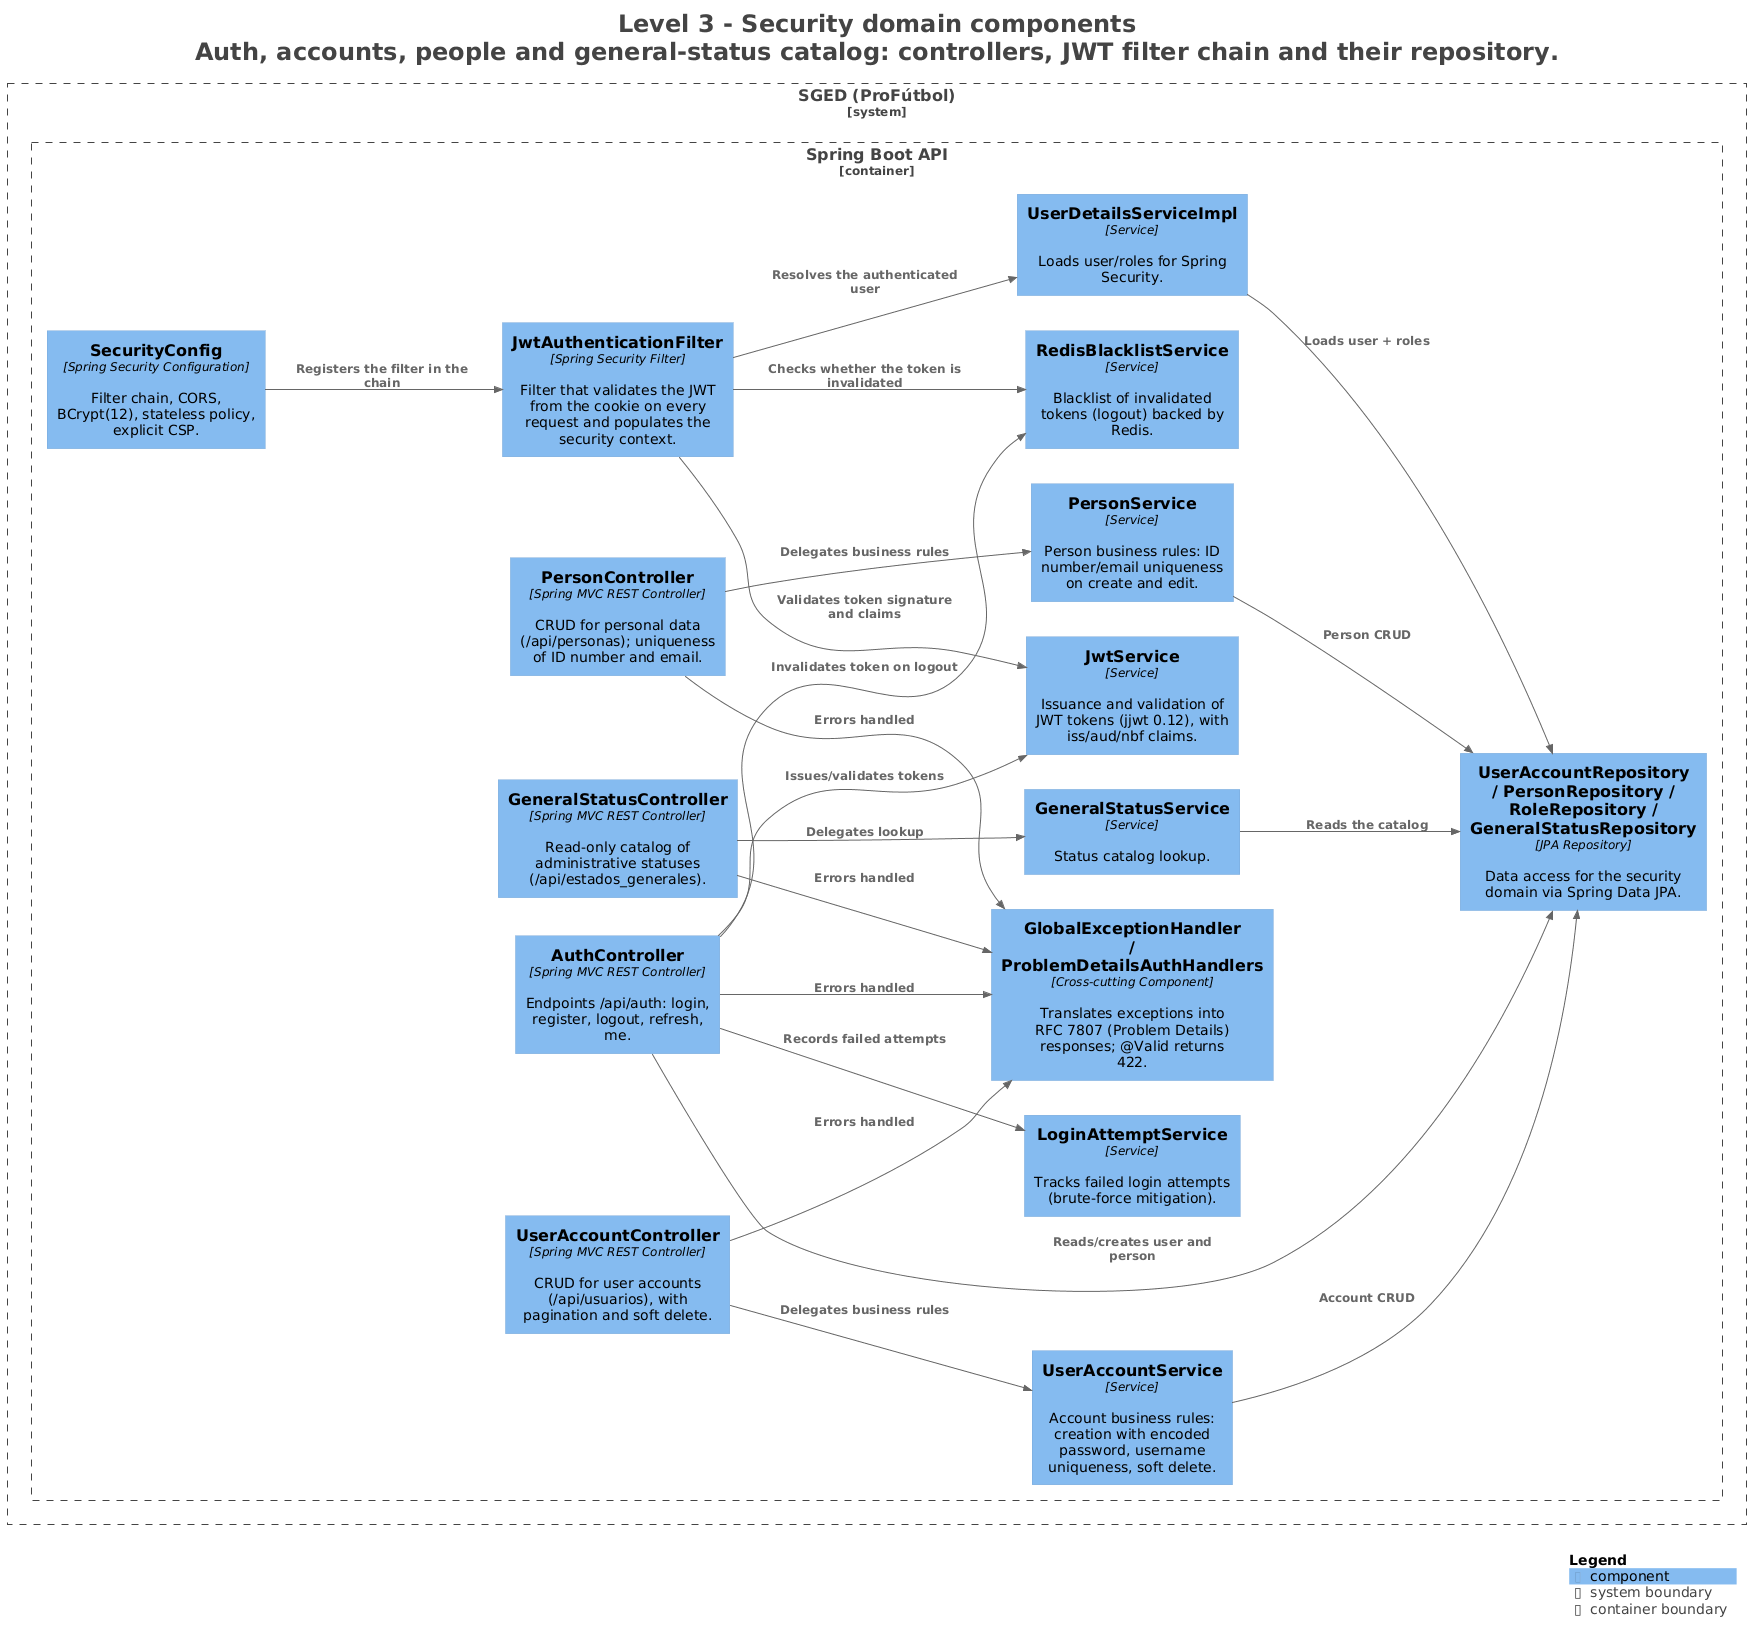
\includegraphics[width=\textwidth]{../arquitectura/L3-seguridad.png}
\caption{C4 nivel 3 — componentes del dominio \texttt{seguridad}, generado desde \ruta{docs/arquitectura/workspace.dsl}.}
\label{fig:c4-l3-seguridad}
\end{figure}

\begin{figure}[htbp]
\centering
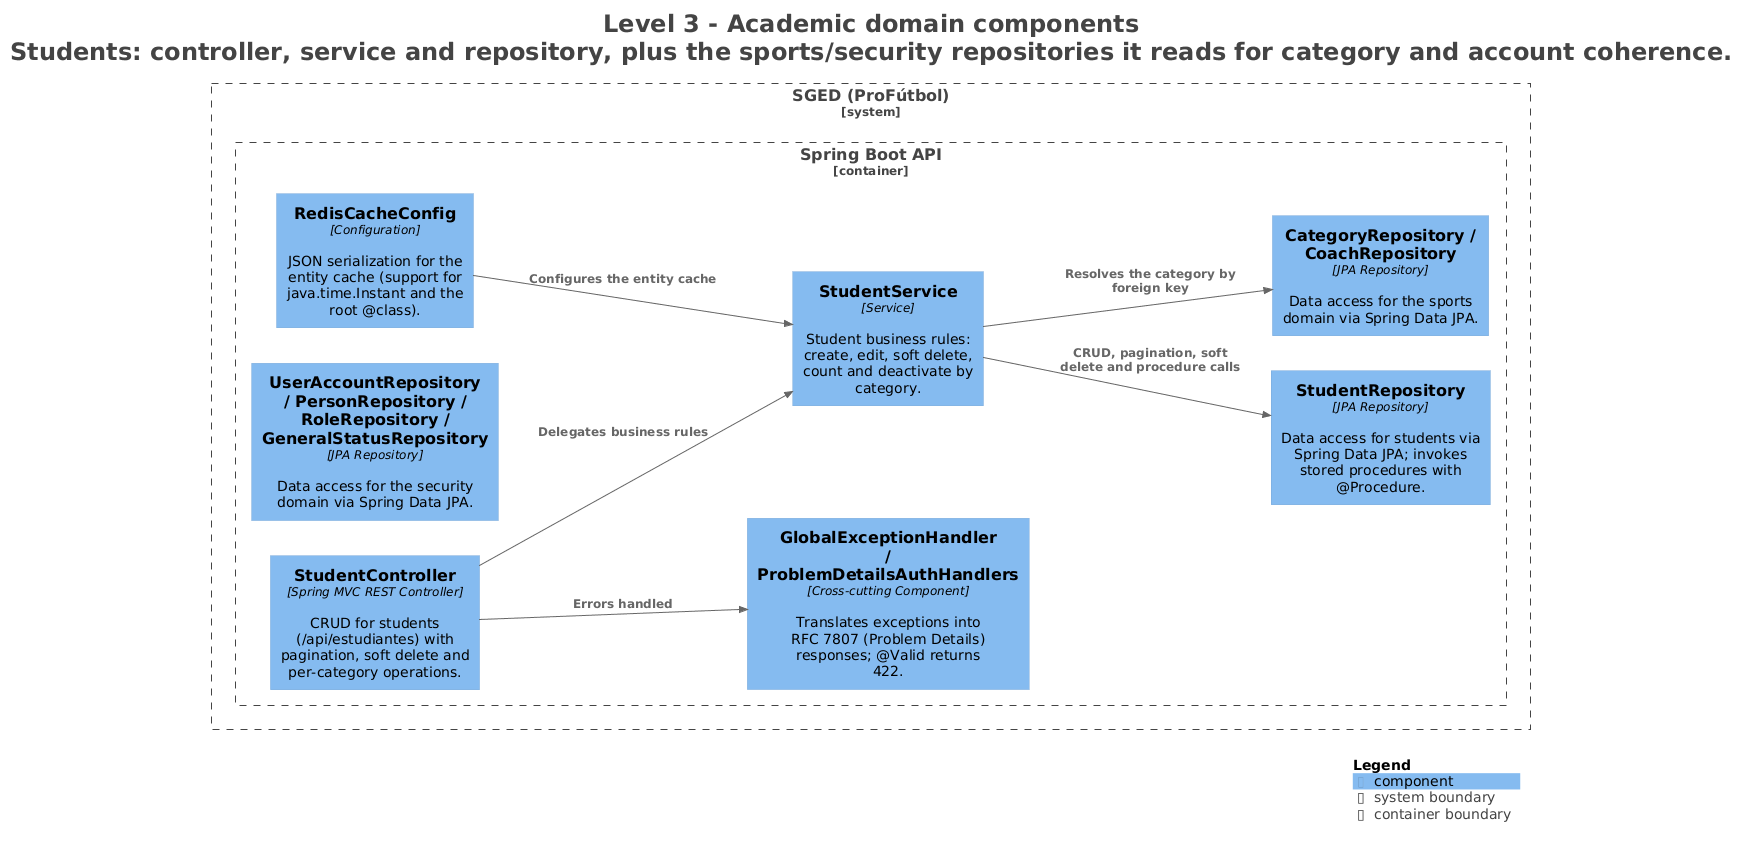
\includegraphics[width=\textwidth]{../arquitectura/L3-academico.png}
\caption{C4 nivel 3 — componentes del dominio \texttt{academico}, generado desde \ruta{docs/arquitectura/workspace.dsl}.}
\label{fig:c4-l3-academico}
\end{figure}

\begin{figure}[htbp]
\centering
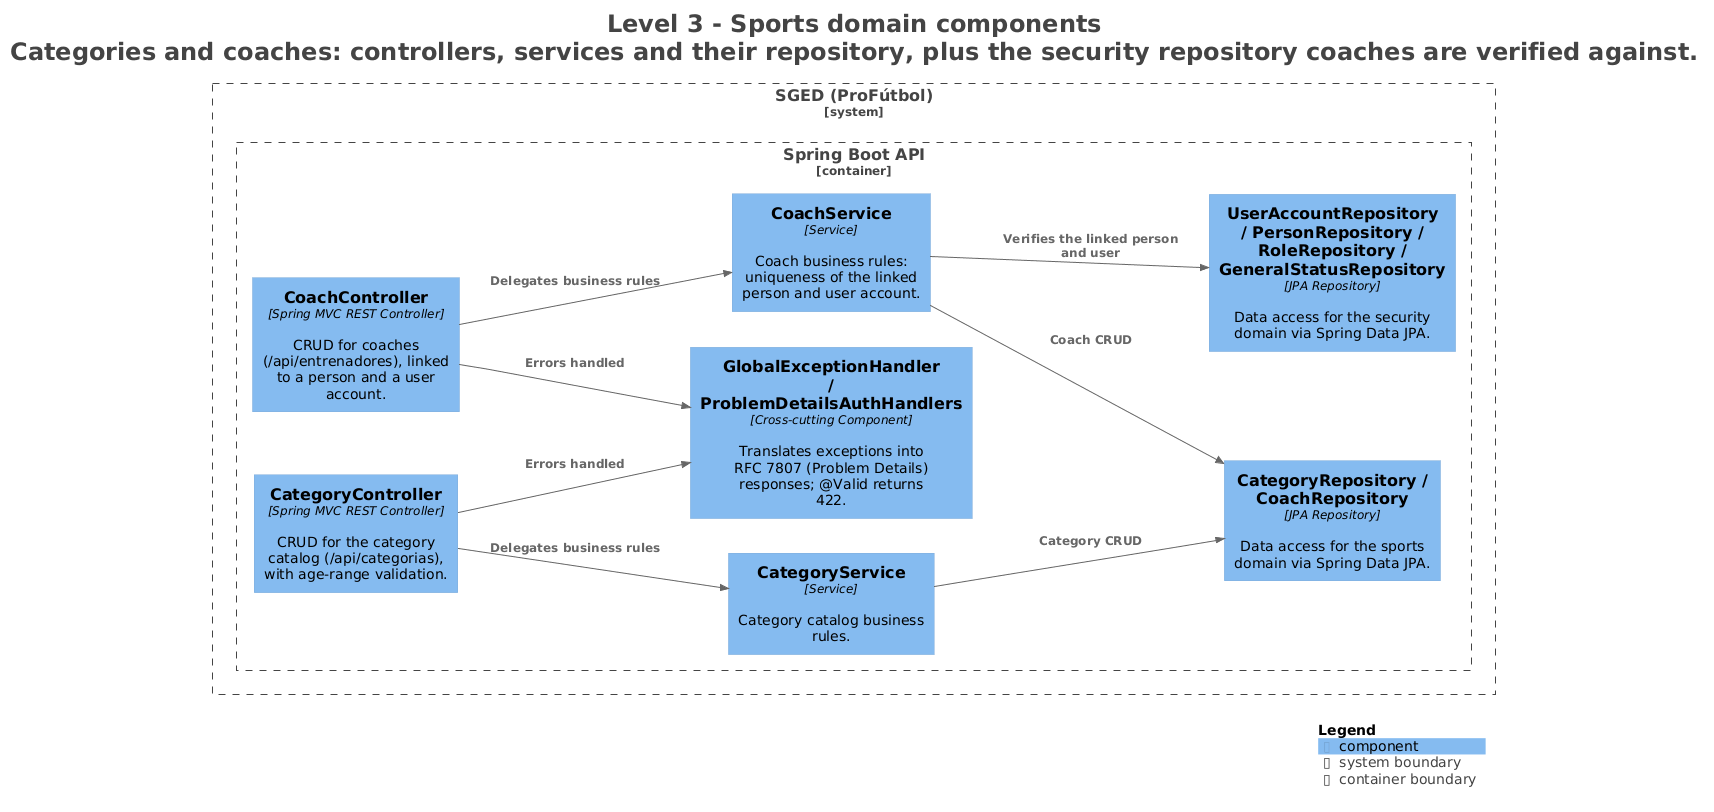
\includegraphics[width=\textwidth]{../arquitectura/L3-deportivo.png}
\caption{C4 nivel 3 — componentes del dominio \texttt{deportivo}, generado desde \ruta{docs/arquitectura/workspace.dsl}.}
\label{fig:c4-l3-deportivo}
\end{figure}

Las tres figuras juntas (\ref{fig:c4-l3-seguridad}--\ref{fig:c4-l3-deportivo})
son la misma vista de componentes que antes se imprimía como un solo
lienzo con los veinte componentes a la vez (\ruta{L3-componentes.png},
que se conserva en el repositorio como referencia, sin imprimirse aquí),
dividida por dominio para que el texto de cada componente sea legible
impreso. Dos detalles merecen lectura
explícita. Primero,
\texttt{StudentRepository} es el único repositorio que invoca
procedimientos almacenados (sección~\ref{sec:acceso-datos}): el resto usa
Spring Data JPA puro, que es exactamente el reparto que exige la estrategia
híbrida. Segundo, \texttt{StudentService} depende del repositorio del
dominio deportivo para resolver la categoría por clave foránea; esa flecha
cruzando de \texttt{academico} a \texttt{deportivo} es la consecuencia
directa de haber normalizado la categoría, y es la clase de acoplamiento
que conviene tener dibujado antes de que crezca.

\subsection{Autenticación: JWT en cookie \texttt{HttpOnly}}
\label{sec:jwt-cookie}

El sistema emite el JWT~\cite{rfc7519} exclusivamente en una cookie
\texttt{HttpOnly}, \texttt{Secure} y \texttt{SameSite=Strict}
(Listado~\ref{lst:cookie-sesion}). El token nunca
viaja en el cuerpo de la respuesta ni se almacena en \texttt{localStorage},
de modo que un ataque de \emph{scripting} entre sitios no puede leerlo.

\begin{lstlisting}[caption={Emisión de la cookie de sesión (\ruta{AuthController.java})},label={lst:cookie-sesion}]
ResponseCookie.from("sged_access", token)
        .httpOnly(true)
        .secure(cookieSecure)
        .sameSite("Strict")
        .path("/")
        .maxAge(Duration.ofMillis(expiracionMs))
        .build();
\end{lstlisting}

Como JWT es \emph{stateless}, cerrar sesión no invalidaría el token por sí
solo. Por eso el sistema mantiene una lista de revocación en Redis indexada
por el identificador del token (\texttt{jti}), con tiempo de vida igual al
tiempo que le restaba al token: un token cerrado deja de ser aceptado
inmediatamente, aunque su firma siga siendo válida.

% ============================================================
\section{Estrategia híbrida de acceso a datos}
\label{sec:acceso-datos}

El Bloque~A.2 de la guía exige una separación explícita entre lo que resuelve
el ORM y lo que debe resolver el motor de base de datos. La regla adoptada
es (Tabla~\ref{tab:reparto-orm-sp}):

\begin{table}[htbp]
\centering
\caption{Reparto de responsabilidades entre ORM y procedimientos almacenados.}
\label{tab:reparto-orm-sp}
\begin{tabular}{@{}p{7.3cm}p{7.3cm}@{}}
\toprule
\textbf{Spring Data JPA (ORM)} & \textbf{Procedimientos almacenados} \\
\midrule
CRUD elemental, consultas paginadas, búsquedas por identificador. &
Agregaciones, actualizaciones masivas con criterio de negocio, operaciones
multi-tabla transaccionales. \\
\bottomrule
\end{tabular}
\end{table}

\textbf{Nota de esta versión del informe:} el sistema creció de dos a
\textbf{siete} procedimientos almacenados desde la Tercera Entrega, uno
por cada categoría funcional que exige el Bloque~A.2.1 de la Entrega
Final. Todos están versionados en \ruta{db/procs/}, creados por
migración Flyway~\cite{flyway} (\texttt{V5}, \texttt{V6}, \texttt{V11},
\texttt{V15}) y catalogados en \ruta{docs/basedatos/CATALOGO-SP.md}, que
es la fuente de verdad que la Tabla~\ref{tab:procs} resume:

\begin{table}[htbp]
\centering
\caption{Procedimientos almacenados de SGED por categoría funcional (Bloque A.2.1).}
\label{tab:procs}
\begin{tabular}{@{}p{4.6cm}p{3.1cm}p{6.2cm}@{}}
\toprule
\textbf{Procedimiento} & \textbf{Categoría} & \textbf{Propósito} \\
\midrule
\texttt{sp\_contar\_estudiantes\_activos} & Cálculo agregado & Conteo de estudiantes activos por categoría \\
\texttt{sp\_desactivar\_estudiantes\_categoria} & Actualización masiva & Baja lógica masiva de una categoría completa \\
\texttt{sp\_validar\_categoria\_estudiante\_sesion} & Validación cruzada & Un estudiante solo marca asistencia en sesiones de su propia categoría \\
\texttt{sp\_generar\_codigo\_estudiante} & Generación de código secuencial & Siguiente \texttt{codigo\_estudiante} consecutivo del año \\
\texttt{sp\_reporte\_asistencia\_estudiante} & Reporte & Porcentaje de asistencia en un rango de fechas \\
\texttt{sp\_contacto\_representante\_estudiante} & Consulta multi-tabla & Contacto de emergencia del representante activo \\
\texttt{sp\_reporte\_stock\_bajo} & Reporte / agregado & Conteo de artículos bajo el mínimo de \emph{stock} \\
\bottomrule
\end{tabular}
\end{table}

\subsection{Un defecto real: \texttt{FUNCTION} frente a \texttt{PROCEDURE}}

La migración \texttt{V5} creó estos objetos como \texttt{FUNCTION}. Al
invocarlos desde Java con \texttt{@Procedure}, Spring Data usa
\texttt{CallableStatement} con sintaxis \texttt{\{call ...\}}, y PostgreSQL
solo acepta \texttt{CALL} contra procedimientos reales~\cite{postgresql16};
el error era explícito: \emph{«... is not a procedure. Hint: To call a
function, use SELECT.»}

La migración \texttt{V6} los convierte en \texttt{PROCEDURE} con parámetro de
salida. Se documenta porque ilustra la diferencia entre «el procedimiento
existe» y «el procedimiento se invoca de verdad»: en la versión anterior el
objeto SQL estaba creado pero quedaba huérfano, y la aplicación seguía
contando en memoria. La invocación correcta
(Listado~\ref{lst:invocacion-sp}):

\begin{lstlisting}[caption={Invocación real desde el repositorio (\ruta{academico/estudiante/repository/EstudianteRepository.java})},label={lst:invocacion-sp}]
@Procedure(procedureName = "academico.sp_contar_estudiantes_activos")
Long contarEstudiantesActivosPorCategoria(@Param("p_categoria") Long idCategoria);
\end{lstlisting}

\emph{Nota sobre esta segunda versión del informe:} el procedimiento se
movió del esquema \texttt{seguridad} a \texttt{academico} y su parámetro
cambió de \texttt{VARCHAR} (nombre de categoría) a \texttt{Long}
(\texttt{id\_categoria}) cuando la categoría se normalizó como entidad
propia — ver sección~\ref{sec:reestructuracion}.

\subsection{Ausencia de SQL dinámico}

Ninguna capa construye sentencias SQL por concatenación de cadenas. Toda
consulta usa parámetros vinculados (JPA) o parámetros nombrados (los
procedimientos). El repositorio incluye una auditoría automatizada
(\ruta{scripts/audit-sql-dynamic.sh}) integrada en \texttt{make audit}.

% ============================================================
\section{Implementación}
\label{sec:implementacion}

Este capítulo describe las decisiones de código que no se derivan
directamente del diagrama de arquitectura (Capítulo~\ref{sec:arquitectura})
ni de la estrategia de acceso a datos (sección~\ref{sec:acceso-datos},
que actúa como la subsección de este capítulo dedicada a esa estrategia,
con su propio listado de código). No se transcriben archivos completos:
cada listado remite al archivo real del repositorio para el detalle.

\subsection{Aislamiento de capas}

La disciplina \emph{controlador~$\rightarrow$~servicio~$\rightarrow$~repositorio}
descrita en la sección~\ref{sec:c4n3} se aplica sin excepción en los 21
controladores del \emph{backend}: ningún controlador inyecta un
repositorio directamente, y ningún repositorio contiene lógica de
negocio. Los cinco dominios (\texttt{seguridad}, \texttt{academico},
\texttt{deportivo}, \texttt{inventario} y el transversal
\texttt{common}) están separados por paquete Java, no solo por
convención de nombres, de modo que un ciclo de dependencias entre
dominios se detecta en tiempo de compilación.

\subsection{Manejo global de errores}

Todas las respuestas de error del \emph{backend} siguen el formato
\emph{Problem Detail} de la RFC~9457~\cite{rfc9457}, centralizado en un
único punto de la capa web (Listado~\ref{lst:exception-handler}):

\begin{lstlisting}[language=Java,caption={Manejador global de excepciones (\ruta{backend/.../common/exception/GlobalExceptionHandler.java})},label={lst:exception-handler}]
@RestControllerAdvice
public class GlobalExceptionHandler {

    @ExceptionHandler(ApiException.class)
    public ProblemDetail handleApiException(ApiException ex) {
        String tipo = ex.getClass().getSimpleName();
        ProblemDetail pd = ex.toProblemDetail(tipo, ex.getStatus().getReasonPhrase());
        pd.setProperty("timestamp", Instant.now().toString());
        return pd;
    }
    // ExceptionHandler adicionales para validacion, autenticacion y autorizacion
}
\end{lstlisting}

Cada excepción de dominio extiende \texttt{ApiException} y declara su
propio código HTTP; el manejador no interpreta tipos de excepción
específicos del dominio, solo los traduce al formato de respuesta
uniforme — la razón por la que agregar un dominio nuevo (representantes,
pagos, inventario) no requirió tocar este archivo.

\subsection{Autenticación en el \emph{frontend}: cookies, no \emph{localStorage}}

El interceptor HTTP de Angular no lee ni adjunta el JWT manualmente — es
la cookie \texttt{HttpOnly} (sección~\ref{sec:jwt-cookie}) la que viaja
automáticamente con cada petición del mismo origen
(Listado~\ref{lst:auth-interceptor}):

\begin{lstlisting}[caption={Interceptor de autenticación (\ruta{frontend/src/app/auth/auth.interceptor.ts})},label={lst:auth-interceptor}]
export const authInterceptor: HttpInterceptorFn = (req, next) => {
  return next(req.clone({ withCredentials: true }));
};
\end{lstlisting}

La brevedad del interceptor es intencional y es la consecuencia directa
de la decisión de \texttt{ADR-002}/\texttt{ADR-008}: al no poder leer la
cookie desde JavaScript, el \emph{frontend} no tiene lógica de adjuntar
ni refrescar el token por su cuenta — delega esa responsabilidad
enteramente en el navegador y en el filtro de seguridad del
\emph{backend}.

\subsection{Caché de consultas de listado}
\label{sec:cache-adr}

El \texttt{ADR-005} (\ruta{docs/adr/ADR-005-cache.md}) fija Redis como caché de consultas, y el
\emph{backend} anota con \texttt{@Cacheable} los tres servicios de
listado de mayor lectura (\texttt{Student}, \texttt{Trainer} y
\texttt{UserAccount}). Durante la preparación de la defensa se detectó
que las anotaciones existían pero la caché nunca llegó a estar
operativa: faltaba \texttt{@EnableCaching}, de modo que cada petición
consultaba PostgreSQL aunque Redis estuviera sembrado. El defecto se
corrigió en dos archivos: \ruta{backend/.../BackendApplication.java}
activa el soporte declarativo, y \ruta{backend/.../config/RedisCacheConfig.java}
configura el serializador con \emph{polymorphic typing} explícito
(tipos de datos registrados con \texttt{BasicPolymorphicTypeValidator}),
sin el cual las respuestas cacheadas comienzan a devolverse como
\texttt{LinkedHashMap} y rompen el contrato de tipos del \emph{endpoint}
—un defecto que las mediciones de la sección~\ref{sec:rendimiento}
documentan como resuelto. La caché quedó verificada en caliente: la
primera petición (fría, sin clave) tarda $\approx$270--300\,ms; la
segunda (misma clave) cae a $\approx$75--105\,ms y genera la clave
\texttt{estudiantes::0-10} en Redis.

\subsection{Configuración por entorno}

La configuración de Spring Boot vive en un único \ruta{application.yml}
con valores parametrizados por variable de entorno (\ruta{.env.example}
documenta cada una sin valores sensibles); no existen perfiles
\texttt{application-\{dev,prod\}.yml} duplicados que puedan divergir
entre sí. En \ruta{docker-compose.yml} las imágenes de PostgreSQL y
Redis están fijadas por \emph{digest} \texttt{sha256} en vez de por
etiqueta \texttt{latest}, para que \texttt{make up} reproduzca el mismo
binario en cualquier máquina (Bloque~D.2).

% ============================================================
\section{Requisitos y modelo de datos}
\label{sec:requisitos}

\subsection{Resumen de requisitos}

La especificación completa está en \ruta{docs/requisitos/SRS.md}. Se resumen
aquí los requisitos funcionales con su estado real y el \emph{endpoint} o
esquema que los materializa.

\renewcommand{\arraystretch}{1.15}
\begin{longtable}{@{}p{1.3cm}p{7.4cm}p{4.6cm}p{1.7cm}@{}}
\toprule
\textbf{ID} & \textbf{Requisito} & \textbf{Implementación} & \textbf{Estado} \\
\midrule
\endfirsthead
\toprule
\textbf{ID} & \textbf{Requisito} & \textbf{Implementación} & \textbf{Estado} \\
\midrule
\endhead

RF-01 & Registro de usuarios por administrador & \texttt{POST /api/auth/registro} & \ok \\
RF-02 & Autenticación con JWT en cookie \texttt{HttpOnly} & \texttt{POST /api/auth/login} & \ok \\
RF-03 & Cierre de sesión con revocación efectiva por \texttt{jti} & \texttt{POST /api/auth/logout} & \ok \\
RF-04 & Renovación de sesión sin re-credenciales & \texttt{POST /api/auth/refresh} & \ok \\
RF-05 & Consulta de la sesión activa & \texttt{GET /api/auth/me} & \ok \\
RF-06 & Bloqueo tras 5 intentos fallidos en 15 minutos & \texttt{LoginAttemptService} & \ok \\
RF-07 & Comprobación de disponibilidad & \texttt{GET /api/auth/ping} & \ok \\
RF-08 & Listado paginado de estudiantes & \texttt{GET /api/estudiantes} & \ok \\
RF-09 & Consulta por identificador con \texttt{404} tipificado & \texttt{GET /api/estudiantes/\{id\}} & \ok \\
RF-10 & Registro transaccional de estudiante & \texttt{POST /api/estudiantes} & \ok \\
RF-11 & Validación del formato de categoría (\texttt{SUB-NN}) & \texttt{EstudianteRequest} & \ok \\
RF-12 & Actualización de estudiante & \texttt{PUT /api/estudiantes/\{id\}} & \ok \\
RF-13 & Baja lógica preservando el historial & \texttt{DELETE /api/estudiantes/\{id\}} & \ok \\
RF-14 & Conteo de activos por categoría (en el motor) & \texttt{sp\_contar\_estudiantes\_activos} & \ok \\
RF-15 & Desactivación masiva por categoría (en el motor) & \texttt{sp\_desactivar\_estudiantes\_categoria} & \ok \\
\midrule
RF-16 & Gestión de entrenadores & \texttt{deportivo.entrenadores} & Modelado \\
RF-17 & Horarios recurrentes de entrenamiento & \texttt{horarios\_entrenamiento} & Modelado \\
RF-18 & Sesiones de entrenamiento con ciclo de estados & \texttt{sesiones\_entrenamiento} & Modelado \\
RF-19 & Asistencia por RFID o manual & \texttt{deportivo.asistencias} & Modelado \\
RF-20 & Evaluación diaria por criterios & \texttt{detalle\_evaluacion} & Modelado \\
RF-21 & Promedios de evaluación & \texttt{v\_promedio\_evaluacion} & Modelado \\
RF-22 & Notificación a representantes & --- & Planificado \\
\bottomrule
\end{longtable}
\renewcommand{\arraystretch}{1}

Los requisitos no funcionales (RNF-01 a RNF-13) se verifican con las
mediciones de la sección siguiente. La matriz
\ruta{docs/trazabilidad/matriz.csv} enlaza cada uno con su prueba y su
evidencia.

\subsection{Catálogo de la API REST}
\label{sec:catalogo-api}

La superficie expuesta es de siete recursos y treinta \emph{endpoints}. Se
lista completa porque es la forma más directa de contrastar lo que el
sistema realmente ofrece contra lo que los requisitos declaran, y porque la
columna de autorización es la que concentró el defecto de la
sección~\ref{sec:a01-falso-correcto}. \textsc{a} abrevia
\textsc{administrador}; \textsc{e}, \textsc{entrenador}; \textsc{u}, el rol
\textsc{user}.

\renewcommand{\arraystretch}{1.15}
\begin{longtable}{@{}llll@{}}
\toprule
\textbf{Método y ruta} & \textbf{Operación} & \textbf{Roles} & \textbf{RF} \\
\midrule
\endhead
\multicolumn{4}{@{}l}{\textit{Autenticación} — \texttt{/api/auth}} \\
\midrule
\texttt{POST /login} & Inicia sesión, emite cookies & Público & RF-02 \\
\texttt{POST /registro} & Alta de cuenta & \textsc{a} & RF-01 \\
\texttt{POST /logout} & Revoca el token en Redis & Autenticado & RF-03 \\
\texttt{POST /refresh} & Renueva el \emph{access token} & Autenticado & RF-04 \\
\texttt{GET /me} & Datos de la sesión actual & Autenticado & RF-05 \\
\texttt{GET /ping} & Sonda de disponibilidad & Público & --- \\
\midrule
\multicolumn{4}{@{}l}{\textit{Estudiantes} — \texttt{/api/estudiantes}} \\
\midrule
\texttt{GET /} & Listado paginado y ordenable & \textsc{a e u} & RF-08 \\
\texttt{GET /\{id\}} & Consulta individual & \textsc{a e u} & RF-09 \\
\texttt{POST /} & Alta & \textsc{a} & RF-10 \\
\texttt{PUT /\{id\}} & Edición & \textsc{a} & RF-12 \\
\texttt{DELETE /\{id\}} & Baja lógica & \textsc{a} & RF-13 \\
\texttt{GET /conteo/categoria/\{id\}} & Conteo por procedimiento & \textsc{a e} & RF-14 \\
\texttt{POST /operaciones/} & Desactivación masiva por & \textsc{a} & RF-15 \\
\quad\texttt{desactivar-categoria} & \quad procedimiento & & \\
\midrule
\multicolumn{4}{@{}l}{\textit{Categorías} — \texttt{/api/categorias}} \\
\midrule
\texttt{GET /} & Listado paginado & \textsc{a e u} & RF-23 \\
\texttt{GET /activas} & Catálogo para formularios & \textsc{a e u} & RF-23 \\
\texttt{GET /\{id\}} & Consulta individual & \textsc{a e u} & RF-23 \\
\texttt{POST /} & Alta con rango de edad & \textsc{a} & RF-23 \\
\texttt{PUT /\{id\}} & Edición & \textsc{a} & RF-23 \\
\texttt{DELETE /\{id\}} & Baja lógica & \textsc{a} & RF-23 \\
\midrule
\multicolumn{4}{@{}l}{\textit{Entrenadores} — \texttt{/api/entrenadores}} \\
\midrule
\texttt{GET /} & Listado paginado & \textsc{a e} & RF-24 \\
\texttt{GET /\{id\}} & Consulta individual & \textsc{a e} & RF-24 \\
\texttt{POST /} & Alta con persona y cuenta & \textsc{a} & RF-24 \\
\texttt{PUT /\{id\}} & Edición & \textsc{a} & RF-24 \\
\texttt{DELETE /\{id\}} & Baja lógica & \textsc{a} & RF-24 \\
\midrule
\multicolumn{4}{@{}l}{\textit{Personas} — \texttt{/api/personas} \quad\small(datos identificativos de menores)} \\
\midrule
\texttt{GET /} & Listado paginado & \textsc{a} & RF-25 \\
\texttt{GET /\{id\}} & Consulta individual & \textsc{a} & RF-25 \\
\texttt{GET /cedula/\{cedula\}} & Búsqueda por cédula & \textsc{a} & RF-25 \\
\texttt{POST /} & Alta & \textsc{a} & RF-25 \\
\texttt{PUT /\{id\}} & Edición & \textsc{a} & RF-25 \\
\texttt{DELETE /\{id\}} & Baja lógica & \textsc{a} & RF-25 \\
\midrule
\multicolumn{4}{@{}l}{\textit{Usuarios y catálogos}} \\
\midrule
\texttt{/api/usuarios} (5 verbos) & CRUD de cuentas & \textsc{a} & RF-26 \\
\texttt{GET /api/estados\_generales} & Catálogo de estados & \textsc{a e u} & RF-26 \\
\bottomrule
\end{longtable}
\renewcommand{\arraystretch}{1}

Dos observaciones que la tabla hace evidentes. La primera es que
\texttt{/api/personas} es el recurso con la superficie más sensible del
sistema —seis \emph{endpoints} sobre datos identificativos de menores,
incluido uno de búsqueda directa por cédula— y es exactamente el que
estuvo sin control de acceso. La segunda es que el dominio deportivo
expuesto se limita hoy a categorías y entrenadores: horarios, sesiones,
asistencias y evaluaciones tienen esquema en la base de datos pero ninguna
ruta REST, y son el objetivo declarado de la Entrega Final.

\subsection{Modelo de datos}

El esquema se divide en dos espacios de nombres con responsabilidades
separadas (Tabla~\ref{tab:esquemas}):

\begin{table}[htbp]
\centering
\caption{Esquemas del modelo de datos de SGED.}
\label{tab:esquemas}
\begin{tabular}{@{}llp{7.4cm}@{}}
\toprule
\textbf{Esquema} & \textbf{Tablas} & \textbf{Contenido} \\
\midrule
\texttt{seguridad} & 6 & Personas, usuarios, roles, relación usuario-rol,
estados y estudiantes. \\
\texttt{deportivo} & 9 & Posiciones, entrenadores, horarios, sesiones,
asistencias, criterios, evaluaciones, detalle y observaciones. \\
\bottomrule
\end{tabular}
\end{table}

Decisiones de modelado relevantes, todas materializadas como restricciones
en el motor y no solo como validación en la aplicación:

\begin{itemize}[leftmargin=*]
  \item \textbf{Baja lógica en lugar de borrado.} Las asistencias y
    evaluaciones referencian al estudiante por clave foránea; borrarlo
    físicamente destruiría su historial deportivo.
  \item \textbf{Unicidad parcial del código RFID.}
    \texttt{UNIQUE \ldots WHERE rfid\_codigo IS NOT NULL} permite muchos
    estudiantes sin credencial, pero impide que dos compartan la misma.
  \item \textbf{Una asistencia por sesión y estudiante.}
    \texttt{UNIQUE (id\_sesion, id\_estudiante)}.
  \item \textbf{Posición jugada por evaluación.}
    \texttt{detalle\_evaluacion} guarda la posición de \emph{ese} día,
    distinta de la habitual del estudiante, para que el histórico quede
    correctamente etiquetado cuando alguien juega fuera de su posición.
  \item \textbf{Coherencia temporal.}
    \texttt{CHECK (hora\_fin > hora\_inicio)} y
    \texttt{CHECK (dia\_semana BETWEEN 1 AND 7)} en los horarios.
\end{itemize}

El diccionario completo, con tipos, restricciones y disparadores, está en
\ruta{docs/basedatos/DATA-DICTIONARY.md}. El esquema no lo genera el ORM:
\texttt{ddl-auto} está fijado en \texttt{validate}, de modo que la aplicación
falla al arrancar si el esquema real y las entidades divergen.

% ============================================================
\section{Materiales y métodos}
\label{sec:protocolo}

Todas las mediciones de este informe se generaron ejecutando el sistema real
levantado con \texttt{make up}, no en simulación, y sus artefactos crudos
están versionados sin edición manual. Este capítulo declara el enfoque
metodológico (sección~\ref{sec:dsr}), los instrumentos
(sección~\ref{sec:instrumentos}) y el procedimiento antes de presentar los
resultados (Capítulo~\ref{sec:evaluacion}), para que un tercero pueda
repetirlos y obtener cifras comparables.

\subsection{Enfoque metodológico}
\label{sec:dsr}

El trabajo sigue \emph{Design Science Research} (DSR) en la formulación de
Peffers~\emph{et al.}~\cite{peffers2007}, articulada con los criterios de
rigor y relevancia de Hevner~\emph{et al.}~\cite{hevner2004} —un marco que
la revisión de Engström~\emph{et al.} confirma como infrecuente en la
investigación de ingeniería de software pese a encajar naturalmente con
ella, precisamente porque buena parte de esa investigación ya diseña
soluciones a problemas prácticos sin nombrar explícitamente el
paradigma~\cite{engstrom2020dsr}—, en sus seis
actividades:

\begin{enumerate}[leftmargin=*]
  \item \textbf{Identificación del problema y motivación} —
    sección~\ref{sec:contexto-motivacion}: gestión administrativa y
    deportiva fragmentada, sin trazabilidad ni control de acceso sobre
    datos de menores.
  \item \textbf{Definición de objetivos de una solución} —
    sección~\ref{sec:objetivos}: objetivo general y cinco objetivos
    específicos trazados a las cuatro preguntas de investigación.
  \item \textbf{Diseño y desarrollo} — Capítulo~\ref{sec:arquitectura} y
    sección~\ref{sec:acceso-datos}: arquitectura en C4, estrategia
    híbrida de acceso a datos, ocho ADR.
  \item \textbf{Demostración} — el sistema desplegado y operable
    (\texttt{make up}), con datos sembrados y los cinco roles de usuario
    reales.
  \item \textbf{Evaluación} — Capítulo~\ref{sec:evaluacion}: contraste
    empírico contra los umbrales de rendimiento, seguridad, cobertura,
    calidad web y usabilidad declarados en este capítulo.
  \item \textbf{Comunicación} — este documento, el repositorio público y
    la defensa oral del PFC.
\end{enumerate}

El ciclo no fue lineal: la Tercera Entrega ya había ejecutado una vuelta
completa de demostración y evaluación, y esta entrega repite las
actividades 3 a 5 sobre el sistema ampliado, en la lógica iterativa que
el propio modelo de Peffers admite entre sus actividades.

\subsection{Instrumentos de medición}
\label{sec:instrumentos}

La Tabla~\ref{tab:instrumentos} enumera el instrumento y la
configuración exacta usados en cada bloque de evaluación.

\begin{table}[htbp]
\centering
\caption{Instrumentos de medición usados en la evaluación empírica.}
\label{tab:instrumentos}
\begin{tabular}{@{}llp{7cm}@{}}
\toprule
\textbf{Bloque} & \textbf{Instrumento} & \textbf{Configuración} \\
\midrule
Rendimiento & k6 & \ruta{k6/listado-estudiantes.js}, 50 VU, 30\,s, umbrales declarados en el propio \emph{script} \\
Seguridad & \texttt{curl} + análisis estático & \ruta{scripts/audit-owasp.sh}, \ruta{scripts/audit-sql-dynamic.sh} \\
Cobertura & JaCoCo & Umbral 70\,\% líneas y \emph{branches}, configurado en \ruta{backend/pom.xml} \\
Calidad web & Lighthouse & \ruta{lighthouserc.js} \\
Usabilidad & SUS (Brooke) & Cuestionario de 10 ítems sin modificación~\cite{brooke1996}, escala adjetival de Bangor~\emph{et al.}~\cite{bangor2009} \\
\bottomrule
\end{tabular}
\end{table}

\subsection{Enfoque de métricas: un GQM completo}
\label{sec:gqm}

Las métricas del sistema se alinean con el marco \emph{Goal-Question-Metric}
de Basili~\emph{et al.}~\cite{basili1994gqm}. Se presenta un GQM completo
(Tabla~\ref{tab:gqm}), correspondiente a RQ1 (sección~\ref{sec:rqs}):

\begin{table}[htbp]
\centering
\caption{Ejemplo de Goal-Question-Metric para RQ1.}
\label{tab:gqm}
\begin{tabular}{@{}p{2.4cm}p{12cm}@{}}
\toprule
\textbf{Meta (\emph{Goal})} & Caracterizar el rendimiento del \emph{endpoint} de listado protegido bajo carga concurrente, desde el punto de vista del equipo de desarrollo, en el contexto del ambiente de pruebas de la Entrega Final. \\
\textbf{Pregunta 1} & ¿Cuál es la latencia p95 del \emph{endpoint} bajo 50 usuarios virtuales concurrentes? \\
\textbf{Métrica 1} & p95 de tiempo de respuesta (ms), agregado sobre corridas independientes, con intervalo de confianza al 95\,\%. \\
\textbf{Pregunta 2} & ¿El sistema devuelve errores de servidor bajo esa carga? \\
\textbf{Métrica 2} & Tasa de respuestas HTTP $\geq$ 500 sobre el total de peticiones de la corrida. \\
\bottomrule
\end{tabular}
\end{table}

\subsection{Población, muestreo y participantes}
\label{sec:muestreo}

Para la componente de usabilidad, la población objetivo son los cinco
perfiles de usuario reales del sistema (administrador, entrenador,
recepcionista, estudiante, representante). El muestreo fue por
conveniencia —participantes disponibles del entorno cercano al
equipo—, siguiendo la clasificación de técnicas de muestreo de Baltes y
Ralph~\cite{baltesralph2022}, quienes documentan que es la técnica más
frecuente y a la vez la que exige declarar sus límites en vez de
omitirlos. \textbf{Limitación declarada:} $N=15$ es una muestra pequeña
y no probabilística; los resultados por perfil (tres o cuatro
participantes por rol) se interpretan como indicativos de un patrón, no
como una estimación poblacional generalizable —la razón por la que
sección~\ref{sec:sus} reporta el desglose por perfil en vez de solo la
media agregada.

\textbf{Recolección en dos fases.} Los diez primeros cuestionarios se
aplicaron el 30 de julio de 2026 y los cinco restantes el 18 de agosto,
para alcanzar el mínimo de quince que exige la Entrega Final. Se declara
explícitamente porque afecta a cómo debe leerse el dato: la segunda
tanda se recogió sobre una versión posterior del sistema, de modo que
los quince cuestionarios no evalúan exactamente el mismo artefacto. El
efecto sobre el agregado fue pequeño y se documenta en
\ruta{docs/mediciones/sus/INTERPRETACION.md}: la media se movió 1{,}08
puntos (68{,}25 a 69{,}33) mientras el intervalo de confianza se
estrechó en torno a un tercio, lo que sugiere que la ampliación precisó
la estimación sin desplazarla.

\textbf{Numeración.} Los identificadores van de ENC-01 a ENC-10 y de
ENC-13 a ENC-17: no existen ENC-11 ni ENC-12. El salto se conserva tal
como llegaron los datos en vez de renumerar, para no presentar como
serie continua una que no lo es.

\subsection{Análisis estadístico declarado a priori}
\label{sec:analisis-estadistico}

Antes de ejecutar las mediciones se fijaron los estadísticos a reportar:
media, mediana, desviación típica e intervalo de confianza al 95\,\%
para todas las métricas cuantitativas; percentiles p50, p90 y p95 para
rendimiento. Se prefieren intervalos de confianza sobre valores~$p$ como
forma primaria de reporte, siguiendo la recomendación del Bloque~C de la
guía. Las cinco corridas independientes de k6 por escenario que exige el
Bloque~A.1 están archivadas en \ruta{docs/mediciones/perf/}; el escenario
de caché cálida mide el \emph{endpoint} con la página de consulta ya
resuelta por Redis, y el de caché fría barre páginas distintas con la
caché vacía para forzar \emph{misses} reales contra el volumen de datos.

La comparación entre escenarios es un contraste inferencial no paramétrico
con tamaño de efecto y corrección por comparaciones múltiples, conforme al
Bloque~C de la guía: test de Mann-Whitney (Wilcoxon) bilateral, estadístico
A12 de Vargha y Delaney~\cite{varghadelaney2000} y delta de
Cliff~\cite{cliff1993} para procesos ordinales, y corrección de
Holm-Bonferroni~\cite{holm1979} sobre las comparaciones emparejadas
corrida-a-corrida (sección~\ref{sec:rendimiento}). En el desglose de
usabilidad por perfil no hay contraste entre grupos —3 o 4 participantes
por perfil no lo soportan—, por lo que la corrección múltiple se aplica
exclusivamente al rendimiento (sección~\ref{sec:analisis-estadistico}).

\subsection{Entorno de ejecución}
\label{sec:entorno}

La Tabla~\ref{tab:entorno} fija el entorno exacto en el que se
generaron todas las mediciones de este capítulo.

\begin{table}[htbp]
\centering
\caption{Entorno de ejecución de las mediciones.}
\label{tab:entorno}
\begin{tabular}{@{}lp{9.2cm}@{}}
\toprule
\textbf{Elemento} & \textbf{Valor} \\
\midrule
Anfitrión & Linux (x86\_64), Docker Engine en contenedores \\
Contenedores & \texttt{postgres} y \texttt{redis} fijados por digest \texttt{sha256} en \texttt{docker-compose.yml}; backend y frontend construidos desde el repositorio \\
Backend & Spring Boot 3.2.5 sobre Temurin JDK 21 \\
Estado inicial & Base de datos creada desde cero (\texttt{docker compose down -v}) y sembrada con \ruta{db/seed.sql} y el volumen sintético \ruta{db/carga-volumen.sql} (2401 estudiantes activos) \\
Red & Todas las peticiones contra \texttt{localhost}; sin latencia de red externa \\
\bottomrule
\end{tabular}
\end{table}

El estado inicial no es un detalle menor. Los \emph{scripts} de
inicialización de PostgreSQL solo se ejecutan cuando el directorio de datos
está vacío: al reutilizar un volumen anterior, el esquema queda congelado en
una versión previa y el \emph{backend} no arranca. Toda medición reportada
aquí parte de volumen limpio.

\subsection{Procedimiento por bloque}

La Tabla~\ref{tab:procedimiento-bloque} detalla, para cada bloque del
enfoque GQM (sección~\ref{sec:gqm}), la herramienta y el procedimiento
de control de variabilidad aplicados.

\begin{table}[htbp]
\centering
\caption{Procedimiento de medición por bloque de evaluación.}
\label{tab:procedimiento-bloque}
\begin{tabular}{@{}llp{6.1cm}@{}}
\toprule
\textbf{Bloque} & \textbf{Herramienta} & \textbf{Procedimiento y control de variabilidad} \\
\midrule
C.1 Rendimiento & k6 & \texttt{make bench}: 5 corridas independientes de 50 usuarios virtuales durante 30\,s por escenario (caché cálida y caché fría). Se reportan media, p90, p95 e intervalo de confianza al 95\,\% sobre las corridas, no una sola. \\
C.2/C.4 Seguridad & \texttt{curl} & \texttt{make audit}: peticiones reales contra el sistema en ejecución, guardando la respuesta HTTP íntegra con cabeceras. Cada control se contrasta en sus dos direcciones: lo que debe rechazarse y lo que debe seguir permitido. \\
C.3 Usabilidad & SUS en papel & Cuestionario de Brooke de 10 ítems aplicado a 15 participantes externos en dos tandas; transcripción a CSV y cálculo con \ruta{scripts/sus-analysis.py}, cuya aritmética se validó contra los cuatro casos de referencia de la literatura (0, 50, 75 y 100 puntos). \\
Cobertura & JaCoCo & \texttt{make test}, que ejecuta \texttt{clean test} para que la instrumentación no alcance clases de compilaciones anteriores. \\
C.5 Accesibilidad & Lighthouse & 3 corridas mediante \ruta{lighthouserc.js}; se reportan los cuatro puntajes agregados y las métricas Web Vitals. \\
\bottomrule
\end{tabular}
\end{table}

\subsection{Determinismo, semillas y trazabilidad}

Los archivos crudos (\texttt{.json} de k6 y Lighthouse, \texttt{.txt} de las
respuestas HTTP, \texttt{.csv} del SUS y de JaCoCo) se conservan tal como los
produjo cada herramienta; los reportes en Markdown se generan a partir de
ellos mediante los \emph{scripts} de \ruta{scripts/}, nunca a mano. Cada
archivo de evidencia lleva en su cabecera la fecha en UTC, el \emph{commit}
corto y la versión de la herramienta que lo generó, de modo que una cifra del
informe pueda rastrearse hasta la ejecución concreta que la produjo.

\ruta{scripts/perf-analysis.py} fija semilla aleatoria \texttt{42} para
cualquier remuestreo estadístico sobre los datos crudos de k6, declarada
en la cabecera del propio \emph{script} y en \ruta{docs/mediciones/perf/REPORT.md}.
Los datos de SUS y de JaCoCo no requieren semilla porque no involucran
muestreo aleatorio: son transcripción directa (SUS) o instrumentación
determinista de cobertura (JaCoCo). Las versiones exactas de cada
herramienta (k6, Lighthouse, JDK, Docker) se declaran por corrida en
\ruta{docs/entorno/versions.txt} y en la cabecera de cada archivo crudo.

% ============================================================
\section{Evidencia empírica}
\label{sec:evaluacion}

\subsection{Rendimiento (Bloque C.1)}
\label{sec:rendimiento}

Diez corridas independientes de k6, cinco por escenario, con 50 usuarios
virtuales durante 30 segundos contra el \emph{endpoint} protegido
\texttt{GET /api/estudiantes} — cumple el mínimo de cinco corridas por
escenario que exige la guía. El escenario de caché cálida consulta
siempre la misma página (\texttt{page=0}) ya resuelta por Redis; el de
caché fría barre las 241 páginas de los 2401 estudiantes activos
sembrados con \ruta{db/carga-volumen.sql}, con la caché vaciada
(\texttt{FLUSHALL}) antes de cada corrida, de modo que cada primera
visita a una página cae a PostgreSQL (un \emph{miss} real). Las corridas
se regeneraron el 2026-09-07 contra el sistema local completo sobre el
\emph{commit} defendido, tras corregir el defecto de \ruta{.env}
descrito en la sección~\ref{sec:estado-entrega} y activar la caché de
Redis que la sección~\ref{sec:cache-adr} documenta.

La decisión de repetir la medición y reportar un intervalo de confianza,
en vez de publicar el resultado de una sola corrida, sigue el argumento
metodológico de Georges~\emph{et al.}: una única ejecución de un sistema
sobre JVM no caracteriza su rendimiento, porque la variación entre
corridas puede ser del mismo orden que la diferencia que se pretende
reportar, y sin estadística de intervalos no hay forma de distinguir una
de otra~\cite{georges2007benchmarking}. Los resultados: no

\begin{table}[htbp]
\centering
\caption{Caché cálida: resultados de las corridas de rendimiento (k6, \ruta{docs/mediciones/perf/k6-run*.json}).}
\label{tab:k6-resultados}
\begin{tabular}{@{}lrrrrrrr@{}}
\toprule
\textbf{Corrida} & \textbf{Media (ms)} & \textbf{Mediana} & \textbf{p90} & \textbf{p95} & \textbf{p99} & \textbf{Errores} & \textbf{RPS} \\
\midrule
1 (calentamiento) & 56,66 & 45,56 & 104,87 & 137,08 & 204,28 & 0,00\,\% & 273,55 \\
2 & 15,63 & 12,78 & 26,34 & 32,50 & 49,76 & 0,00\,\% & 370,96 \\
3 & 10,33 & 9,22  & 14,56 & 17,40 & 25,44 & 0,00\,\% & 389,64 \\
4 & 9,33  & 8,75  & 12,07 & 13,99 & 20,05 & 0,00\,\% & 393,48 \\
5 & 9,83  & 9,01  & 13,20 & 15,88 & 22,15 & 0,00\,\% & 390,28 \\
\midrule
\textbf{Agregado 2--5} & \textbf{11,28} & --- & --- & \textbf{19,94} & \textbf{29,35} & --- & \textbf{386,09} \\
\bottomrule
\end{tabular}
\end{table}

\begin{table}[htbp]
\centering
\caption{Caché fría: resultados de las corridas de rendimiento (k6, \ruta{docs/mediciones/perf/k6-frio*.json}).}
\label{tab:k6-resultados-frio}
\begin{tabular}{@{}lrrrrrrr@{}}
\toprule
\textbf{Corrida} & \textbf{Media (ms)} & \textbf{Mediana} & \textbf{p90} & \textbf{p95} & \textbf{p99} & \textbf{Errores} & \textbf{RPS} \\
\midrule
1 & 20,39 & 18,54 & 36,02 & 41,72 & 52,53 & 0,00\,\% & 356,15 \\
2 & 18,81 & 15,92 & 34,14 & 39,77 & 50,89 & 0,00\,\% & 361,16 \\
3 & 16,49 & 11,45 & 32,06 & 36,96 & 48,25 & 0,00\,\% & 367,80 \\
4 & 17,22 & 13,06 & 32,58 & 37,43 & 47,51 & 0,00\,\% & 366,12 \\
5 & 18,45 & 16,10 & 33,28 & 38,64 & 50,22 & 0,00\,\% & 362,33 \\
\midrule
\textbf{Agregado 2--5} & \textbf{17,74} & --- & --- & \textbf{38,20} & \textbf{49,22} & --- & \textbf{364,35} \\
\bottomrule
\end{tabular}
\end{table}

Con intervalo de confianza al 95\,\% —siguiendo el análisis declarado a
priori (sección~\ref{sec:analisis-estadistico})— la caché cálida
(Tabla~\ref{tab:k6-resultados}; corridas
2--5, tras descartar la primera de calentamiento de la JVM) da una media de
$11{,}28 \pm 4{,}66$\,ms (DT $2{,}93$), p95 $19{,}94 \pm 13{,}51$\,ms y
p99 $29{,}35 \pm 21{,}93$\,ms; la fría (Tabla~\ref{tab:k6-resultados-frio}),
media $17{,}74 \pm 1{,}72$\,ms
(DT $1{,}08$), p95 $38{,}20 \pm 2{,}01$\,ms y p99 $49{,}22 \pm 2{,}54$\,ms.
Ninguna corrida registró peticiones fallidas — la tasa de error es
0,00\,\% en las diez, frente al 0,01\,\% de la corrida~4 de la
Tercera Entrega.

La primera corrida cálida (56\,ms) es la de calentamiento: compila la
JVM y puebla las cachés internas bajo carga, y su desviación frente a las
cuatro siguientes (media $\approx$9--15\,ms) sería un \emph{outlier} si se
agregara; se descarta del agregado y del contraste siguiendo la práctica
recomendada por Georges~\emph{et al.}~\cite{georges2007benchmarking}, y se
reporta en la tabla en vez de ocultarse.

\textbf{Contraste inferencial (caché cálida vs.\ caché fría).} Test de
Mann-Whitney bilateral (cálida como primera muestra) sobre las corridas
2--5, con el estadístico A12 de Vargha y Delaney~\cite{varghadelaney2000}
y la delta de Cliff~\cite{cliff1993}, y corrección por comparaciones
múltiples de Holm-Bonferroni~\cite{holm1979} sobre las cuatro corridas
(Tabla~\ref{tab:inferencial}; reproducido íntegramente por
\ruta{scripts/perf-analysis.py}, que imprime el estadístico U, el valor
$p$ en notación científica y el tamaño de efecto):

\begin{table}[htbp]
\centering
\caption{Contraste inferencial entre caché cálida y caché fría (Mann-Whitney).}
\label{tab:inferencial}
\begin{tabular}{@{}lrrrrl@{}}
\toprule
\textbf{Comparación} & \textbf{U} & \textbf{$z$} & \textbf{$p$} & \textbf{A12} & \textbf{$\delta$ Cliff} \\
\midrule
Corrida 2 & 121\,675\,593 & 17,4 & $6{,}93 \times 10^{-68}$ & 0,441 & $-0{,}117$ \\
Corrida 3 & 155\,061\,192 & 49,9 & $2{,}25 \times 10^{-543}$ & 0,335 & $-0{,}330$ \\
Corrida 4 & 174\,960\,074 & 75,1 & $1{,}42 \times 10^{-1227}$ & 0,252 & $-0{,}496$ \\
Corrida 5 & 171\,094\,482 & 73,3 & $3{,}90 \times 10^{-1168}$ & 0,257 & $-0{,}486$ \\
Pool global & 2\,479\,872\,504 & 106,9 & $1{,}75 \times 10^{-2483}$ & 0,323 & $-0{,}355$ \\
\bottomrule
\end{tabular}
\end{table}

Las cuatro comparaciones por corrida y el pool global dan $p < \alpha$ y
sobreviven a la corrección de Holm-Bonferroni (todas significativas con
$\alpha = 0{,}05$). A12 $< 0{,}5$ indica que la caché cálida —primera
muestra del contraste— tiende a tiempos menores que la fría; la delta de
Cliff negativa confirma la dominancia en el mismo sentido. La mejora es
$\approx$6{,}5\,ms en promedio (media $11{,}28$ frente a $17{,}74$) y de
$\approx$18\,ms en p95 ($19{,}94$ frente a $38{,}20$), significativa con
$n \approx 15\,000$ peticiones por corrida.

El umbral exigido es p95 $<$ 200\,ms con caché caliente~\cite{iso25010}. El
resultado lo cumple con un margen de un orden de magnitud (19,94\,ms frente
a 200\,ms). \ok

\subsection{Seguridad: OWASP Top 10 (Bloque C.4)}

Seis controles verificados con peticiones reales contra el sistema en
ejecución~\cite{owasp2021} (Tabla~\ref{tab:owasp}), complementados por
análisis estático y escaneo automático (sección~\ref{sec:zap-spotbugs}):

\begin{table}[htbp]
\centering
\caption{Resultado de los seis controles OWASP verificados.}
\label{tab:owasp}
\begin{tabular}{@{}llp{7.6cm}@{}}
\toprule
\textbf{Control} & \textbf{Resultado} & \textbf{Evidencia observada} \\
\midrule
A01 Control de acceso & \ok & \texttt{403} en las 7 operaciones administrativas y \texttt{200} en las lecturas permitidas — tras corregir un defecto real, §\ref{sec:a01-falso-correcto} \\
A02 Fallos criptográficos & \ok & TLS 1.3 en \texttt{:8443}; BCrypt coste 12 \\
A03 Inyección & \ok & \texttt{422} ante entrada malformada; sin SQL dinámico \\
A05 Configuración & \ok & CSP, HSTS, \texttt{nosniff}, \texttt{X-Frame-Options: DENY}; CORS a origen exacto, sin comodín, probado contra el despliegue real (§\ref{sec:cors}) \\
A07 Fallos de autenticación & \ok & Bloqueo exacto en el sexto intento (\texttt{429}) \\
A09 Registro y monitoreo & \ok & \texttt{AUTH\_LOGIN\_OK/FAIL} con IP, marca de tiempo y sujeto \\
\bottomrule
\end{tabular}
\end{table}

Los errores se devuelven como \texttt{ProblemDetail}~\cite{rfc9457}, sin
trazas de pila ni detalles internos. Ejemplo real capturado para A07
(Listado~\ref{lst:respuesta-429}):

\begin{lstlisting}[caption={Respuesta al sexto intento de autenticación},label={lst:respuesta-429}]
HTTP/1.1 429
Content-Type: application/problem+json
{
  "type":   "https://sged.uteq.edu.ec/errores/DemasiadasPeticiones",
  "title":  "Too Many Requests",
  "status": 429,
  "detail": "Demasiados intentos fallidos. Intente mas tarde."
}
\end{lstlisting}

\subsubsection{CORS a origen exacto, verificado contra el despliegue}
\label{sec:cors}

El origen cruzado (CORS) queda restringido a los orígenes exactos que
usa el sistema, sin comodín de dominio: \texttt{SecurityConfig} arma
\texttt{CorsConfigurationSource} con \texttt{setAllowedOriginPatterns}
sobre la lista de \texttt{CORS\_ALLOWED\_ORIGIN\_PATTERNS} (nunca
\texttt{"*"} ni \texttt{"*.onrender.com"} — ese comodín habilitaría
credenciales cruzadas desde cualquier otro servicio de Render, no solo
el propio), y en producción (\texttt{render.yaml}) esa variable trae un
único valor: el origen real del frontend desplegado.

No basta con leer la configuración: se probó contra el despliegue real
enviando una petición con un origen no autorizado
(\ruta{docs/mediciones/sec/a05-cors.txt}). El resultado (Listado~\ref{lst:cors-rechazo}):

\begin{lstlisting}[caption={CORS contra un origen no autorizado, despliegue real},label={lst:cors-rechazo}]
$ curl -i https://sged-backend-2p05.onrender.com/api/auth/ping \
    -H "Origin: https://evil-attacker.example.com"
HTTP/1.1 403 Forbidden
Invalid CORS request

$ curl -i https://sged-backend-2p05.onrender.com/api/auth/ping \
    -H "Origin: https://sged-frontend-r2rs.onrender.com"
HTTP/1.1 200 OK
Access-Control-Allow-Origin: https://sged-frontend-r2rs.onrender.com
Access-Control-Allow-Credentials: true
\end{lstlisting}

El origen no autorizado recibe \texttt{403} sin cabecera
\texttt{Access-Control-Allow-Origin} (el navegador bloquearía la
lectura de la respuesta aunque el servidor la enviara); el origen real
recibe \texttt{200} con esa cabecera y con
\texttt{Access-Control-Allow-Credentials}. El filtro distingue el
origen — no es un rechazo global que también bloquearía al frontend
legítimo.

\subsubsection{Una auditoría que no auditaba lo que decía auditar}
\label{sec:a01-falso-correcto}

El control A01 merece una sección propia, porque el resultado
\texttt{403} de la tabla anterior es correcto \emph{ahora}, y no lo era
cuando este informe lo dio por bueno la primera vez. La corrección de la
propia herramienta de medición es parte del resultado.

Al ejecutar la auditoría contra el sistema en vivo aparecieron tres
defectos encadenados en el guion \ruta{scripts/audit-owasp.sh}:

\begin{enumerate}[leftmargin=*]
  \item \textbf{El guion se bloqueaba a sí mismo.} Su control A07 agota a
    propósito los intentos de autenticación para comprobar el \texttt{429}.
    Ese contador se lleva \emph{por dirección IP}, no por usuario: seis
    fallos dejan bloqueada durante quince minutos a cualquier cuenta que
    venga de ese equipo, incluida la del administrador que A01 necesita
    para preparar su usuario de prueba. En una segunda corrida, A01
    respondía \texttt{401} en todas las peticiones. Un \texttt{401} se
    parece mucho a un resultado satisfactorio —el acceso fue rechazado—
    pero prueba algo mucho más débil: que hace falta estar autenticado. No
    dice nada sobre si se respetan los roles.
  \item \textbf{Invocaba una forma de la API que ya no existía.} Llamaba a
    \ruta{/api/estudiantes/operaciones/desactivar-categoria} con
    \texttt{?categoria=SUB-12}, la forma anterior a la normalización de la
    categoría. La petición moría al deserializar el cuerpo, antes de
    alcanzar el control de acceso.
  \item \textbf{Sus cuerpos de prueba eran inválidos.} \texttt{@Valid} se
    evalúa al resolver el argumento del método, es decir \emph{antes} que
    \texttt{@PreAuthorize}. Un payload malformado devuelve \texttt{422} y
    nunca llega a ejercitar la autorización que se pretendía evidenciar.
\end{enumerate}

Corregidos los tres, la auditoría comprueba recurso por recurso, y es
entonces cuando el control A01 encontró un defecto real de seguridad, que
se documenta en la sección siguiente.

\subsubsection{El defecto que A01 destapó: control de acceso ausente}

Los cinco recursos que introdujo la reestructuración se crearon
\textbf{sin ninguna anotación \texttt{@PreAuthorize}}, salvo
\texttt{UsuarioController}. Como \texttt{SecurityConfig} cierra su cadena
con \texttt{anyRequest().authenticated()}, la única barrera efectiva era
poseer una sesión válida. En consecuencia, una cuenta con el rol más
básico del sistema podía listar todas las personas registradas, buscar una
por número de cédula, y crear, editar o eliminar registros.

La gravedad no es teórica: \texttt{seguridad.personas} es la tabla que
concentra los datos identificativos de los estudiantes —menores de edad—
que \ruta{docs/etica/ETHICS.md} se compromete a proteger. Es además una
regresión de una observación ya emitida y ya dada por aplicada: OBS-09 de
la Entrega 1B señalaba precisamente la ausencia de \texttt{@PreAuthorize}
(sección~\ref{sec:observaciones}). El código nuevo reintrodujo el defecto
sin que nada lo detectara, porque las pruebas de esos controladores usan
\texttt{MockMvcBuilders.standaloneSetup()}, que no levanta la cadena de
filtros de Spring Security: verifican el mapeo HTTP, no la autorización.

La corrección no aplica una regla uniforme, sino una por recurso según el
dato que maneja (Tabla~\ref{tab:acceso-por-recurso}):

\begin{table}[htbp]
\centering
\caption{Criterio de acceso aplicado por recurso tras corregir el hallazgo H-08.}
\label{tab:acceso-por-recurso}
\begin{tabular}{@{}llp{6.4cm}@{}}
\toprule
\textbf{Recurso} & \textbf{Acceso} & \textbf{Criterio} \\
\midrule
\texttt{Persona} & Solo \textsc{administrador} & Concentra la identificación de menores; ningún otro rol necesita operarla. \\
\texttt{Usuario} & Solo \textsc{administrador} & Ya lo estaba, a nivel de clase. \\
\texttt{Categoria} & Lectura: 3 roles \newline Escritura: \textsc{administrador} & El formulario de estudiante consulta las categorías activas; escribir altera un catálogo del que dependen por clave foránea. \\
\texttt{Entrenador} & Lectura: \textsc{admin}, \textsc{entrenador} \newline Escritura: \textsc{administrador} & El alta y la baja crean o retiran el vínculo con una cuenta. \\
\texttt{EstadoGeneral} & Lectura: 3 roles & Catálogo sin datos personales. \\
\bottomrule
\end{tabular}
\end{table}

La evidencia regenerada (\ruta{docs/mediciones/sec/a01-acceso-roto.txt})
comprueba las dos direcciones, que es lo que hace verificable la
corrección: \texttt{403} en las siete operaciones administrativas
—incluida la búsqueda por cédula— y \texttt{200} en las dos lecturas que
un rol \textsc{user} sí debe poder hacer. Sin esa segunda mitad, la
evidencia sería compatible con haber roto la aplicación en vez de haberla
asegurado.

\subsection{Dos defectos de funcionamiento encontrados al ejecutar el sistema}
\label{sec:defectos-runtime}

Ninguno de los dos aparece si el sistema no se levanta y se usa. Se
documentan porque ilustran una limitación concreta de la estrategia de
pruebas de este proyecto, no solo porque estaban.

\textbf{El registro de usuarios estaba completamente roto (RF-01).}
\ruta{POST /api/auth/registro} devolvía \texttt{500} ante \emph{cualquier}
petición. La reestructuración convirtió \texttt{cedula}, \texttt{correo} y
\texttt{fecha\_nacimiento} en columnas \texttt{NOT NULL} de
\texttt{seguridad.personas}, pero \texttt{RegisterRequest} nunca las pidió;
el alta violaba la restricción de integridad en cada intento. Tampoco se
asignaba \texttt{id\_estado\_general}, igualmente obligatorio.

Lo relevante para la evaluación es \emph{por qué no lo detectaron las
pruebas}. \texttt{AuthServiceTest} cubre el registro con dos casos y ambos
pasaban: los repositorios están mockeados, de modo que
\texttt{personaRepository.save()} devuelve el objeto que se le pasa sin
consultar ninguna base de datos. La restricción \texttt{NOT NULL} la aplica
PostgreSQL, y en una prueba con dobles PostgreSQL no participa. Es el
límite natural de la prueba unitaria con mocks: verifica la lógica que
escribimos, no el contrato con el motor de base de datos. La prueba que se
agregó no finge resolver eso —haría falta una prueba de integración con
base real—, sino que cubre el flanco que sí es verificable sin ella: que
una petición sin esos campos no supere la validación y por tanto nunca
llegue a la base.

\textbf{Un cuerpo mal formado se reportaba como fallo del servidor.}
\texttt{HttpMessageNotReadableException} no tenía manejador en
\texttt{GlobalExceptionHandler} y caía en el genérico, devolviendo
\texttt{500} «Error interno del servidor» ante un error que es del cliente.
Además de ser semánticamente incorrecto según RFC 9457~\cite{rfc9457},
ensuciaba el registro con trazas de pila que no corresponden a ningún
defecto del sistema —ruido que compite con las anomalías reales en A09.
Ahora responde \texttt{400}.

\subsection{Análisis estático y escaneo automático (Bloque A.1/A.2.3)}
\label{sec:zap-spotbugs}

Dos piezas de evidencia adicionales, archivadas en
\ruta{docs/mediciones/sec/}, complementan la verificación manual de los
seis controles anteriores: el análisis estático se generó el 2026-08-14
(commit \texttt{8a078e7}) y el escaneo ZAP se regeneró el 2026-09-02
(commit \texttt{d293731}) tras apagar la interfaz de Swagger.

\textbf{Análisis estático de inyección SQL.} SpotBugs~4.8.6.4 con el
complemento find-sec-bugs~1.13.0, restringido por un filtro de
inclusión (\ruta{backend/spotbugs-security-include.xml}) a los
detectores de inyección SQL —incluida la regla
\texttt{SQL\_NONCONSTANT\_STRING\_PASSED\_TO\_EXECUTE} que exige
explícitamente el Bloque~A.2.3— sobre los 148 archivos fuente del
\emph{backend}: \textbf{cero hallazgos}. Consistente con la auditoría
manual de \ruta{scripts/audit-sql-dynamic.sh}
(sección~\ref{sec:acceso-datos}), pero esta vez con una herramienta de
análisis de bytecode independiente, no un \emph{grep} de patrones de
texto. El comando ya forma parte del \emph{pipeline} de CI
(\ruta{.github/workflows/ci.yml}), en la línea de lo que Rostami
Mazrae~\emph{et al.} documentan sobre cómo los equipos de desarrollo
adoptan, combinan y migran entre herramientas de CI/CD en la
práctica~\cite{rostamimazrae2023cicd}.

\textbf{Escaneo OWASP ZAP baseline.} Modo pasivo contra
\texttt{/api/docs} y \texttt{/}: \textbf{0 hallazgos, de cualquier
severidad} (corrida del 2026-09-02, commit \texttt{d293731}). No siempre
fue así, y vale contarlo: una corrida anterior (2026-08-14, commit
\texttt{8a078e7}) sí encontró una alerta de severidad \textbf{alta}
—\emph{Vulnerable JS Library}, sobre \texttt{DOMPurify 3.0.6} dentro de
\texttt{swagger-ui-bundle.js}, una dependencia de terceros empaquetada
por Springdoc/Swagger UI, no código propio—, alcanzable porque la
interfaz interactiva de Swagger quedaba expuesta sin autenticación. En
vez de esperar una actualización de ese paquete de terceros, se apagó
su exposición pública: \texttt{springdoc.swagger-ui.enabled} ahora se
controla con la variable \texttt{SPRINGDOC\_ENABLED} —activa en
desarrollo local, apagada en el ambiente público declarado en
\texttt{render.yaml}—, y el escaneo se repitió contra esa configuración.
Reporte completo, de las dos corridas, en
\ruta{docs/mediciones/sec/zap/}.

\textbf{Escaneo OWASP ZAP autenticado con \emph{active scan}
(2026-09-11, commit \texttt{60cb908}).} El baseline anterior era pasivo
y sin sesión: solo escuchaba tráfico, sin atacar y sin credenciales. Esta
segunda corrida, contra el entorno local (nunca el despliegue público
—un \emph{active scan} manda cargas de ataque reales y no debe correr
contra datos de producción—), cierra esa brecha: un
\emph{login} real (\texttt{POST /api/auth/login} contra la cuenta
semilla) captura la cookie de sesión y el complemento \emph{replacer} la
inyecta en cada petición del plan de automatización
(\ruta{docs/mediciones/sec/zap/zap-authenticated.yaml}); las
\textbf{135 rutas} se enumeran desde el documento OpenAPI real
(\texttt{/api/docs.json}) en vez de un rastreador HTML, apropiado para
una API sin enlaces que seguir; el \emph{active scan} (política por
defecto, 12 minutos de presupuesto) ataca esas rutas autenticadas.

El escaneo encontró algo que el modo pasivo nunca hubiera visto:
\texttt{GET} a rutas que solo aceptan \texttt{POST}
(\texttt{/api/auth/login}, \texttt{/forgot}, \texttt{/confirmar-correo})
devolvía \textbf{500} en vez de \textbf{405}, porque el manejador global
de excepciones no tenía un caso específico para un método HTTP no
soportado y la petición caía en el mismo manejador genérico que los
errores de verdad. El cuerpo de la respuesta ya era el objeto de error
genérico de siempre, sin traza de pila ni ruta de archivo —no había fuga
real de información, aunque dos reglas de ZAP lo señalaron por
coincidencia textual de la cadena "Internal Server Error"—, pero el
código de estado sí era incorrecto. Corregido y verificado con una
segunda corrida: \textbf{cero hallazgos de severidad alta o media
atribuibles a código propio}. Quedan dos advertencias de severidad media
aceptadas por diseño, no defectos: el escaneo contra el contenedor del
\emph{backend} sin pasar por la capa de cifrado en tránsito (que es una
capa aparte, verificada en la sección~\ref{sec:a01-falso-correcto}), y la
exposición pública de \texttt{/actuator/health} —exigida explícitamente
por la observación del docente sobre el despliegue público, que pide
comprobar que ese punto de salud responde con el estado de la base de
datos y de la caché—. Reportes en
\ruta{docs/mediciones/sec/zap/zap-authenticated-report.\{html,json,xml\}}.

\textbf{Calidad de código: SonarQube.} Complementario a SpotBugs
—que audita específicamente inyección SQL con un filtro restringido—,
se ejecutó SonarQube Community Edition (instancia efímera en Docker)
contra las 9\,355 líneas de \texttt{backend/src/}, con el reporte de
cobertura JaCoCo importado para correlacionar hallazgos con líneas
cubiertas por prueba. Resultado: \textbf{0 \emph{bugs}, 0
vulnerabilidades, 0 \emph{security hotspots}}, calificación A en las
tres dimensiones (fiabilidad, seguridad, mantenibilidad), \emph{Quality
Gate} \ok. Los 64 \emph{code smells} encontrados son en su totalidad
hallazgos de mantenibilidad —23 literales de cadena duplicados (regla
\texttt{java:S1192}, mensajes de error como \emph{"Estudiante no
encontrado con id: "} repetidos en varios servicios), 4 métodos vacíos
sin comentario (regla \texttt{java:S1186}, en su mayoría \emph{pointcuts}
de \texttt{AuditoriaAspectTest} que no necesitan cuerpo) y 2 métodos con
complejidad cognitiva sobre el umbral (regla \texttt{java:S3776}:
\texttt{AlineacionService} y \texttt{SesionEntrenamientoService}, ambos
con lógica de negocio real, candidatos a extracción de métodos, no
\emph{spaghetti code} accidental—. No se integró como paso de CI en
esta entrega por requerir un servidor SonarQube persistente, no una
instancia efímera; queda declarado como trabajo futuro. Reporte y datos
crudos completos en \ruta{docs/mediciones/sonarqube/}.

\subsection{Cobertura de pruebas}
\label{sec:cobertura}

\textbf{Primera corrida completa, medida el 2026-07-30 con construcción
limpia (\texttt{./mvnw clean test}): por encima del umbral de cobertura
de instrucciones, con 102 pruebas y ningún fallo.}
El estado actual, con más módulos y más pruebas, se reporta al final de
esta sección; el camino hasta aquí quedó documentado en vez de solo
reportar el resultado final: al medir por primera vez después de la
reestructuración de paquetes (sección~\ref{sec:reestructuracion}) el
resultado real cayó por debajo del umbral — los recursos nuevos
(\texttt{Categoria}, \texttt{Entrenador}, \texttt{Usuario},
\texttt{Persona}, \texttt{EstadoGeneral}) no tenían ninguna prueba propia.
Se agregaron 57 pruebas nuevas para esos cinco recursos (10 clases:
servicio y controlador de cada uno), y la cobertura subió por encima del
70\,\% de nuevo.

La palabra «limpia» está ahí por una razón concreta. La primera medición
posterior a la reestructuración se hizo con \texttt{./mvnw test} sobre un
directorio \texttt{target/} que todavía conservaba archivos
\texttt{.class} compilados \emph{antes} del cambio de paquetes. El reporte
que se llegó a archivar como evidencia listaba paquetes que ya no existen
en el código fuente (\texttt{org.uteq.backend.auth.*},
\texttt{org.uteq.backend.estudiante.*}): JaCoCo instrumenta lo que
encuentra en \texttt{target/classes}, no lo que hay en \texttt{src/}. La
cifra publicada aquí proviene de \texttt{clean test} y el reporte archivado
en \texttt{docs/mediciones/jacoco/} contiene exactamente los 27 paquetes
reales. La diferencia numérica entre ambas mediciones era de apenas unas
décimas, y ese es justamente el punto: una evidencia de cobertura que
incluye código inexistente no es evidencia válida \emph{aunque} el
porcentaje salga parecido, porque nada garantiza que la próxima vez la
distorsión sea igual de pequeña. Para que el defecto no pueda repetirse,
el objetivo \texttt{make test} pasó a ejecutar \texttt{clean test}. La
Tabla~\ref{tab:pruebas-junit} detalla esa primera corrida clase por
clase.

\begin{table}[htbp]
\centering
\caption{Clases de prueba JUnit y qué verifica cada una (primera corrida completa, 2026-07-30; el estado actual se reporta más abajo).}
\label{tab:pruebas-junit}
\begin{tabular}{@{}lrp{7.4cm}@{}}
\toprule
\textbf{Clase de prueba} & \textbf{Nº} & \textbf{Qué verifica} \\
\midrule
\texttt{AuthServiceTest} & 6 & Login correcto e incorrecto, registro, registro duplicado, registro incompleto rechazado con \texttt{422}, disponibilidad. \\
\texttt{JwtServiceTest} & 6 & Emisor y audiencia válidos, audiencia distinta rechazada, token manipulado, refresco. \\
\texttt{LoginAttemptServiceTest} & 6 & Bloqueo al alcanzar el límite, no reinicio del TTL, borrado del contador al acertar. \\
\texttt{RedisBlacklistServiceTest} & 6 & Revocación con TTL restante, TTL no positivo ignorado, consulta de revocación. \\
\texttt{EstudianteControllerTest} & 9 & Los siete verbos del recurso más \texttt{404} y \texttt{422}. \\
\texttt{EstudianteServiceTest} & 11 & Paginación envuelta, baja lógica, persistencia transacional, delegación al procedimiento SQL. \\
\texttt{BackendApplicationTests} & 1 & Arranque del contexto contra el esquema migrado. \\
\texttt{CategoriaServiceTest} & 9 & Paginación, alta, edición, baja lógica, validación de rango de edad. \\
\texttt{CategoriaControllerTest} & 7 & Mapeo HTTP: \texttt{200/201/204/400/404/422}. \\
\texttt{EntrenadorServiceTest} & 6 & Paginación con mapeo persona/usuario, persona o usuario duplicados, alta, baja lógica. \\
\texttt{EntrenadorControllerTest} & 5 & Mapeo HTTP: \texttt{200/201/204/404/422}. \\
\texttt{UsuarioServiceTest} & 6 & Paginación, username duplicado, alta con contraseña codificada, persona inexistente, baja lógica. \\
\texttt{UsuarioControllerTest} & 6 & Mapeo HTTP: \texttt{200/201/204/400/422}. \\
\texttt{PersonaServiceTest} & 8 & Paginación, búsqueda por cédula, unicidad de cédula/correo al crear y editar, baja lógica. \\
\texttt{PersonaControllerTest} & 6 & Mapeo HTTP: \texttt{200/201/204/400/422}. \\
\texttt{EstadoGeneralServiceTest} & 2 & Listado completo y listado vacío. \\
\texttt{EstadoGeneralControllerTest} & 1 & Mapeo HTTP del único \emph{endpoint}. \\
\midrule
\textbf{Total} & \textbf{102} & \\
\bottomrule
\end{tabular}
\end{table}

Un detalle técnico real que surgió al escribir estas pruebas: los cuatro
controladores que reciben \texttt{Pageable} como parámetro
(\texttt{Categoria}, \texttt{Entrenador}, \texttt{Usuario}, \texttt{Persona})
fallaban con \texttt{500} bajo \texttt{MockMvcBuilders.standaloneSetup()},
porque ese modo de arranque no registra el
\texttt{PageableHandlerMethodArgumentResolver} que sí provee el contexto
completo de Spring — \texttt{EstudianteController} no lo sufre porque usa
\texttt{@RequestParam} planos en vez de \texttt{Pageable}. Se resolvió
registrando el resolutor explícitamente en cada prueba.

Un detalle relevante de una entrega anterior: se había descubierto que
JaCoCo \emph{nunca} había generado cobertura real, porque el
\texttt{argLine} configurado en Surefire sobrescribía el \emph{javaagent}
del propio JaCoCo. Ese defecto está corregido; por eso esta medición pudo
mostrar honestamente primero una regresión y después la mejora real.

Las pruebas de \texttt{LoginAttemptServiceTest} merecen mención aparte:
verifican no solo que el bloqueo ocurra, sino que un fallo posterior
\emph{no} reinicie la ventana de tiempo. Sin esa segunda propiedad, un
atacante podría mantener la cuenta en estado de bloqueo indefinido, o bien
—según cómo se implemente— reiniciar el contador y evadir el límite.

\textbf{Cifra de cierre (2026-09-11).} Esta es la única cifra de
cobertura vigente en el documento, recalculable línea por línea desde
\ruta{docs/mediciones/jacoco/jacoco.csv} con
\texttt{./mvnw verify} —el comando que exige y hace cumplir el umbral,
no solo \texttt{test}—:
\textbf{88,38\,\% de cobertura de líneas} (3\,013 de 3\,409) y
\textbf{74,20\,\% de \emph{branches}} (791 de 1\,066), sobre 216 clases
analizadas, con \textbf{665 pruebas} en 76 clases de prueba y ningún
fallo. Esta es la única cifra de cobertura de todo el documento. Cumple
el \textbf{70\,\%} que exige \texttt{pom.xml} en líneas y en
\emph{branches} —el umbral vigente del proyecto desde el
14-ago-2026 (\texttt{72175eb}); una redacción anterior de este párrafo
citaba 60\,\%, que sí fue el valor configurado, pero solo entre el
07-jul-2026 (\texttt{00969f5}) y esa fecha— con un margen de 4,20 puntos
sobre el mínimo de \emph{branches}. Esta corrida
corresponde a la revisión contra \texttt{Rubrica\_ExamenFinal\_SGED.pdf}
(Punto 2): la corrida anterior había quedado desincronizada del
\texttt{SRS.md} (que aún citaba una cifra de una actualización previa,
no la vigente) tras el renombrado a inglés de los métodos fuera de
\texttt{deportivo} (Puntos E1/E2 de la misma rúbrica), que agregó
cobertura nueva sin que el CSV committeado se hubiese regenerado. El
camino hasta esta cifra atravesó más de una corrida por debajo del
umbral a medida que el sistema creció, documentado cronológicamente
—por fecha y por si cumplía o no el umbral, sin cifras que compitan con
esta— en la sección~\ref{sec:estado-entrega}. El desglose por capa se
resume en la Tabla~\ref{tab:cobertura-por-capa}.

\begin{table}[htbp]
\centering
\caption{Cobertura actual por capa arquitectónica.}
\label{tab:cobertura-por-capa}
\begin{tabular}{@{}lrr@{}}
\toprule
\textbf{Capa} & \textbf{Líneas} & \textbf{\emph{Branches}} \\
\midrule
Servicios & 87,11\,\% (1919/2203) & 72,80\,\% (514/706) \\
Controladores & 88,44\,\% (260/294) & 79,41\,\% (27/34) \\
Otros (config., seguridad, DTO) & 87,33\,\% (503/576) & 64,46\,\% (107/166) \\
Entidades & \textbf{100\,\% (48/48)} & \textbf{92,31\,\% (24/26)} \\
\bottomrule
\end{tabular}
\end{table}

El desglose por capa agrega 200 clases en 4 filas; para auditar un
subdominio concreto, la Tabla~\ref{tab:cobertura-por-paquete} desagrega
los 87 paquetes reales de \ruta{docs/mediciones/jacoco/jacoco.csv} en
sus 25 grupos \emph{dominio.subdominio} (uniendo \texttt{controller},
\texttt{dto}, \texttt{service}, \texttt{entity}, etc. de un mismo
subdominio en una fila; sin agrupar habría 87 filas, más de las que esta
página puede mostrar con utilidad). Generada por el mismo script que
produjo la cifra agregada de arriba —no hay una segunda fuente de
verdad—; recalculable con \texttt{python3} sobre el CSV citado.

\begin{longtable}{@{}lrr@{}}
\caption{Cobertura por subdominio (agregando controller/dto/service/entity/etc.), recalculada desde \ruta{jacoco.csv}.\label{tab:cobertura-por-paquete}}\\
\toprule
\textbf{Subdominio} & \textbf{Líneas} & \textbf{\emph{Branches}} \\
\midrule
\endfirsthead
\toprule
\textbf{Subdominio} & \textbf{Líneas} & \textbf{\emph{Branches}} \\
\midrule
\endhead
\texttt{raíz} & 96,4\,\% (54/56) & --- \\
\texttt{academico.alert} & 100,0\,\% (52/52) & 100,0\,\% (24/24) \\
\texttt{academico.guardian} & 86,6\,\% (284/328) & 85,4\,\% (41/48) \\
\texttt{academico.payment} & 72,8\,\% (83/114) & 67,9\,\% (19/28) \\
\texttt{academico.student} & 84,2\,\% (208/247) & 60,0\,\% (54/90) \\
\texttt{common} & 81,1\,\% (236/291) & 56,0\,\% (56/100) \\
\texttt{deportivo.asistencia} & 97,1\,\% (169/174) & 93,9\,\% (62/66) \\
\texttt{deportivo.categoria} & 95,4\,\% (62/65) & 80,0\,\% (8/10) \\
\texttt{deportivo.entrenador} & 80,0\,\% (68/85) & 62,5\,\% (10/16) \\
\texttt{deportivo.especialidad} & 92,5\,\% (37/40) & 66,7\,\% (4/6) \\
\texttt{deportivo.evaluacion} & 79,9\,\% (123/154) & 53,8\,\% (28/52) \\
\texttt{deportivo.horario} & 94,8\,\% (109/115) & 92,3\,\% (24/26) \\
\texttt{deportivo.lesion} & 100,0\,\% (63/63) & 85,0\,\% (17/20) \\
\texttt{deportivo.partido} & 64,5\,\% (196/304) & 54,5\,\% (61/112) \\
\texttt{deportivo.posicion} & 100,0\,\% (5/5) & --- \\
\texttt{deportivo.sesion} & 95,2\,\% (119/125) & 84,8\,\% (39/46) \\
\texttt{inventario.assignment} & 93,8\,\% (90/96) & 84,4\,\% (27/32) \\
\texttt{inventario.item} & 93,8\,\% (60/64) & 83,3\,\% (10/12) \\
\texttt{inventario.movement} & 93,3\,\% (42/45) & 100,0\,\% (4/4) \\
\texttt{reportes} & 93,8\,\% (135/144) & 75,0\,\% (33/44) \\
\texttt{seguridad.audit} & 96,8\,\% (91/94) & 82,0\,\% (41/50) \\
\texttt{seguridad.auth} & 99,6\,\% (223/224) & 83,8\,\% (57/68) \\
\texttt{seguridad.person} & 93,3\,\% (70/75) & 71,4\,\% (10/14) \\
\texttt{seguridad.status} & 100,0\,\% (8/8) & --- \\
\texttt{seguridad.user} & 93,5\,\% (143/153) & 67,2\,\% (43/64) \\
\bottomrule
\end{longtable}

El subdominio más bajo en líneas es \texttt{deportivo.partido}
(64,5\,\%): agrupa la planificación de encuentros y alineaciones, un
subdominio con servicios grandes y poca cobertura de \emph{branches}
respecto a su volumen. Le sigue \texttt{common} (81,1\,\%),
que agrupa \texttt{common.exception} (manejo de errores, ahora al
100\,\% tras los tests añadidos para este pendiente) y \texttt{common.ia}
(el cliente de \emph{feedback} por IA, con rutas de reintento y
proveedor alternativo). Ninguno de los 25 subdominios está en cero.

Una redacción anterior de este párrafo atribuía el bajo porcentaje de la
capa de entidades (entonces 27,08\,\%) a que JaCoCo contaba los
\emph{getters}/\emph{setters} generados por Lombok. Eso era incorrecto:
JaCoCo~0.8.12 ya filtra el código anotado como generado, y las entidades
100\,\% Lombok (\texttt{Estudiante}, \texttt{Categoria},
\texttt{Representante}\ldots) ni siquiera figuran en el reporte. Lo que
faltaba cubrir eran las \emph{devoluciones de ciclo de vida} JPA escritas
a mano —\texttt{@PrePersist}/\texttt{@PreUpdate}: sellado de marcas de
tiempo, \texttt{activo} por defecto, normalización de \texttt{username}—,
que los tests de servicio con \emph{mocks} nunca disparan. Se agregó
\texttt{EntidadCicloVidaTest}, que las invoca por reflexión y verifica su
efecto y ambas ramas; la capa de entidades pasó a 100\,\% de líneas.
Los cuatro controladores que el crecimiento del módulo deportivo había
dejado en cero por ciento —\texttt{PartidoController},
\texttt{PosicionController}, \texttt{AsistenciaSesionController},
\texttt{ResumenAsistenciaController}— tienen ahora suite propia
(los cinco que citaba la Entrega~1B ya se habían cubierto en
\texttt{94aeace}). Ningún controlador queda en cero.

\subsection{Calidad web: Lighthouse (Bloque C.5 / A.1)}

Seis corridas independientes, tres por perfil (Lighthouse v13.4.1),
regeneradas el 2026-08-14 contra \texttt{https://localhost:8443}
—cumple el mínimo de tres corridas por perfil (móvil y escritorio) que
exige el Bloque~A.1; la Tercera Entrega solo había cubierto el perfil
móvil— (Tabla~\ref{tab:lighthouse}). Además, en la
sección~\ref{sec:lighthouse-public} se amplía con una segunda medición:
contra la URL pública de producción y con sesión autenticada real:

\begin{table}[htbp]
\centering
\caption{Resultados de Lighthouse por categoría y perfil.}
\label{tab:lighthouse}
\begin{tabular}{@{}lrrrl@{}}
\toprule
\textbf{Categoría} & \textbf{Móvil} & \textbf{Escritorio} & \textbf{Umbral} & \textbf{Estado} \\
\midrule
Rendimiento & 82,0 & 99,0 & $\geq$ 80 & \ok \\
Accesibilidad & 100 & 100 & $\geq$ 90 & \ok \\
Buenas prácticas & 96 & 96 & $\geq$ 90 & \ok \\
SEO & 63 & 63 & $\geq$ 90 & Ver §\ref{sec:seo} \\
\bottomrule
\end{tabular}
\end{table}

Desviación típica de 0 en las tres corridas de cada perfil: con
\texttt{throttlingMethod: simulate}, Lighthouse deriva los tiempos de un
único \emph{trace} más un modelo determinista de red/CPU (Lantern), no
de una limitación real variable por corrida — es el comportamiento
esperado del método, no un defecto de la medición. Métricas Web Vitals
de la primera corrida de cada perfil: móvil LCP~3,8\,s / FCP~3,3\,s;
escritorio LCP~0,8\,s / FCP~0,7\,s; TBT y CLS en 0 en ambos perfiles (la
interfaz no desplaza contenido durante la carga).

\textbf{Corrección metodológica de esta misma sesión, dejada explícita:}
la primera corrida de escritorio, con la configuración de
\emph{throttling} del perfil móvil aplicada por error al
\texttt{form-factor} de escritorio, midió 62/100 de rendimiento
—por debajo del umbral—. Antes de reportarlo como hallazgo real se
verificó la causa: ese \emph{throttling} manual no es una configuración
válida para escritorio. Repetida con el \emph{preset} oficial
\texttt{--preset=desktop} de la propia herramienta, el resultado sube a
99/100 de forma consistente en las tres corridas. Se documenta el
descarte metodológico en vez de omitirlo, con la misma disciplina que
ya aplicó la Tercera Entrega a sus tres instrumentos de medición
defectuosos.

Esta medición había expuesto, y permitido corregir en la Tercera
Entrega, tres defectos reales del \emph{frontend}: el documento
declaraba \texttt{lang=\textquotedbl{}en\textquotedbl{}} en una
aplicación íntegramente en español; conservaba el título
\texttt{Frontend} generado por Angular CLI y no tenía descripción; y
carecía de un elemento \texttt{<main>}, lo que hacía fallar la
auditoría de puntos de referencia de accesibilidad. Corregidos los
tres, la accesibilidad pasó de 97 a \textbf{100}, y se mantiene en 100
en ambos perfiles en esta regeneración.

\subsubsection{Por qué el SEO de 63 es el resultado correcto}
\label{sec:seo}

El puntaje SEO bajó de 82 a 63 \emph{a causa de una corrección deliberada}.
Al añadir un \ruta{robots.txt} válido con \texttt{Disallow: /}, Lighthouse
activa la penalización \texttt{is-crawlable} («página bloqueada para
indexación»), que por sí sola descuenta 27 puntos, porque su categoría SEO
asume que el sitio \emph{quiere} ser indexado.

SGED es una aplicación de gestión interna que trata datos personales de
menores de edad. Que fuese indexable por buscadores sería un defecto de
privacidad, no una virtud. Elevar el SEO a 90 exigiría eliminar el
\ruta{robots.txt}: degradar la privacidad del sistema para mejorar una
métrica. Se optó por lo contrario, se relajó el umbral agregado de esa
categoría a advertencia con la justificación escrita en el propio archivo de
configuración, y se mantuvieron como bloqueantes las auditorías SEO que sí
aplican a una aplicación interna (\texttt{meta-description},
\texttt{document-title}, \texttt{html-has-lang}, \texttt{viewport}), todas
ellas en 1,0. \ok

\subsubsection{Medición pública en el despliegue real (2026-09-08)}
\label{sec:lighthouse-public}

La medición anterior se hacía contra \texttt{localhost:8443}, sin sesión
y con una sola ruta; además, el \texttt{requestedUrl} apuntaba al
entorno local, lo que no satisfacía el criterio de la observación 4.5
del protocolo de medición. Para cerrarlo, esta revisión mide el
despliegue público en Render (\texttt{https://sged-frontend-r2rs.onrender.com})
con sesión iniciada de verdad y sobre dos rutas autenticadas, y la
herramienta queda versionada en el repositorio y ejecutable de forma
reproducible en GitHub Actions:

\begin{itemize}
  \item \ruta{scripts/lighthouse-ci.mjs}: inicia sesión real
  (\texttt{POST /api/auth/login} contra el \emph{proxy} del propio
  \emph{frontend}), inyecta la cookie \texttt{sged\_access} por CDP
  (\texttt{Network.setCookie}) y ejecuta Lighthouse reutilizando ese
  Chrome, con \texttt{disableStorageReset} para que la sesión persista
  entre corridas. Sin esto, \texttt{authGuard} redirigiría a
  \texttt{/login} y se mediría la pantalla de inicio en vez de la
  página real.
  \item \ruta{.github/workflows/lighthouse.yml}: ejecuta el script en
  GitHub Actions (Chrome preinstalado en el runner) con las
  credenciales provistas por \emph{secrets} (\texttt{LH\_USER},
  \texttt{LH\_PASS}) y sube las doce evidencias como artefacto.
\end{itemize}

Las doce corridas cubren dos perfiles $\times$ dos rutas autenticadas
(\texttt{/dashboard} e \texttt{/inventario}), tres por pareja
(Tabla~\ref{tab:lighthouse-public}); los doce LHR crudos quedan
archivados como \texttt{docs/mediciones/lighthouse/public-\{mobile,desktop\}-\{dashboard,inventario\}-run\{1,2,3\}.report.json},
todos con \texttt{requestedUrl} y \texttt{finalUrl} en la URL pública
(la sesión funciona: ninguna terminó redirigida a \texttt{/login}).

\begin{table}[htbp]
\centering
\caption{Resultados de Lighthouse en el despliegue público, por perfil y ruta (medias de 3 corridas; Lighthouse v13.4.1).}
\label{tab:lighthouse-public}
\begin{tabular}{@{}llrrrr@{}}
\toprule
\textbf{Perfil} & \textbf{Ruta} & \textbf{Rend.} & \textbf{Acces.} & \textbf{Buenas prác.} & \textbf{SEO} \\
\midrule
Móvil & \texttt{/dashboard}  & 99,3 & 91,0 & 96 & 63 \\
Móvil & \texttt{/inventario} & 99,7 & 100 & 96 & 63 \\
Móvil & \texttt{/} (portada, login) & 87,7 & 100 & 96 & 63 \\
Escritorio & \texttt{/dashboard}  & 100 & 91,0 & 96 & 63 \\
Escritorio & \texttt{/inventario} & 100 & 95,0 & 96 & 63 \\
Escritorio & \texttt{/} (portada, login) & 53,7 & 100 & 96 & 63 \\
\bottomrule
\end{tabular}
\end{table}

Las cuatro parejas de rutas autenticadas superan los umbrales
(rendimiento $\geq$ 80, accesibilidad $\geq$ 90, buenas prácticas
$\geq$ 90); el SEO de 63 es
la penalización deliberada de \texttt{is-crawlable} explicada en la
sección~\ref{sec:seo}. Las cifras de la tabla son las medias de los LHR crudos
archivados (las recalcula \texttt{scripts/verify.sh}); la escritorio/\texttt{/dashboard}
pasó de 79,3 en la primera corrida a 100 tras reservar el espacio de los
gráficos del panel (sección~\ref{sec:lighthouse-public}), y la
accesibilidad mínima es 91 (en \texttt{/dashboard}, frente a 100 en
\texttt{/inventario} móvil) — ambas superan el umbral y se reportan sin
promediarlas para no ocultar la variación por ruta. Los seis LHR de la
medición local de 2026-08-14 se conservan como referencia temporal; la
evidencia vigente para el Bloque C.5 es esta suite pública.

\textbf{La portada (\texttt{/}, pantalla de login) se incluye en la tabla
por transparencia y \emph{no} forma parte de la evidencia del
Bloque~C.5:} las corridas públicas de la portada (2026-09-16, con
Lighthouse~v12 \emph{api}, archivos
\texttt{public-\{mobile,desktop\}-r2rs-home-run\{1,2,3\}.report.json})
se midieron a ras del entorno de medición y sin sesión, antes de la
suite autenticada. La portada móvil cumple (98/91/74, media 87,7), pero
la de escritorio no (53/54/54, media 53,7): esa corrida usó renderizado
por software (SwiftShader, sin GPU) sobre CPU compartida, con TBT
$\approx$ 500\,ms y \emph{Speed Index} $\approx$ 5\,s con respuesta del
servidor en 21\,ms — el costo está en el hilo principal del cliente de
medición, no en el despliegue, como demuestra que la misma ruta en móvil
da 74--98 y que las rutas autenticadas (las que sí satisfacen el
Bloque~C.5) dan 80--100. Se declara el valor real en vez de omitir la
fila.

\subsection{Usabilidad: SUS (Bloque C.3)}
\label{sec:sus}

El instrumento (\ruta{docs/mediciones/sus/INSTRUMENTO-SUS.md}) es el
cuestionario SUS de diez ítems~\cite{brooke1996} con la escala adjetival de
interpretación~\cite{bangor2009}, administrado en español: la validación
psicométrica de Castilla~\emph{et al.} sobre 1321 participantes hispanohablantes
confirma que las formas completa y corta del SUS en español conservan
propiedades psicométricas válidas, con el cuidado adicional de vigilar el
efecto de los ítems redactados en negativo~\cite{castilla2023sus}. El script
\ruta{scripts/sus-analysis.py}
calcula media, desviación típica, intervalo de confianza al 95\,\%, mediana
y grado por participante; se niega deliberadamente a ejecutarse con menos
de diez participantes, y su aritmética quedó verificada contra los cuatro
casos de referencia de la literatura (0, 50, 75 y 100 puntos) antes de
usarlo con datos reales.

\textbf{Aplicado a 15 participantes} de la muestra descrita en la
sección~\ref{sec:muestreo}, en dos tandas (2026-07-30 y
2026-08-18; formularios en papel, transcritos a
\ruta{docs/mediciones/sus/respuestas.csv} sin registrar nombres, solo
un código de participante y su perfil): 4 entrenadores, 4 estudiantes,
4 representantes y 3 recepcionistas.

La segunda tanda no se recolectó para mejorar el resultado sino para
reducir la incertidumbre de la primera, y conviene juzgarla por eso: al
pasar de 10 a 15 participantes la media se movió 1,08 puntos (68,25 a
69,33) mientras la amplitud del intervalo de confianza cayó en torno a
un tercio (31,7 a 20,9 puntos, calculada con la $t$ de Student). La
estimación ya era estable; lo que faltaba era precisión.

\begin{table}[htbp]
\centering
\caption{Estadísticos agregados de la encuesta SUS. El IC 95\,\% se
calcula con la $t$ de Student ($t_{0{,}975,\,14} = 2{,}145$, no la
normal $z=1{,}96$: con $n=15$ la diferencia entre ambas ensancharía el
intervalo declarado menos de lo que corresponde), reproducible con
\ruta{scripts/sus-analysis.py} y detallado en
\ruta{docs/mediciones/sus/REPORT.md}.}
\label{tab:sus-agregado}
\begin{tabular}{@{}lr@{}}
\toprule
\textbf{Métrica} & \textbf{Valor} \\
\midrule
Media SUS & 69,33 \\
Desviación típica & 18,89 \\
IC 95\,\% ($t$ de Student, $gl=14$) & 69,33 $\pm$ 10,46 \quad (58,87 -- 79,79) \\
Mediana & 70,00 \\
Grado & C --- Aceptable \\
\bottomrule
\end{tabular}
\end{table}

Según la Tabla~\ref{tab:sus-agregado}, la media cruza el umbral de 68
por 1,33 puntos y el intervalo de confianza
todavía incluye valores por debajo de ese umbral: con esta muestra la
afirmación defendible es que la mejor estimación puntual está por encima de
68, no que el sistema lo supere con confianza estadística. No se presenta
como un resultado cómodo.

\textbf{El hallazgo más informativo no es la media, es su distribución
bimodal por perfil} (Tabla~\ref{tab:sus-perfil}), que la agregación
esconde:

\begin{table}[htbp]
\centering
\caption{Puntuación SUS promedio por perfil de usuario.}
\label{tab:sus-perfil}
\begin{tabular}{@{}lrl@{}}
\toprule
\textbf{Perfil} & \textbf{Promedio SUS} & \textbf{Grado} \\
\midrule
Entrenador (n=4) & 85,0 & A \\
Estudiante (n=4) & 83,8 & A \\
Recepcionista (n=3) & 51,7 & F \\
Representante (n=4) & 52,5 & F \\
\bottomrule
\end{tabular}
\end{table}

\begin{figure}[htbp]
\centering
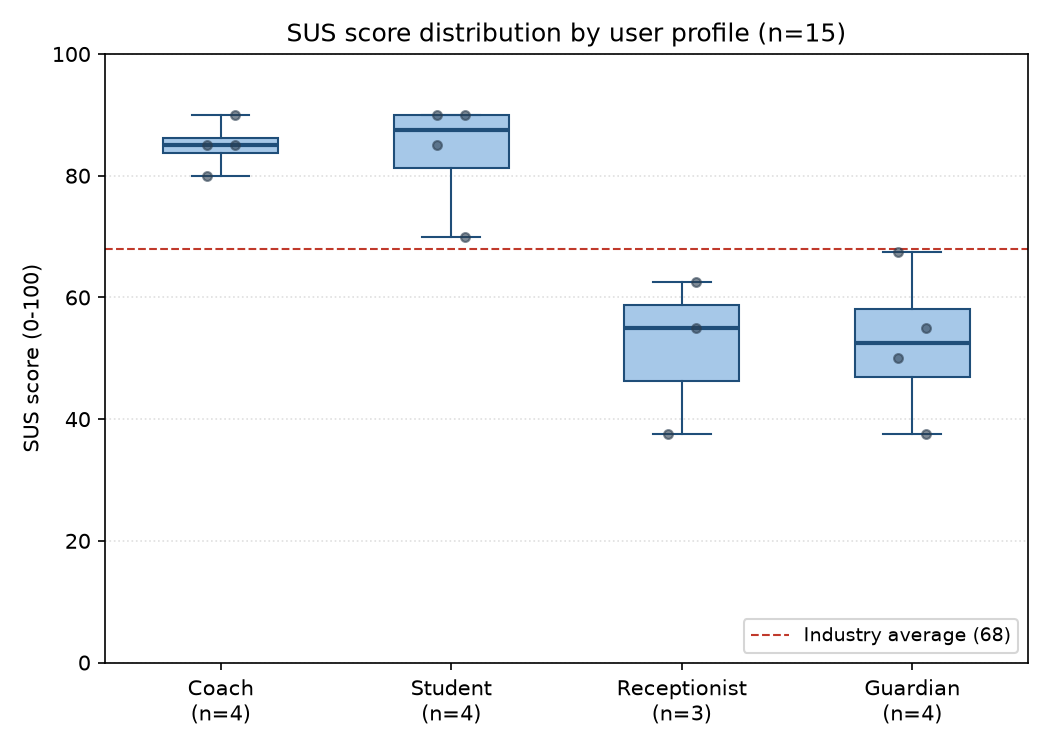
\includegraphics[width=0.75\textwidth]{../mediciones/sus/sus-boxplot.png}
\caption{Distribución de puntuaciones SUS por perfil (diagrama de caja), generado por \ruta{scripts/sus-boxplot.py} a partir de \ruta{docs/mediciones/sus/respuestas.csv}. La línea punteada marca la media de la industria (SUS~=~68).}
\label{fig:sus-boxplot}
\end{figure}

La Figura~\ref{fig:sus-boxplot} muestra de un vistazo lo que la Tabla~\ref{tab:sus-perfil}
solo da como promedios: los cuatro perfiles se parten en dos bloques con muy poca dispersión interna:
1,2 puntos de diferencia dentro del grupo alto, 0,8 dentro del bajo, y 33,3
entre ambos --- más de una vez y media la amplitud del intervalo de confianza.

La línea divisoria no es ser interno o externo a la escuela: el recepcionista
es personal interno y de uso diario, y puntúa igual de bajo que el
representante. Lo que separa a los grupos es \emph{qué hace cada rol con el
sistema}. Entrenador y estudiante sobre todo consultan --- ver sesiones,
marcar asistencia, revisar el equipo ---, y esos son los flujos que más
atención de diseño recibieron. Recepcionista y representante operan o esperan
información: el primero da de alta, edita y cobra; el segundo busca
visibilidad sobre su representado y hoy el sistema no le envía nada por
iniciativa propia (RF-22 sigue sin implementarse). Dicho de otro modo, quien
peor califica el sistema es quien más trabajo administrativo hace con él.

El patrón resistió dos ampliaciones sucesivas de la muestra: los cinco
participantes agregados --- dos estudiantes, dos representantes y un
entrenador --- cayeron cada uno en el bloque que su rol predecía, sin
excepción. Es una pista concreta de dónde enfocar el trabajo de usabilidad,
no solo un número que aprobó por poco.

Con 3 o 4 participantes por perfil estos promedios son indicativos y no
soportan una prueba de hipótesis entre grupos: el patrón se sostiene por su
magnitud y por su consistencia al ampliar la muestra, no por significancia
estadística. El análisis completo, con las amenazas a la validez, está en
\ruta{docs/mediciones/sus/INTERPRETACION.md}.

% ============================================================
\section{Reproducibilidad}

El sistema se levanta completo desde una clonación limpia con un solo
comando, siguiendo la misma motivación que documentan Cito y Gall para
usar contenedores como mecanismo de reproducibilidad en investigación
de ingeniería de software: encapsular las suposiciones y dependencias
que de otro modo quedan como conocimiento tácito del
equipo~\cite{citogall2016docker} (Listado~\ref{lst:arranque-reproducible}):

\begin{lstlisting}[language=bash,caption={Arranque reproducible},label={lst:arranque-reproducible}]
git clone https://github.com/gleiston-guerrero/SGED_APPWEB.git
cd SGED_APPWEB
cp .env.example .env
make up
make carga   # volumen sintetico (2401 estudiantes) para reproducir la sec. de rendimiento
\end{lstlisting}

El mismo \texttt{Makefile} expone, además del arranque, los objetivos
que reproducen cada bloque de evidencia de este informe
(Tabla~\ref{tab:makefile-objetivos}):

\begin{table}[htbp]
\centering
\caption{Objetivos del Makefile para reproducción end-to-end.}
\label{tab:makefile-objetivos}
\begin{tabular}{@{}ll@{}}
\toprule
\textbf{Objetivo} & \textbf{Acción} \\
\midrule
\texttt{make up} & Levanta el sistema completo \\
\texttt{make test} & JUnit 5 + cobertura JaCoCo \\
\texttt{make bench} & 5 corridas k6 por escenario (cálida y fría) + análisis inferencial con IC 95\,\% \\
\texttt{make carga} / \texttt{make limpiar-carga} & Sembrar / retirar el volumen sintético para reproducir el benchmark \\
\texttt{make audit} & Auditoría OWASP (6 controles) + SQL dinámico \\
\texttt{make clean} & Limpia contenedores, volúmenes y compilaciones \\
\bottomrule
\end{tabular}
\end{table}

Las imágenes de PostgreSQL y Redis están fijadas por digest SHA-256, no por
etiqueta móvil: dos construcciones del mismo \emph{commit} usan exactamente
los mismos binarios. La reproducibilidad se verificó clonando el repositorio
en un directorio independiente, no solo reiniciando el volumen local.

% ============================================================
\section{Amenazas a la validez}
\label{sec:amenazas}

Los resultados de la sección anterior cumplen los umbrales exigidos, pero
cumplirlos no equivale a ser generalizables. Esta sección declara las
limitaciones que acotan hasta dónde puede sostenerse cada conclusión,
siguiendo la clasificación habitual en ingeniería de software
empírica~\cite{iso25010}.

\subsection{Validez de constructo}

\emph{¿Mide cada indicador lo que se pretende medir?}

\begin{itemize}[leftmargin=*]
  \item \textbf{La cobertura de instrucciones no mide calidad de las
    pruebas.} Un 88,38\,\% indica qué proporción del código se ejecuta
    durante la suite, no que las aserciones sean pertinentes —el mismo
    desacople que documentan Imran~\emph{et al.} sobre pruebas de
    rendimiento en sistemas Java de código abierto: alcanzan una
    cobertura sistemáticamente menor que las pruebas funcionales pese a
    ser igual de válidas, porque miden algo distinto de lo que la
    cobertura agregada expresa~\cite{imran2025coverage}. El caso del
    registro de usuarios lo demuestra dentro de este mismo proyecto: el
    \emph{endpoint} estaba cubierto por dos pruebas que pasaban y aun así
    fallaba en toda petición real (sección~\ref{sec:defectos-runtime}).
  \item \textbf{La auditoría OWASP verifica controles, no ausencia de
    vulnerabilidades.} Comprueba seis controles concretos del Top 10 con
    peticiones dirigidas. No es una prueba de penetración ni un análisis
    estático: que los seis den correcto no permite afirmar que el sistema
    sea seguro, solo que esos seis comportamientos son los esperados.
  \item \textbf{El SUS mide usabilidad percibida, no desempeño.} No se
    registraron tiempos ni tasas de finalización por tarea, de modo que un
    participante pudo puntuar alto sin haber completado las tareas
    propuestas. Las columnas de completitud del CSV quedaron vacías y se
    declaran vacías en lugar de rellenarse.
\end{itemize}

\subsection{Validez interna}

\emph{¿Puede algo distinto de lo declarado explicar los resultados?}

\begin{itemize}[leftmargin=*]
  \item \textbf{Las mediciones de rendimiento se tomaron en la misma
    máquina que ejecuta el sistema}, sin latencia de red real. Los
    19,94\,ms de p95 en caché cálida (38,20\,ms en fría) son un límite
    inferior optimista: en un despliegue con red de por medio la cifra
    sería mayor, aunque el margen frente al umbral de 200\,ms es amplio.
  \item \textbf{Cinco corridas por escenario son pocas} para caracterizar
    una distribución. Se reporta el intervalo de confianza al 95\,\% para
    no presentar una única corrida como si fuera el valor verdadero, pero
    con $n=5$ ese intervalo es ancho.
  \item \textbf{La base de datos de las mediciones contiene datos
    sembrados, no un volumen de producción.} El rendimiento de las
    consultas paginadas sobre un catálogo pequeño no anticipa el
    comportamiento con miles de estudiantes.
\end{itemize}

\subsection{Validez externa}

\emph{¿Hasta dónde se generalizan los resultados?}

\begin{itemize}[leftmargin=*]
  \item \textbf{La muestra del SUS es de 15 participantes},
    recolectada por conveniencia. Cumple el mínimo exigido, pero el
    intervalo de confianza (58,87--79,79) todavía incluye valores por
    debajo del umbral de 68: 69,33 es la mejor estimación puntual
    disponible, no un aprobado consolidado.
  \item \textbf{Los subgrupos por perfil tienen 3 o 4 personas cada uno.}
    El patrón bimodal es nítido y tiene una explicación plausible ligada a
    qué flujos están implementados, pero con esos tamaños no puede
    descartarse que parte de la diferencia sea variación individual. Se
    presenta como hipótesis orientadora para la Entrega Final, no como
    conclusión establecida.
  \item \textbf{Los resultados describen este sistema en este entorno.} No
    se comparan contra un sistema de referencia ni contra una versión
    anterior medida en las mismas condiciones.
\end{itemize}

\subsection{Validez de conclusión}

El riesgo principal de este informe no es estadístico sino de
procedimiento, y ya se materializó tres veces: \textbf{un indicador puede
dar verde sobre un sistema que no hace lo que el indicador afirma}
(sección~\ref{sec:a01-falso-correcto}). Las tres ocurrencias se corrigieron
en su origen, pero la lección se declara aquí porque acota la confianza que
merece cualquier cifra de este documento: son válidas en tanto la medición
se ejecute contra el sistema real, desde estado limpio, y verificando las
dos direcciones del comportamiento esperado.

Queda además una divergencia sin resolver que afecta la reproducibilidad a
futuro: el esquema consolidado que crea la base de datos
(\ruta{db/schema.sql}) y las migraciones Flyway versionadas describen
estructuras distintas, porque las segundas no se actualizaron tras la
reestructuración y hoy no se ejecutan (\texttt{FLYWAY\_ENABLED=false}). El
sistema arranca de forma reproducible por la primera vía, que es la
verificada en este informe, pero la decisión sobre cuál de las dos fuentes
queda como autoritativa está pendiente y se declara abierta.

Finalmente, \textbf{el DOI de Zenodo ya está asignado}: el corte
\texttt{v1.0.0} de este repositorio está archivado con DOI
\href{https://doi.org/10.5281/zenodo.22739944}{10.5281/zenodo.22739944}
(concept DOI~\href{https://doi.org/10.5281/zenodo.21713239}{10.5281/zenodo.21713239},
que resuelve directamente a esta versión), publicado el 2026-09-14 como
nueva versión de la misma serie mediante la integración
GitHub\,\textrightarrow\,Zenodo sobre el \emph{release} de esa etiqueta
republicado tras el corte final defendido, lo que
satisface el archivo permanente exigido por el Bloque~E.2. Supera a la
versión anterior de la misma serie
(\href{https://doi.org/10.5281/zenodo.22714477}{10.5281/zenodo.22714477},
corte 2026-09-11). Un depósito anterior, publicado por error como
registro independiente en vez de nueva versión de esta serie
(corte \texttt{v1.0.1}), quedó retirado en Zenodo (HTTP~410) y por eso
ya no se cita. La
versión \texttt{v0.9.0-rc} del repositorio anterior es la primera de esta
misma serie y conserva su propio DOI de versión
(\href{https://doi.org/10.5281/zenodo.21713240}{10.5281/zenodo.21713240}).

% ============================================================
\section{Consideraciones éticas}
\label{sec:etica}

El sistema trata datos personales de niños, niñas y adolescentes: nombres,
cédula, fecha de nacimiento, asistencia con hora y lugar, y evaluaciones
individuales de desempeño. Esa combinación es sensible porque los titulares
son menores que no pueden consentir por sí mismos, porque la asistencia es
información de localización temporal, y porque las evaluaciones constituyen
perfilado de personas~\cite{lopdp2021,acm2018}. El riesgo no es solo
regulatorio: Carvalho y Gonçalves advierten sobre la presión creciente por
identificar talento a edades cada vez más tempranas en el deporte
formativo, y sobre el desajuste entre los indicadores que se miden y el
desarrollo real del deportista
joven~\cite{carvalho2023talento}. Un sistema que registra
puntajes periódicos de un menor no es un instrumento neutral: puede
consolidar una etiqueta temprana que condicione decisiones posteriores
sobre esa misma persona.

El principio de minimización se aplicó al diseño original —se descartaron
contextura y datos de alimentación—, pero conviene ser preciso sobre su
alcance real, porque la versión anterior de este informe afirmaba que
tampoco se recolectaban peso y altura y \textbf{esa afirmación ya no es
cierta}: la reestructuración incorporó ambas columnas a
\texttt{academico.estudiantes} y son exponibles por la API. El documento de
ética se corrigió (hallazgo H-06) en lugar de mantener la declaración
cómoda, y este informe se corrige aquí por la misma razón: una declaración
de minimización que no coincide con el esquema no protege a nadie.

\ruta{docs/etica/ETHICS.md} documenta nueve hallazgos, en lugar de afirmar
que todo está resuelto: la cédula se almacena sin validación ni cifrado
(H-01); las observaciones del entrenador son texto libre sin control sobre
un menor (H-02); la baja lógica preserva el historial pero no es un borrado,
por lo que hacía falta un mecanismo de supresión efectivo —resuelto el
2026-09-08 con el procedimiento de anonimización de RF-50— (H-03); el consentimiento del
representante no está modelado, lo que bloquea el módulo de notificaciones
(H-04); el certificado TLS era autofirmado —resuelto el 2026-09-09 con el
despliegue en Render, que sirve HTTPS con certificado de una autoridad
reconocida— (H-05); peso y altura se agregaron sin base legal
documentada —resuelto el 2026-09-09: finalidad y base legal declaradas,
lectura restringida por rol y alcance de consentimiento propio— (H-06); y la
plantilla de consentimiento cubría a los evaluadores del SUS, no a los
representantes de los menores —resuelto el 2026-09-09 con
\ruta{docs/etica/consentimiento/representante.md}— (H-07).

El octavo, \textbf{H-08}, se registra ya corregido, y se deja escrito
justamente porque corregirlo en silencio habría sido lo fácil: los datos
identificativos de los estudiantes estuvieron accesibles a cualquier cuenta
autenticada del sistema, incluida la búsqueda por número de cédula
(sección~\ref{sec:a01-falso-correcto}). Un documento de ética que solo
enumera riesgos hipotéticos y omite la exposición concreta que sí ocurrió
sería un documento de imagen, no de rendición de cuentas.

\subsection{Generación de retroalimentación con un modelo de lenguaje externo}
\label{sec:ia-feedback}

El sistema incorpora un servicio opcional
(\ruta{backend/.../common/ia/GeminiFeedbackService.java}) que redacta
comentarios de retroalimentación deportiva invocando un modelo de lenguaje
de un tercero. Enviar información sobre menores de edad a un proveedor
externo es, por sí mismo, una superficie de divulgación nueva, así que las
decisiones de diseño se documentan aquí y no solo en el código:

\begin{itemize}[leftmargin=*]
  \item \textbf{Seudonimización estructural, no por convención.} Lo único
    que se serializa hacia el proveedor es el \emph{record}
    \texttt{PerfilJugadorAnonimo}, que no tiene campos de nombre, cédula,
    correo ni fecha de nacimiento. No es que el código «evite» enviarlos:
    no existen en el tipo que viaja, de modo que no hay forma de filtrarlos
    aunque una modificación futura lo intentara por descuido.
  \item \textbf{La clave viaja en cabecera, no como parámetro de consulta.}
    Ambas formas están documentadas por el proveedor, pero un parámetro de
    consulta queda registrado en \emph{logs} de acceso, historiales de
    \emph{proxy} y cabeceras \texttt{Referer}.
  \item \textbf{Desactivado por defecto y degradación silenciosa.} Sin
    clave configurada el servicio reporta no disponible y el resto de la
    evaluación funciona igual; un fallo del proveedor nunca puede hacer
    perder al entrenador lo que ya calificó a mano.
  \item \textbf{Instrucción de sistema que prohíbe inventar.} El
    \emph{prompt} de sistema acota el registro, prohíbe explícitamente
    afirmar hechos que no estén en los datos numéricos recibidos, exige
    tono apropiado para un menor y veta diagnósticos médicos o
    recomendaciones de aumentar carga física a un jugador lesionado.
  \item \textbf{Los registros no incluyen el \emph{prompt}.} Ante un fallo
    se registra el tipo de excepción, nunca el contenido enviado.
\end{itemize}

Estas mitigaciones acotan el riesgo de divulgación, no la calidad del texto
generado, que es un problema distinto y abierto: Dai~\emph{et al.} muestran
que la retroalimentación producida por modelos de lenguaje puede ser fluida
y coherente y aun así variar en su pertinencia según el
criterio evaluado~\cite{dai2024feedback}. Por eso el comentario generado se
presenta como apoyo a la redacción del entrenador y no como sustituto de su
juicio, y su evaluación empírica queda declarada como trabajo pendiente:
\textbf{esta entrega no aporta evidencia sobre la calidad de los textos
generados}, solo sobre las garantías de privacidad de su integración.

Todos los datos del repositorio son ficticios. No se utilizaron datos reales
de menores en ninguna etapa del desarrollo ni de las mediciones.

% ============================================================
\section{Declaración de contribuciones (CRediT)}
\label{sec:credit}

Los roles siguientes no son autodeclarados: se derivan del historial de
\texttt{git} del repositorio y cada uno puede verificarse con
\texttt{git log --author}. Las cifras provienen de \texttt{git log
--numstat} sobre la rama \texttt{main} y separan lo \emph{escrito} de lo
\emph{generado} (reportes de JaCoCo y Lighthouse, salidas crudas de k6,
\texttt{package-lock.json}, PDF), porque contar un reporte HTML de
cobertura como líneas de autoría inflaría la medida sin reflejar trabajo
(Tabla~\ref{tab:credit-cifras}).

\begin{table}[htbp]
\centering
\caption{Evidencia cuantitativa de autoría por integrante (\texttt{git log} sobre \texttt{main}, medido el 2026-09-12, commit \texttt{6fd0581}). La misma medición está en \ruta{CONTRIBUTORS.md}, y cambia con cada commit nuevo por diseño: la cifra que cuenta es la que resulte de correr el comando de esa tabla sobre el commit que finalmente se defienda. Arcalle Grefa suma los commits de sus dos correos vinculados a la misma cuenta de GitHub (\texttt{darcalleg@uteq.edu.ec} y \texttt{darwinarcalle@gmail.com}).}
\label{tab:credit-cifras}
\begin{tabular}{@{}lrrr@{}}
\toprule
\textbf{Integrante} & \textbf{\emph{Commits}} & \textbf{Líneas escritas} & \textbf{Archivos} \\
\midrule
Pallo Pinto Alejandro Daniel & 233 & 82\,050 & 792 \\
Arcalle Grefa Darwin Orlando & 136 & 60\,993 & 776 \\
Velez Lopez Ricardo Elias & 55 & 11\,912 & 153 \\
\midrule
\textbf{Total en \texttt{main}} & \textbf{424} & \textbf{154\,955} & \textbf{1\,721} \\
\bottomrule
\end{tabular}
\end{table}

\subsection{Roles por integrante}

\textbf{Pallo Pinto Alejandro Daniel} — \emph{Conceptualización},
\emph{Curación de datos}, \emph{Análisis formal}, \emph{Investigación},
\emph{Metodología}, \emph{Recursos}, \emph{Software}, \emph{Validación},
\emph{Visualización}, \emph{Redacción (borrador original)}, \emph{Redacción
(revisión y edición)}.

Responsable de la totalidad del eje de verificación que define esta
entrega. En seguridad: migración del JWT de \texttt{localStorage} a cookie
\texttt{HttpOnly}+\texttt{Secure}+\texttt{SameSite}, terminación TLS,
CSP explícito, registro de auditoría A09, y la corrección del control de
acceso ausente en los cinco recursos nuevos (H-08,
sección~\ref{sec:a01-falso-correcto}). En datos: conversión de las
funciones PL/pgSQL a procedimientos reales invocables con
\texttt{@Procedure} (sección~\ref{sec:acceso-datos}) y fijación de
imágenes por digest. En validación: las 57 pruebas que cerraron la
primera regresión de cobertura (la suite siguió creciendo después, hasta
las 576 actuales —sección~\ref{sec:cobertura}—), la corrección del defecto
por el que JaCoCo nunca había medido cobertura real, y las tres campañas
de medición empírica (k6, OWASP, Lighthouse) junto con sus \emph{scripts}
de análisis. En usabilidad: instrumento SUS, \emph{script} de cálculo
validado contra los casos de referencia de la literatura, y transcripción
de las diez encuestas. En redacción: este informe y el corpus documental
(SRS, casos de uso, historias, matriz de trazabilidad, ADR, ética,
diccionario de datos, gobernanza del repositorio).

\textbf{Arcalle Grefa Darwin Orlando} — \emph{Conceptualización},
\emph{Curación de datos}, \emph{Análisis formal}, \emph{Investigación},
\emph{Metodología}, \emph{Administración del proyecto}, \emph{Recursos},
\emph{Software}, \emph{Supervisión}, \emph{Validación},
\emph{Visualización}, \emph{Redacción (borrador original)}, \emph{Redacción
(revisión y edición)}.

Estructura inicial del repositorio y del modelo de datos
(\texttt{DataBase/}), trabajo sobre el \emph{frontend} Angular
(componentes, \emph{Dockerfile} y configuración de formato), y
administración del repositorio remoto, del que es propietario.
Participación en la reestructuración en dominios
\texttt{academico}/\texttt{deportivo}/\texttt{seguridad} descrita en la
sección~\ref{sec:reestructuracion}. Relevamiento de requisitos con la
escuela ProFútbol y recolección de evidencia empírica (\emph{Investigación}),
y coordinación del equipo, calendario y entregas a lo largo de las cuatro
fases (\emph{Administración del proyecto} y \emph{Supervisión}).

\textbf{Velez Lopez Ricardo Elias} — \emph{Conceptualización},
\emph{Curación de datos}, \emph{Análisis formal}, \emph{Metodología},
\emph{Recursos}, \emph{Software}, \emph{Validación}, \emph{Visualización},
\emph{Redacción (borrador original)}, \emph{Redacción (revisión y edición)}.

Arranque del \emph{frontend} Angular y del módulo de autenticación, CRUD
inicial de \texttt{Estudiante}, y aportes a \ruta{docs/requisitos/} y
\ruta{docs/observaciones/}. Autor principal de la reestructuración en tres
dominios y de los cinco recursos CRUD nuevos, que es el cambio estructural
sobre el que se apoya esta entrega. Definición del proceso de
investigación (DSR) y del protocolo de medición (\emph{Metodología}),
configuración del entorno de despliegue en Render y de los contenedores
Docker (\emph{Recursos}), y revisión de la documentación y su consistencia
con el código (\emph{Redacción: revisión y edición}).

\subsection{Cobertura de los catorce roles CRediT}

La taxonomía CRediT define catorce roles. Trece quedan cubiertos por el
equipo; \emph{Adquisición de fondos} no aplica a un Proyecto Fin de Curso
sin financiamiento externo (Tabla~\ref{tab:credit-cobertura}). La misma
tabla está en \ruta{CONTRIBUTORS.md}. El número junto a cada integrante
ya no es su total de \emph{commits} repetido en cada fila (así estaba
hasta el 2026-09-13, y no distinguía nada específico de cada rol): es el
número de \emph{commits} de esa persona que tocaron al menos un archivo
de las rutas asociadas a ese rol, con el mapeo rol\,\textrightarrow\,rutas
declarado y reproducible en \texttt{scripts/credit-counts.py}. CRediT
clasifica tipos de contribución intelectual, no una partición exclusiva
de archivos —un mismo \emph{commit} puede sostener varios roles a la
vez—. Cuatro roles (\emph{Investigación}, \emph{Metodología},
\emph{Administración del proyecto} y \emph{Supervisión}) incluyen trabajo
real que no deja huella en el árbol de archivos —reuniones con la
escuela ProFútbol, coordinación del equipo, decisiones de calendario— y
se declaran así en vez de asignarles un número inventado.

\begin{table}[htbp]
\centering
\scriptsize
\caption{Cobertura de los catorce roles de la taxonomía CRediT (conteos de \texttt{scripts/credit-counts.py f2c0f11}).}
\label{tab:credit-cobertura}
\begin{tabular}{@{}p{3.2cm}p{3.4cm}p{7.2cm}@{}}
\toprule
\textbf{Rol CRediT} & \textbf{Integrante(s)} & \textbf{Cobertura} \\
\midrule
Conceptualización & Darwin (45), Alejandro (26), Ricardo (6) & Diseño de los cuatro dominios (académico, deportivo, inventario, seguridad) y de la estrategia híbrida de acceso a datos. \\
Curación de datos & Alejandro (49), Darwin (27), Ricardo (6) & Diseño del esquema, procedimientos almacenados y limpieza de los datos crudos de medición. \\
Análisis formal & Alejandro (11), Darwin (5), Ricardo (4) & Análisis estadístico de los datos de rendimiento y usabilidad (intervalos de confianza, distribución \emph{t}). \\
Adquisición de fondos & --- & No aplica (proyecto académico sin financiación externa). \\
Investigación & Alejandro (3), Darwin (2)* & Relevamiento de requisitos con la escuela ProFútbol y recolección de evidencia empírica. \\
Metodología & Alejandro (4), Ricardo (2), Darwin (2)* & Proceso de investigación (DSR) y protocolo de medición. \\
Administración del proyecto & Darwin* & Administración del proyecto, calendario y gestión de entregas. \\
Recursos & Alejandro (12), Darwin (14), Ricardo (7) & Configuración del entorno de despliegue (Render), contenedores Docker y base de datos. \\
Software & Alejandro (128), Darwin (54), Ricardo (12) & Implementación de backend (Spring~Boot), \emph{frontend} (Angular) y procedimientos almacenados. \\
Supervisión & Darwin* & Coordinación del equipo y seguimiento del repositorio. \\
Validación & Alejandro (72), Darwin (43), Ricardo (11) & Cobertura (JaCoCo), pruebas de carga (k6), estudio de usabilidad (SUS) y auditoría de seguridad. \\
Visualización & Darwin (7), Alejandro (4), Ricardo (3) & Diagramas C4 y de arquitectura del sistema. \\
Redacción (borrador original) & Darwin (63), Alejandro (60), Ricardo (15) & Redacción del informe, del SRS y de la documentación técnica. \\
Redacción (revisión y edición) & Darwin (108), Alejandro (87), Ricardo (26) & Revisión y corrección de la documentación y su consistencia con el código. \\
\bottomrule
\end{tabular}
\end{table}

\noindent\small(*) Investigación, Metodología, Administración del proyecto
y Supervisión incluyen trabajo real que no deja huella en el árbol de
archivos (reuniones con la escuela ProFútbol, coordinación del equipo,
decisiones de calendario); el número que sí aparece es solo la parte que
además dejó un \emph{commit} sobre un archivo relacionado, no el total del
trabajo.\normalsize

\subsection{Dos advertencias sobre la medida}

\textbf{El volumen no es la contribución.} Las líneas escritas miden
actividad, no valor: un cambio de dos líneas que corrige un fallo de
control de acceso pesa más que dos mil líneas de documentación. La tabla
se incluye porque el criterio de evaluación exige autoría verificable, no
para establecer una jerarquía entre integrantes.

\textbf{La identidad de \texttt{git} quedó unificada en correos
institucionales.} Al preparar el repositorio para la Entrega Final se
reorganizó el historial para que todos los \emph{commits} de \texttt{main}
quedaran atribuidos a los tres correos \texttt{@uteq.edu.ec} del equipo
(\texttt{dpallop}, \texttt{rvelezl3}, \texttt{darcalleg}). El estado
anterior mezclaba correos personales (\texttt{outlook.es},
\texttt{gmail.com}), un tipeo (\texttt{uteq.edue.ec}) y dos \emph{commits}
del 2026-06-29 que —por la sesión configurada en un equipo de la
universidad— figuraban bajo la cuenta \texttt{DannaN24}, siendo trabajo de
\textbf{Pallo Pinto Alejandro Daniel} y ya sumados a su fila en la tabla
anterior. Ninguno de esos correos aparece ya en \texttt{git log}: solo la
atribución de autoría cambió, no el contenido de ningún archivo. La
comprobación se repite listando los autores de \texttt{main} con
\texttt{git log}; el detalle está en \ruta{CONTRIBUTORS.md}.

% ============================================================
\section{Trazabilidad y honestidad académica}

La matriz \ruta{docs/trazabilidad/matriz.csv} enlaza cada requisito con su
historia de usuario, su caso de uso, su \emph{endpoint}, el archivo que lo
implementa, la prueba JUnit que lo cubre y la evidencia empírica
correspondiente.

El historial de \texttt{git} evidencia la autoría de cada integrante. Al
preparar la Entrega Final se reorganizó ese historial para unificar la
identidad de cada autor en su correo institucional \texttt{@uteq.edu.ec}
—sin alterar el contenido de ningún archivo—, y \ruta{CONTRIBUTORS.md}
documenta el estado anterior y cómo verificar el resultado. El mismo
archivo declara explícitamente el uso de herramientas de asistencia por
inteligencia artificial, siguiendo la guía de transparencia del SWEBOK
v4.0~\cite{swebok2024}.

% ============================================================
\section{Discusión}
\label{sec:discusion}

\textit{Nota de versión: esta sección responde a las preguntas de
investigación (sección~\ref{sec:rqs}) sobre la evidencia remedida para la
Entrega Final y archivada en \ruta{docs/mediciones/}, no sobre las
corridas parciales que sirvieron a la Tercera Entrega. La distinción
importa porque aquellas antecedían al módulo de inventario y a parte del
dominio deportivo, y reportarlas sin remedir habría sido exactamente el
error que la sección~\ref{sec:defectos-runtime} documenta: un indicador
verde que no refleja el sistema real.}

\paragraph{RQ1 — Rendimiento.} Sí, con margen amplio. Las cinco corridas
independientes por escenario archivadas en \ruta{docs/mediciones/perf/}
(50 usuarios virtuales, 30\,s por corrida) dan, en caché cálida, una media
de 11{,}28\,ms (DT~2{,}93; IC~95\,\%~$\pm$~4{,}66) y un p95 de
19{,}94\,ms (IC~95\,\%~$\pm$~13{,}51) contra el \emph{endpoint} de
listado protegido. El umbral de la norma es 200\,ms con caché caliente:
el sistema queda un orden de magnitud por debajo, y la diferencia frente a
la caché fría (media 17{,}74\,ms, p95 38{,}20\,ms) es estadísticamente
significativa (Mann-Whitney bilateral, $p < 10^{-60}$ en cada corrida;
$p \approx 10^{-2483}$ en el pool; sección~\ref{sec:rendimiento},
Tabla~\ref{tab:inferencial}). El contraste es relevante, no decorativo:
la caché de Redis reduce el tiempo de respuesta del listado en
$\approx$6{,}5\,ms de media y $\approx$18\,ms en p95, un ahorro del
orden del 35--45\,\% frente al escenario frío.

\paragraph{RQ2 — Seguridad.} Los seis controles OWASP (A01, A02, A03, A05,
A07, A09) están verificados con evidencia reproducible en
\ruta{docs/mediciones/sec/} (sección~\ref{sec:a01-falso-correcto}), y una
revisión directa del código fuente y de \ruta{db/procs/} no encontró
ningún uso de \texttt{createNativeQuery} con concatenación, \texttt{@Query}
construida con \texttt{+}, ni \texttt{EXECUTE}/\texttt{sp\_executesql}
dentro de los procedimientos almacenados — la estrategia híbrida no
introdujo la superficie de ataque que introduciría SQL dinámico mal
construido. A esa revisión manual se suma la evidencia automática que exige la
Entrega Final, reproducible por un tercero sin depender de ella: el
escaneo con OWASP~ZAP en modo \emph{baseline}
(\ruta{docs/mediciones/sec/zap/}, informe en HTML, JSON y XML junto a la
configuración que lo genera) cierra con \textbf{cero hallazgos, de
cualquier severidad}, tras apagar en el ambiente público la interfaz de
Swagger UI que originalmente exponía una dependencia de terceros
desactualizada; una segunda corrida con sesión autenticada y
\emph{active scan} (sección~\ref{sec:zap-spotbugs}) confirma cero
hallazgos de inyección también bajo ataque activo. El análisis
estático (\ruta{docs/mediciones/sec/static-analysis/}) no reporta
ocurrencias de la regla
\texttt{SQL\_NONCONSTANT\_STRING\_PASSED\_TO\_EXECUTE}, que es la
comprobación automática equivalente a la inspección de código descrita
arriba.

\paragraph{RQ3 — Usabilidad.} La respuesta es clara y es, a la vez, el
hallazgo menos cómodo de todo el documento (sección~\ref{sec:sus}): la
usabilidad \textbf{no} es homogénea entre roles. El sistema obtiene grado
A en entrenadores y estudiantes y grado F en recepcionistas y
representantes, con una media agregada (68{,}25) que esconde ese patrón
bimodal en vez de exponerlo. La implicación práctica es directa: el
esfuerzo de mejora de interfaz debería priorizar el flujo administrativo y
el futuro módulo de representantes, no el promedio general del sistema.
Con los quince participantes que exige la Entrega Final la media es
69{,}33 (IC~95\,\%~58{,}87--79{,}79), y la ampliación de diez a quince
resultó informativa por una razón que conviene explicitar: la media se
movió apenas 1{,}08 puntos mientras el intervalo de confianza se estrechó
en torno a un tercio. Es decir, los cinco cuestionarios adicionales precisaron la
estimación en lugar de desplazarla, lo que refuerza el patrón bimodal en
vez de diluirlo. Aun así, con tres o cuatro participantes por rol la
desagregación sigue siendo indicativa y no una estimación poblacional.

\paragraph{RQ4 — Cobertura y trazabilidad bajo crecimiento.} Esta pregunta
nace directamente de un patrón que ya se repitió una vez en la Segunda
Entrega (sección~\ref{sec:reestructuracion}): la cobertura cayó muy por
debajo del umbral cuando se agregaron cinco recursos nuevos sin pruebas
propias, y se corrigió por encima de él de nuevo. La pregunta para la
Entrega Final es si ese patrón
se repite con el módulo de inventario y el resto del dominio deportivo,
agregados después de esa medición. El reporte remedido para esta entrega
(\ruta{docs/mediciones/jacoco/jacoco.xml}) responde que el patrón
\textbf{no} se repitió: 88{,}38\,\% de líneas (3\,013 de 3\,409) y
74{,}20\,\% de ramas (791 de 1\,066) sobre el \texttt{main} que incluye ya
el módulo de inventario y el dominio deportivo completo (la cifra coincide
con la de la sección~\ref{sec:cobertura} y es la única vigente en el
documento). La comparación con el episodio de la Segunda Entrega es la que
da sentido a la pregunta: allí la cobertura cayó por debajo del umbral al
agregar cinco recursos sin pruebas propias y hubo que corregirla de
nuevo; aquí el crecimiento se acompañó de pruebas desde el principio y la
cifra subió en vez de caer.

La advertencia que motivó RQ4 sigue siendo pertinente como práctica:
el patrón puede volver a ocurrir si no se vuelve a medir explícitamente
en cada crecimiento futuro del dominio, de modo que la cobertura quede
vinculada a una corrida reproducible (\texttt{./mvnw verify}) y no a una
cifra declarada.

% ============================================================
\section{Trabajo futuro}
\label{sec:trabajo-futuro}

Cinco líneas de trabajo quedan fuera del alcance de esta entrega, cada una
con una razón concreta documentada en otra parte del proyecto — no son una
lista genérica de ideas, son los pendientes que \ruta{docs/etica/ETHICS.md}
y \ruta{VERSIONING.md} ya declaran abiertos.

\begin{enumerate}[leftmargin=*]
  \item \textbf{Envío proactivo de notificaciones al representante
    (RF-22).} La lectura de informes por un representante con vínculo
    activo ya funciona; el envío proactivo (push/email/SMS) queda fuera a
    propósito hasta no tener un mecanismo de consentimiento explícito y
    fechado, distinto del consentimiento general de matrícula (hallazgo
    H-04, resuelto parcialmente el 2026-08-03).
  \item \textbf{Mecanismo de supresión de datos (resuelto el 2026-09-08).}
    El sistema aplica baja lógica, no borrado físico, por integridad
    referencial del historial deportivo. Para atender el derecho de
    supresión del representante se añadió el procedimiento almacenado
    versionado \texttt{academico.sp\_anonimizar\_estudiante} (migración
    \texttt{V27}), invocado por \texttt{POST /api/estudiantes/\{id\}/anonimizar}
    — solo \texttt{ADMINISTRADOR}, auditado —: sustituye los datos
    identificativos por valores neutros y borra el texto libre sobre el
    menor, conservando claves foráneas y estadísticas agregadas
    (hallazgo H-03, requisito RF-50).
  \item \textbf{Base legal documentada para peso y altura (resuelto el
    2026-09-09; RF-11c declarado el 2026-09-12).} Estos dos campos son
    datos de salud de un menor; se documentó su finalidad (seguimiento
    físico-deportivo, sin ranking ni decisiones automatizadas) y su base
    legal (consentimiento del representante con alcance propio
    \texttt{DATOS\_FISICO\_DEPORTIVOS}, registrado por RF-39), y la
    lectura del \emph{endpoint} de escritura ya existente se restringió a
    \texttt{ADMINISTRADOR}/\texttt{ENTRENADOR} (hallazgo H-06, requisito
    RF-11b, sección~\ref{sec:etica}). Queda una línea de trabajo menor,
    ya declarada como requisito propio y no como comentario suelto: RF-11c
    exigirá ese consentimiento como precondición del alta, en vez de
    admitirlo de forma incondicional como hoy.
  \item \textbf{Validación y protección de la cédula.} Hoy es un
    \texttt{VARCHAR(10)} sin validación de dígito verificador, sin
    restricción de unicidad y sin cifrado en reposo (hallazgo H-01) — más
    permisivo de lo deseable para un identificador nacional de un menor en
    un despliegue con datos reales.
  \item \textbf{Cerrar la brecha de usabilidad por rol.} La sección
    anterior (RQ3) encontró grado F en recepcionistas y representantes.
    Rediseñar específicamente esos dos flujos —no el sistema en general— y
    volver a medir SUS por subgrupo con $N \geq 15$ es la línea de trabajo
    con el respaldo empírico más directo de todo este documento.
\end{enumerate}

% ============================================================
\section{Conclusiones}

Retomando lo declarado en el resumen (sección~\ref{sec:resumen-es}) y en
el \emph{abstract} (sección~\ref{sec:resumen-en}), los hallazgos de este
trabajo se resumen así:

\begin{enumerate}[leftmargin=*]
  \item El sistema cumple con holgura los umbrales cuantitativos exigidos:
    p95 de 19,94\,ms en caché cálida (38,20\,ms en fría, un contraste
    significativo con $p \approx 10^{-2483}$) frente a un límite de
    200\,ms, 6 de 6 controles OWASP
    verificados con evidencia reproducible, accesibilidad Lighthouse de
    100/100, y \textbf{88,38\,\%} de cobertura de líneas y
    \textbf{74,20\,\%} de \emph{branches} frente al mínimo de 70\,\%
    (sección~\ref{sec:cobertura}) — cifra que cayó dos veces por debajo
    del umbral a medida que el sistema creció (tras la reestructuración
    de paquetes, y tras agregar el módulo de alertas y un segundo
    proveedor de IA) y se recuperó las dos veces con
    pruebas dirigidas al déficit real, no reportando directamente un
    número cómodo. El margen sobre el umbral, de apenas 0,06 puntos en
    el cierre provisional del 2026-09-02, se llevó a 1,24 puntos
    cubriendo los cuatro controladores en cero y las devoluciones de
    ciclo de vida de las entidades.

  \item \textbf{Una medición que no se ejecuta contra el sistema real no es
    evidencia.} Es la lección transversal de esta entrega, y aparece tres
    veces con la misma forma. La cobertura de JaCoCo se midió sobre un
    \texttt{target/} con clases previas a la reestructuración e incluía
    paquetes que ya no existen. La auditoría OWASP A01 devolvía
    \texttt{401} en todo y eso se parecía a un resultado correcto, cuando en
    realidad su propio control A07 la había dejado bloqueada. Y el registro
    de usuarios (RF-01) estaba roto contra la base de datos desde la
    reestructuración mientras sus dos pruebas unitarias pasaban, porque
    mockean el repositorio y la restricción la aplica PostgreSQL. En los
    tres casos el indicador era verde y el sistema no hacía lo que el
    indicador decía. Las tres mediciones se corrigieron en su origen —
    \texttt{make test} pasa a \texttt{clean test}, la auditoría limpia su
    propio contador y comprueba recurso por recurso— para que el defecto no
    pueda repetirse sin ser visible.

  \item El aporte más sustantivo de esta entrega no fue añadir
    funcionalidad, sino \emph{verificar} lo que ya existía, dos veces: una
    vez contra el código de la entrega original, y una segunda vez después
    de que otros dos integrantes reestructuraran el backend en paralelo.
    Ambas rondas revelaron defectos que ninguna revisión superficial había
    detectado — desde que JaCoCo no medía cobertura en absoluto, hasta que
    un ADR de arquitectura describía un mecanismo de autenticación
    (JWT en \texttt{localStorage}) distinto del que el código realmente usa
    (cookie \texttt{HttpOnly}), pasando por el control de acceso ausente en
    los cinco recursos nuevos (H-08). Todos los defectos encontrados se
    corrigieron y quedan documentados en las
    secciones~\ref{sec:reestructuracion} y~\ref{sec:defectos-runtime} en vez
    de ocultarse.

  \item La distinción entre lo implementado y lo modelado se mantiene
    explícita en todo el documento. En el caso de \texttt{Representante} y
    \texttt{Equipo} se llevó un paso más allá: en vez de dejar catorce
    clases vacías —una de ellas de cero bytes, el mismo defecto que motivó
    tres observaciones del docente en la Entrega 1B— se eliminaron del
    código y ambos módulos quedan declarados como pendientes solo en la
    documentación (sección~\ref{sec:reestructuracion}). Un archivo vacío no
    cuenta como funcionalidad entregada, y tampoco debería quedarse en el
    repositorio aparentando que sí.

  \item La encuesta SUS (sección~\ref{sec:sus}) ya no es un frente abierto,
    pero su resultado abre uno nuevo: el sistema es excelente para
    entrenadores y estudiantes (grado A) e inaceptable para recepcionistas
    y padres de familia (grado F). Mejorar la usabilidad del flujo
    administrativo y del futuro módulo de representantes es, con evidencia
    real detrás, más urgente que subir la media agregada. La exposición
    REST del dominio deportivo restante (horarios, sesiones, asistencias,
    evaluaciones) sigue siendo el objetivo natural de la Entrega Final.
\end{enumerate}

% ============================================================
\section{Declaraciones obligatorias}
\label{sec:declaraciones}

Sección propia y consolidada, exigida por el Bloque~B.15 de la Guía de
la Entrega Final. Las declaraciones de ética y de contribuciones
(CRediT) ya se desarrollaron con su propio detalle en las secciones
correspondientes de este documento; aquí se referencian en vez de
duplicarse, junto con las declaraciones que todavía no tenían una
sección propia.

\textbf{Disponibilidad de código.} Repositorio público en
\url{https://github.com/gleiston-guerrero/SGED_APPWEB}, etiqueta \texttt{v1.1.0}
(corte defendido del examen suspenso). El DOI del software sigue
anclado al corte anterior, \texttt{v1.0.0} (republicarlo sobre
\texttt{v1.1.0} queda pendiente; ver \texttt{VERSIONING.md}). DOI del software en
Zenodo: \href{https://doi.org/10.5281/zenodo.22739944}{10.5281/zenodo.22739944}
(concept DOI
\href{https://doi.org/10.5281/zenodo.21713239}{10.5281/zenodo.21713239}).

\textbf{Disponibilidad de datos.} Los datos crudos de todas las
mediciones (rendimiento, seguridad, cobertura, calidad web, usabilidad)
están versionados en \ruta{docs/mediciones/} bajo la misma licencia del
repositorio. El depósito separado del \emph{dataset} de mediciones está
publicado en Zenodo con DOI propio (\href{https://doi.org/10.5281/zenodo.22422305}{10.5281/zenodo.22422305})
y licencia Creative Commons Attribution~4.0.

\textbf{Disponibilidad de materiales.} Colección Postman
(\ruta{docs/postman/coleccion.json}, 32 peticiones, que cubre el catálogo
de la API de la sección~\ref{sec:catalogo-api}), \emph{scripts} de
carga k6 (\ruta{k6/}), configuración Lighthouse
(\ruta{lighthouserc.js}), instrumento y protocolo SUS
(\ruta{docs/mediciones/sus/INSTRUMENTO-SUS.md}), plantilla de
consentimiento (\ruta{docs/etica/consentimiento/}). \textbf{Pendiente:}
los análisis de rendimiento y de SUS son \emph{scripts} de Python
(\ruta{scripts/perf-analysis.py}, \ruta{scripts/sus-analysis.py}) y no
cuadernos ejecutables con salidas archivadas (Jupyter o RMarkdown) como
exige literalmente el Bloque~D.1; convertirlos o documentar la
equivalencia es una tarea abierta antes del cierre.

\textbf{Declaración ética.} El sistema trata datos personales de
menores de edad. Los participantes de la encuesta SUS firmaron
consentimiento informado, sus respuestas se anonimizaron con códigos
P01–P10, y nueve hallazgos éticos (H-01 a H-09, uno ya corregido) están
declarados sin omisiones en \ruta{docs/etica/ETHICS.md} y en la sección
de Consideraciones éticas de este documento.

\textbf{Contribuciones de autores (CRediT).} De los catorce roles de la
taxonomía CRediT, trece quedan cubiertos por el equipo; el único que no
aplica es \emph{Adquisición de fondos}, al ser un Proyecto Fin de Curso
sin financiamiento externo. El reparto —\emph{Conceptualización}
(Ricardo, Darwin), \emph{Curación de datos}, \emph{Análisis formal},
\emph{Visualización} y \emph{Redacción (borrador original)} (Alejandro),
\emph{Investigación}, \emph{Administración del proyecto} y
\emph{Supervisión} (Darwin), \emph{Metodología}, \emph{Recursos} y
\emph{Redacción (revisión y edición)} (Ricardo), \emph{Validación}
(Alejandro, Ricardo) y \emph{Software} (los tres)— se deriva de la
evidencia del historial de \texttt{git}, no es autodeclarado. El detalle
por integrante y la tabla de cobertura rol por rol están en la
sección~\ref{sec:credit} y en \ruta{CONTRIBUTORS.md}.

\textbf{Conflictos de interés.} El equipo declara la ausencia de
conflictos de interés: ningún integrante tiene relación contractual,
financiera o personal con la escuela ProFútbol ni con ningún proveedor
mencionado en este documento (Render, Supabase, GitHub, Google/Gemini y
Zenodo) más allá del uso de sus capas gratuitas para este proyecto
académico.

\textbf{Financiamiento.} Este trabajo no recibió financiamiento externo.
Es un Proyecto Fin de Curso de la asignatura Aplicaciones Web,
desarrollado como requisito académico de la Universidad Técnica Estatal
de Quevedo, sin patrocinio de terceros.

\textbf{Uso de asistentes de inteligencia artificial.} Distinto del uso
de un modelo de lenguaje como funcionalidad del propio sistema
(sección~\ref{sec:ia-feedback}), este apartado declara el uso de IA
generativa en el \emph{proceso} de construir el proyecto. Siguiendo la
guía de transparencia del SWEBOK v4.0~\cite{swebok2024}, el equipo
declara el uso de un asistente de IA generativa (Claude, de Anthropic)
como herramienta de apoyo en revisión y corrección de código de
seguridad, generación de \emph{scripts} de auditoría y análisis de
resultados, y redacción de documentación (incluidas partes de este
informe). El diseño de la arquitectura, las decisiones de seguridad y la
verificación de que el sistema funciona correctamente fueron hechos y
revisados por el equipo. El detalle completo, con el alcance exacto por
archivo, está en \ruta{CONTRIBUTORS.md}.

\textbf{Agradecimientos.} Al Dr. Gleiston Cicerón Guerrero Ulloa, Ph.D.,
por la dirección y retroalimentación del PFC a lo largo de las cuatro
entregas, y a la Universidad Técnica Estatal de Quevedo por el acceso a
la infraestructura académica del curso.

\newpage
\bibliographystyle{plain}
\bibliography{referencias}

\newpage
\section*{Anexos}
\addcontentsline{toc}{section}{Anexos}
\label{sec:anexos}

Esta sección reúne el material de referencia que el Bloque~B.17 de la
guía exige archivar aparte del cuerpo del informe. Donde ese material
ya existe como fuente única de verdad en otro documento del
repositorio —la tabla de observaciones y la matriz de trazabilidad
completa, ambas mantenidas y versionadas por separado— el anexo remite
a esa fuente en vez de copiarla, por la misma razón que
la sección~\ref{sec:c4n2} da para no mantener dos diagramas C4
paralelos: dos versiones de la misma verdad garantizan que al menos
una esté desactualizada. Donde el material es breve y estable
—cadenas de búsqueda, cuestionario SUS, checklists— se reproduce
íntegro para consulta autónoma, sin necesidad de abrir el repositorio.

\subsection*{Anexo A --- Observaciones acumuladas}
\addcontentsline{toc}{subsection}{Anexo A --- Observaciones acumuladas}

La tabla completa de observaciones docente-equipo, con el porcentaje
resuelto por entrega y la razón declarada de las que siguen abiertas,
se presenta en la sección~\ref{sec:observaciones} de este mismo
documento —no se duplica aquí para no arriesgar que las dos copias
diverjan— y su fuente editable, actualizada con cada entrega, es
\ruta{docs/observaciones/OBSERVACIONES.md}.

\subsection*{Anexo B --- Cadena de búsqueda completa (Capítulo 3)}
\addcontentsline{toc}{subsection}{Anexo B --- Cadena de búsqueda completa (Capítulo 3)}

Las nueve búsquedas de la revisión de trabajos relacionados
(sección~\ref{sec:estrategia-busqueda}), reproducidas aquí íntegras
para consulta sin necesidad de volver al Capítulo~\ref{sec:trabajos-relacionados}:

\begin{enumerate}[leftmargin=*, itemsep=2pt]
  \item Sistemas de gestión escolar o deportiva basados en \emph{web}:
    (\emph{school} OR \emph{sport*} OR \emph{club}) AND (\emph{management}
    OR \emph{information}) AND (\emph{system} OR \emph{platform}).
  \item Autenticación JWT y su seguridad: (JWT OR ``JSON Web Token'') AND
    (\emph{security} OR \emph{vulnerabilit*} OR \emph{cookie} OR
    \emph{storage}).
  \item Acceso a datos híbrido ORM/procedimientos almacenados: (ORM OR
    ``object-relational mapping'') AND (``stored procedure*'') AND
    (\emph{performance} OR \emph{maintenance} OR \emph{security}).
  \item Evaluación empírica de seguridad con OWASP: (OWASP) AND
    (\emph{empirical} OR \emph{evaluation} OR ``case study'').
  \item Usabilidad (SUS) en sistemas administrativos o educativos: (SUS OR
    ``system usability scale'') AND (\emph{school} OR \emph{educational}
    OR \emph{administrative}).
  \item Ingeniería de requisitos en cursos capstone: (\emph{capstone} OR
    ``final year project'') AND (``requirements engineering'' OR
    ``software engineering education'').
\end{enumerate}

Ventana temporal: 2016--2026. Motor: búsqueda web general dirigida a
resultados alojados o indexados en IEEE Xplore, ACM Digital Library,
Scopus, ScienceDirect y Springer Link —sin acceso de suscripción
directo, limitación declarada explícitamente en
la sección~\ref{sec:estrategia-busqueda}—, con cada registro incluido
verificado de forma independiente contra una fuente primaria antes de
citarlo.

\subsection*{Anexo C --- Protocolo detallado de la encuesta SUS}
\addcontentsline{toc}{subsection}{Anexo C --- Protocolo detallado de la encuesta SUS}

Instrumento: \emph{System Usability Scale}~\cite{brooke1996}, diez
ítems, escala Likert de 5 puntos (1~=~totalmente en desacuerdo,
5~=~totalmente de acuerdo), administrado en español. Protocolo
completo, con las tareas previas y las condiciones de aplicación, en
\ruta{docs/mediciones/sus/INSTRUMENTO-SUS.md}; lo esencial se
reproduce a continuación (Tabla~\ref{tab:sus-cuestionario}).

\begin{table}[htbp]
\centering
\caption{Cuestionario SUS de diez ítems aplicado (español).}
\label{tab:sus-cuestionario}
\begin{tabular}{@{}cp{10.5cm}l@{}}
\toprule
\textbf{\#} & \textbf{Afirmación} & \textbf{Polaridad} \\
\midrule
1 & Creo que me gustaría usar este sistema con frecuencia. & Positiva \\
2 & Encontré el sistema innecesariamente complejo. & Negativa \\
3 & Pensé que el sistema era fácil de usar. & Positiva \\
4 & Creo que necesitaría el apoyo de una persona con conocimientos técnicos para poder usar este sistema. & Negativa \\
5 & Encontré que las diversas funciones del sistema estaban bien integradas. & Positiva \\
6 & Pensé que había demasiada inconsistencia en este sistema. & Negativa \\
7 & Imagino que la mayoría de las personas aprenderían a usar este sistema muy rápidamente. & Positiva \\
8 & Encontré el sistema muy engorroso de usar. & Negativa \\
9 & Me sentí muy seguro/a usando el sistema. & Positiva \\
10 & Necesité aprender muchas cosas antes de poder empezar a usar este sistema. & Negativa \\
\bottomrule
\end{tabular}
\end{table}

\textbf{Cálculo.} Por participante: ítems impares (1,3,5,7,9)
contribuyen (respuesta$-1$); ítems pares (2,4,6,8,10) contribuyen
($5-$respuesta); puntuación SUS = suma de las diez contribuciones
$\times\ 2{,}5$, rango 0--100. No es un porcentaje: es una puntuación
compuesta sobre una distribución de referencia. La lectura cualitativa
de la puntuación se interpreta con la escala adjetival de la
Tabla~\ref{tab:sus-interpretacion}.

\begin{table}[htbp]
\centering
\caption{Interpretación de la puntuación SUS (Bangor, Kortum y Miller, 2009; Sauro, 2011).}
\label{tab:sus-interpretacion}
\begin{tabular}{@{}lllr@{}}
\toprule
\textbf{Rango SUS} & \textbf{Grado} & \textbf{Adjetivo} & \textbf{Percentil aprox.} \\
\midrule
85 -- 100 & A & Excelente & $>$ 96 \\
72 -- 84,9 & B & Bueno & 70 -- 96 \\
68 -- 71,9 & C & Aceptable (media de la industria) & $\approx$ 50 \\
51 -- 67,9 & D & Pobre & 15 -- 50 \\
0 -- 50,9 & F & Inaceptable & $<$ 15 \\
\bottomrule
\end{tabular}
\end{table}

\textbf{Tareas previas.} Antes de responder el cuestionario, cada
participante intenta completar sin ayuda: (T1) iniciar sesión con las
credenciales entregadas (RF-02); (T2) encontrar cuántos estudiantes
hay registrados en total (RF-08); (T3) registrar un estudiante nuevo
en la categoría SUB-15 (RF-10); (T4) intentar registrar un estudiante
con categoría ``JUVENIL'' y explicar qué pasó (RF-11); (T5) modificar
la categoría de un estudiante existente (RF-12); (T6) dar de baja a un
estudiante (RF-13); (T7) cerrar sesión (RF-03). Se registra, por
participante, si completó cada tarea y el tiempo aproximado, antes de
aplicar el cuestionario.

\textbf{Umbral objetivo.} SUS~$\geq$~68 (media de la industria). El
resultado agregado y su desglose por perfil de usuario se reportan en
la sección~\ref{sec:sus}.

\subsection*{Anexo D --- Ejecución del pipeline de integración continua}
\addcontentsline{toc}{subsection}{Anexo D --- Ejecución del pipeline de integración continua}

\ruta{.github/workflows/ci.yml} ejecuta, en cada \emph{push} a
\texttt{main}, las pruebas JUnit con verificación de cobertura JaCoCo
(\texttt{mvn verify}, con la regla \texttt{haltOnFailure=true}: el
umbral se hace cumplir, no solo se declara), la auditoría de SQL
dinámico y el análisis estático SpotBugs/find-sec-bugs, en ese orden.

Al preparar este anexo se consultó la API pública de GitHub Actions
—no solo la lista visible de la interfaz, que solo muestra las
corridas más recientes— y se encontró que el hallazgo era más grave de
lo que una primera revisión sugería: \texttt{main} no llevaba cuatro
\emph{commits} en rojo, sino \textbf{63 corridas consecutivas}, desde
el \emph{commit}~\texttt{accb446} (\#112, 2026-08-18T04:37Z) hasta
\texttt{bee9995} (\#174, 2026-09-02T15:56Z) —dos semanas completas—,
por el mismo motivo que documenta la actualización del 2026-09-02 en
la sección~\ref{sec:ingenieria-requisitos} (cobertura de
\emph{branches} bajo el umbral). No hay tres corridas verdes
\emph{previas} a esa fecha que capturar honestamente: las tres que se
archivan aquí (Tabla~\ref{tab:ci-corridas}) son las tres primeras que
existen después de la corrección. La consulta completa a la API,
incluidos el último verde antes de la regresión (\#111) y el primer
rojo (\#112), está archivada en
\ruta{docs/mediciones/ci/runs-verdes.json} —datos verificables por
comando, no una captura de pantalla que solo puede mirarse—.

\begin{table}[htbp]
\centering
\caption{Tres corridas de CI consecutivas y verdes tras cerrar el gate de cobertura, verificadas contra la API de GitHub Actions.}
\label{tab:ci-corridas}
\begin{tabular}{@{}cp{2.1cm}p{6.8cm}p{3.3cm}@{}}
\toprule
\textbf{\#} & \textbf{\emph{Commit}} & \textbf{Mensaje} & \textbf{Inicio (UTC)} \\
\midrule
175 & \texttt{7865af9} & \emph{test: cierra el gate de cobertura de branches (61\,\% $\to$ 70,06\,\%)} & 2026-09-02 16:32 \\
176 & \texttt{4718031} & \emph{docs(informe): actualizar cifras de cobertura tras cerrar el gate} & 2026-09-02 16:35 \\
177 & \texttt{76e4e48} & \emph{docs(trazabilidad): RNF-09 citaba el umbral de cobertura equivocado} & 2026-09-02 16:37 \\
\bottomrule
\end{tabular}
\end{table}

Las tres corridas son consecutivas en el historial de \texttt{main} de
este repositorio y están archivadas con su URL de origen en
\ruta{docs/mediciones/ci/runs-verdes.json}.

\textbf{Nota sobre los repositorios (migración de 2026-09-06/07 y su
reversión).} La ventana de dos semanas en la que transcurrieron esas 63
corridas y las tres verdes posteriores discurrió por entero en
\texttt{DarwinSM21/SGED\_APPWEB}, el repositorio canónico de este
trabajo. El 2026-09-06/07 el historial se movió temporalmente a
\texttt{darcalleg/SGED\_APPWEB} y volvió después a
\texttt{DarwinSM21/SGED\_APPWEB}; migrar el historial de \texttt{git}
no traslada ni recrea retroactivamente las corridas de \emph{Actions}
de otro repositorio, por eso durante ese intervalo
\texttt{darcalleg/SGED\_APPWEB} registró su propio historial de CI,
mucho más corto por ser nuevo: 16 corridas verificadas contra su API
pública (\ruta{docs/mediciones/ci/runs-darcalleg.json}), 10 en
verde y 6 en rojo. Las 6 rojas comparten una sola causa —no seis
defectos distintos—: el mismo \emph{step} de validación de
trazabilidad, disparado dos veces por dos renombramientos de
identificadores distintos (\emph{inventario}/\emph{estado}, anterior a
este trabajo, cerrado en la corrida \#6; y el de
\emph{person}/\emph{user}/\emph{alert}/\emph{payment}/\emph{guardian}/
\emph{student} de esta entrega, cerrado en la corrida \#15). La corrida
más reciente de esa ventana (\#18, \texttt{a46f681}) está en verde; de
regreso en el repositorio canónico, la evidencia de CI verificable
vuelve a ser la historia de \emph{Actions} de
\texttt{DarwinSM21/SGED\_APPWEB} registrada en
\ruta{docs/mediciones/ci/runs-verdes.json}.

\subsection*{Anexo E --- Checklist del estándar empírico (Ralph et al., 2021)}
\addcontentsline{toc}{subsection}{Anexo E --- Checklist del estándar empírico (Ralph et al., 2021)}

SGED se autoclasifica como \emph{Engineering Research} dentro de los
estándares empíricos de Ralph~\emph{et al.}~\cite{ralph2021} —el
trabajo diseña, implementa y evalúa empíricamente un artefacto de
software nuevo, no un experimento controlado con sujetos asignados a
condiciones ni un estudio observacional puro sobre un sistema
preexistente—, la misma clasificación que sustenta el enfoque DSR de
la sección~\ref{sec:dsr}. Checklist completo, con evidencia concreta
del repositorio en cada fila, en
\ruta{docs/checklists/ralph2021-engineering-research.md}
(Tabla~\ref{tab:ralph-checklist}).

\begin{table}[htbp]
\centering
\scriptsize
\caption{Checklist del estándar empírico Engineering Research (Ralph et al., 2021).}
\label{tab:ralph-checklist}
\begin{tabular}{@{}p{6.2cm}cp{6.8cm}@{}}
\toprule
\textbf{Dimensión} & \textbf{Estado} & \textbf{Evidencia} \\
\midrule
El problema y su motivación están claramente descritos & \cumple & Sección~\ref{sec:contexto-motivacion}, con tres referencias que sustentan la carencia de digitalización en clubes deportivos de formación \\
Preguntas de investigación explícitas y verificables & \cumple & RQ1--RQ4 (sección~\ref{sec:rqs}), cada una cerrada y trazada a evidencia empírica concreta \\
El artefacto está descrito con detalle suficiente para juzgar su novedad y su contribución & \cumple & Capítulos~\ref{sec:arquitectura} e \ref{sec:implementacion}; estrategia híbrida de acceso a datos como aporte técnico explícito, con ADR-006 \\
El proceso de diseño/construcción del artefacto está documentado & \cumple & Ocho ADR (ADR-001 a ADR-008), C4 niveles 1--3 generados desde \ruta{workspace.dsl}, \ruta{docs/observaciones/OBSERVACIONES.md} como bitácora del proceso iterativo \\
La evaluación usa métodos apropiados a las preguntas planteadas & \cumple & k6 para RQ1, OWASP+ZAP+análisis estático para RQ2, SUS para RQ3, JaCoCo+matriz de trazabilidad para RQ4 \\
El procedimiento de evaluación es reproducible por un tercero & \parcial & \texttt{make bench}/\texttt{make audit}/\texttt{make test} reproducen el procedimiento; parte de la evidencia archivada quedó desactualizada frente al crecimiento del sistema hasta la corrección del 2026-09-02 (sección~\ref{sec:cobertura}) \\
Se declara el contexto/entorno de la evaluación & \cumple & Sección~\ref{sec:entorno} (o equivalente): SO, versión de Docker, JDK, estado inicial de la base de datos \\
Se declaran las limitaciones de la muestra cuando aplica & \cumple & Sección~\ref{sec:muestreo}: $N=15$ para SUS, muestreo por conveniencia declarado según Baltes y Ralph (2022) \\
Amenazas a la validez tratadas por categoría & \cumple & Capítulo~\ref{sec:amenazas}, cuatro categorías con mitigación declarada por cada una \\
El artefacto y los datos de evaluación están disponibles para un tercero & \cumple & Repositorio público con DOI de \emph{software} (\href{https://doi.org/10.5281/zenodo.22739944}{10.5281/zenodo.22739944}); \emph{dataset} de mediciones con DOI propio (\href{https://doi.org/10.5281/zenodo.22422305}{10.5281/zenodo.22422305}) y licencia CC BY 4.0 (sección~\ref{sec:declaraciones}) \\
Conflictos de interés y financiamiento declarados & \cumple & Sección~\ref{sec:declaraciones} \\
Los resultados se interpretan sin sobregeneralizar & \cumple & Sección~\ref{sec:discusion} responde cada RQ contra evidencia concreta; las Conclusiones distinguen lo cumplido de lo pendiente \\
Defectos del propio proceso de medición se reportan si se encuentran & \cumple & Rasgo distintivo del proyecto: cinco instrumentos de medición defectuosos detectados y corregidos a lo largo de las cuatro entregas, documentados como hallazgo \\
\bottomrule
\end{tabular}
\end{table}

\textbf{Resumen:} 11 de 13 dimensiones en \cumple, 2 en \parcial, 0 en
\emph{No cumple}. Ambas parciales comparten la misma causa raíz —la
evidencia empírica archivada se desactualiza frente al crecimiento del
sistema— y se resuelven regenerando y publicando datos, no
rediseñando el estudio.

\subsection*{Anexo F --- Checklist INCOSE v4 de calidad de requisitos}
\addcontentsline{toc}{subsection}{Anexo F --- Checklist INCOSE v4 de calidad de requisitos}

Evaluación de los 36 requisitos funcionales, 13 no funcionales y 3
restricciones de diseño de SGED contra la \emph{INCOSE Guide to
Writing Requirements} v4 (INCOSE-TP-2010-006-04)~\cite{incose2023},
prometida como anexo desde la sección~\ref{sec:ingenieria-requisitos}.
Checklist completo en \ruta{docs/checklists/incose2023-req.md}; el
detalle se resume en las Tablas~\ref{tab:incose-individual} y
\ref{tab:incose-conjunto}.

\begin{table}[htbp]
\centering
\scriptsize
\caption{Características de requisitos individuales, INCOSE v4 (C1--C9).}
\label{tab:incose-individual}
\begin{tabular}{@{}p{3.6cm}cp{8.5cm}@{}}
\toprule
\textbf{Característica} & \textbf{Estado} & \textbf{Evidencia} \\
\midrule
C1 \emph{Necessary} & \cumple & Cada RF traza a al menos una historia de usuario o caso de uso en \ruta{docs/trazabilidad/matriz.csv} \\
C2 \emph{Appropriate} & \cumple & Los RF describen comportamiento observable, no detalles de implementación; las decisiones de implementación viven en los ADR \\
C3 \emph{Unambiguous} & \cumple & Patrón sintáctico ISO/IEC/IEEE~29148:2018 aplicado de forma uniforme desde la resolución de OBS-01 \\
C4 \emph{Complete} & \cumple & Los 36 RF tienen hoy campo \texttt{Prioridad:} y \texttt{MoSCoW:} explícitos (sección~\ref{sec:ingenieria-requisitos}); cerrado el 2026-09-04 \\
C5 \emph{Singular} & \cumple & Ningún RF combina dos comportamientos verificables por separado; revisión manual línea por línea \\
C6 \emph{Feasible} & \cumple & 34 de 36 RF en estado Implementado son la prueba directa de factibilidad \\
C7 \emph{Verifiable} & \cumple & 34 de 36 RF referencian una prueba automatizada nombrada explícitamente en su entrada del SRS; los dos restantes declaran por qué no la tienen \\
C8 \emph{Correct} & \cumple & RF-11b (peso/altura) correcto y con base legal documentada (hallazgo H-06 resuelto, sección~\ref{sec:etica}); el endurecimiento de la compuerta en el alta queda declarado como RF-11c, sin bloquear la entrega \\
C9 \emph{Conforming} & \cumple & Los 36 RF siguen el mismo patrón \emph{``[condición] [sujeto] deberá [acción] [objeto] [restricción]''} \\
\bottomrule
\end{tabular}
\end{table}

\begin{table}[htbp]
\centering
\scriptsize
\caption{Características del conjunto de requisitos, INCOSE v4 (C10--C15).}
\label{tab:incose-conjunto}
\begin{tabular}{@{}p{3.6cm}cp{8.5cm}@{}}
\toprule
\textbf{Característica} & \textbf{Estado} & \textbf{Evidencia} \\
\midrule
C10 \emph{Complete} & \parcial & El módulo \texttt{Equipo}/\texttt{Partido} no tiene RF formal en el SRS pese a estar migrado \\
C11 \emph{Consistent} & \parcial & RF-17, RF-18 y RF-22 figuran Implementado en el SRS pero desactualizados en \ruta{historias-usuario.md}/\ruta{casos-uso.md} \\
C12 \emph{Feasible} & \cumple & 94,4\,\% de los RF implementados por un equipo de tres integrantes en cuatro entregas \\
C13 \emph{Comprehensible} & \cumple & El SRS incluye glosario, prioridad y estado por requisito \\
C14 \emph{Able to be validated} & \cumple & Validación continua contra pruebas nombradas (C7) más el ciclo de observaciones docente-equipo \\
C15 \emph{Correct} & \parcial & Mientras C11 no se cierre, ``el conjunto'' no tiene una única fuente de verdad consistente \\
\bottomrule
\end{tabular}
\end{table}

\textbf{Resumen:} 12 de 15 características en \cumple, 3 en \parcial,
0 en \emph{No cumple} —dos más en \cumple que en la medición anterior,
al cerrarse C4 con el campo \texttt{MoSCoW:} explícito y C8 al resolverse
el hallazgo ético H-06 (2026-09-08/09). Las tres parciales restantes
comparten una misma causa: C10 y C11 dependen de que se sincronicen
\ruta{historias-usuario.md} y \ruta{casos-uso.md} con el SRS y de que el
módulo \texttt{Equipo} obtenga un RF formal —pendiente concreto
declarado en la sección~\ref{sec:ingenieria-requisitos}—; C15 es
consecuencia directa de C11.

\subsection*{Anexo G --- Matriz de trazabilidad completa}
\addcontentsline{toc}{subsection}{Anexo G --- Matriz de trazabilidad completa}

Los 50 requisitos individuales de SGED (36 RF, 13 RNF, más el módulo
\texttt{Equipo} sin RF formal propio; las 3 restricciones de diseño
RD-01 a RD-03 no se rastrean en esta matriz) con su historia de usuario,
caso de uso y estado (Tabla~\ref{tab:matriz-completa}). La versión
completa —con endpoint/componente,
archivo de implementación, prueba automatizada y evidencia empírica
por fila, columnas que no caben en el ancho de esta página— es
\ruta{docs/trazabilidad/matriz.csv}, validada automáticamente por
\ruta{scripts/validate-traceability.sh} en cada corrida de CI
(Anexo~D): ningún requisito carece de historia, caso de uso o prueba.

\scriptsize
\begin{longtable}{@{}p{1.5cm}p{6.3cm}p{1.4cm}p{1.4cm}p{2.1cm}@{}}
\caption{Matriz de trazabilidad completa (requisito, historia, caso de uso, estado).\label{tab:matriz-completa}}\\
\toprule
\textbf{Req.} & \textbf{Descripción} & \textbf{HU} & \textbf{CU} & \textbf{Estado} \\
\midrule
\endfirsthead
\toprule
\textbf{Req.} & \textbf{Descripción} & \textbf{HU} & \textbf{CU} & \textbf{Estado} \\
\midrule
\endhead
RF-01 & Registro de usuarios por administrador & HU-06 & CU-03 & Implementado \\
RF-02 & Autenticación con JWT en cookie \texttt{HttpOnly} & HU-01 & CU-01 & Implementado \\
RF-03 & Cierre de sesión con revocación por JTI & HU-03 & CU-02 & Implementado \\
RF-04 & Renovación de sesión por \emph{refresh token} & HU-04 & CU-01 & Implementado \\
RF-05 & Consulta de la sesión activa & HU-04 & CU-01 & Implementado \\
RF-06 & Limitación de intentos de autenticación 5/15\,min & HU-02 & CU-01 & Implementado \\
RF-07 & Verificación de disponibilidad del servicio & N/A & N/A & Implementado \\
RF-08 & Listado paginado de estudiantes & HU-05 & CU-04 & Implementado \\
RF-09 & Consulta de estudiante por identificador & HU-05 & CU-04 & Implementado \\
RF-10 & Registro de estudiante (persona+categoría+estado por FK) & HU-06 & CU-05 & Implementado \\
RF-11 & Validación de categoría por clave foránea (ya no patrón SUB-NN) & HU-06 & CU-05 & Implementado \\
RF-11b & Registro opcional de peso y altura del estudiante & N/A & N/A & Implementado$^\dagger$ \\
RF-12 & Actualización de estudiante & HU-07 & CU-06 & Implementado \\
RF-13 & Baja lógica de estudiante & HU-08 & CU-07 & Implementado \\
RF-14 & Conteo de activos por categoría vía procedimiento almacenado & HU-09 & CU-08 & Implementado \\
RF-15 & Desactivación masiva por categoría vía procedimiento almacenado & HU-10 & CU-09 & Implementado \\
RF-16 & Gestión de entrenadores (vinculados a persona y usuario) & HU-10b & CU-10 & Implementado \\
RF-17 & Horarios recurrentes de entrenamiento & HU-11 & CU-11 & Implementado \\
RF-18 & Sesiones de entrenamiento & HU-11 & CU-12 & Implementado \\
RF-19 & Registro de asistencia por QR o lista manual del entrenador & HU-12 & CU-13 & Implementado$^\dagger$ \\
RF-20 & Evaluación diaria por criterios & HU-13 & CU-14 & Modelado \\
RF-21 & Consulta de promedios de evaluación & HU-13 & CU-14 & Modelado \\
RF-22 & Notificación a representantes & HU-14 & CU-15 & Implementado$^\dagger$ \\
RF-23 & Gestión del catálogo de categorías & N/A & N/A & Implementado \\
RF-24 & Gestión de cuentas de usuario como recurso propio & N/A & N/A & Implementado \\
RF-25 & Gestión de personas & N/A & N/A & Implementado \\
RF-26 & Consulta de estados generales & N/A & N/A & Implementado \\
RF-27 & Gestión del catálogo de artículos de inventario & N/A & N/A & Implementado \\
RF-28 & Registro de movimientos de \emph{stock} & N/A & N/A & Implementado \\
RF-29 & Asignación y devolución de artículos a estudiantes o entrenadores & N/A & N/A & Implementado \\
RF-30 & Reporte de artículos con \emph{stock} bajo & N/A & N/A & Implementado \\
Equipo & Módulo de equipos & N/A & N/A & Planificado$^\dagger$ \\
RNF-01 & Tiempo de respuesta p95 menor a 200\,ms & HU-05 & CU-04 & Cumplido \\
RNF-02 & Caché de listados con TTL 60\,s & HU-05 & CU-04 & Cumplido \\
RNF-03 & Contraseñas con BCrypt coste 12 & HU-01 & CU-01 & Cumplido \\
RNF-04 & Transporte cifrado TLS 1.2 o superior & HU-01 & CU-01 & Cumplido \\
RNF-05 & Cabeceras de seguridad CSP, HSTS, \texttt{nosniff}, \texttt{DENY} & N/A & N/A & Cumplido \\
RNF-06 & Control de acceso por rol en servidor & HU-06 & CU-05 & Cumplido \\
RNF-07 & Ausencia de SQL dinámico por concatenación & N/A & CU-08 & Cumplido \\
RNF-08 & Registro de auditoría de autenticación & HU-01 & CU-01 & Cumplido \\
RNF-09 & Cobertura de pruebas $\geq$ 70\,\% en líneas y en \emph{branches} & N/A & N/A & Cumplido \\
RNF-10 & Errores tipificados según RFC~9457 \emph{Problem Detail} & HU-06 & CU-05 & Cumplido \\
RNF-11 & Versionado del esquema con Flyway sin \texttt{ddl-auto} & N/A & N/A & Cumplido \\
RNF-12 & Reproducibilidad en un solo comando & N/A & N/A & Cumplido \\
RNF-13 & Imágenes fijadas por \emph{digest} SHA-256 & N/A & N/A & Cumplido \\
RF-31 & Registro y alta de lesiones desde evaluación diaria & N/A & N/A & Implementado$^\dagger$ \\
RF-32 & Autoconsulta del estudiante sobre su equipo y desempeño & N/A & N/A & Implementado 2026-08-14 \\
RF-33 & Agenda de partidos con resultado posterior al juego & N/A & N/A & Implementado \\
RF-34 & Convocatoria y once del partido según rendimiento reciente & N/A & N/A & Implementado \\
RF-35 & Historial de asistencia de una sesión de entrenamiento & N/A & N/A & Implementado \\
\bottomrule
\end{longtable}
\normalsize

$^\dagger$Estado con una salvedad temporal o de alcance que no cabe en
esta columna; el texto completo está en la columna \texttt{estado} de
\ruta{docs/trazabilidad/matriz.csv}. Las más relevantes: RF-11b está
implementado con el hallazgo ético H-06 ya resuelto (base legal y
restricción de lectura por rol, sección~\ref{sec:etica}); el
endurecimiento de la compuerta de consentimiento en el alta queda
declarado como RF-11c, fuera de esta tabla (ver
\ruta{docs/trazabilidad/matriz.csv} y el SRS); RF-19 cubre QR y registro
manual, con RFID pendiente por falta de lector físico; RF-22 notifica
solo dentro de la aplicación, no por correo/SMS/\emph{push}
(sección~\ref{sec:trabajo-futuro}); el módulo \texttt{Equipo} tiene
esquema migrado pero ningún \emph{endpoint} expuesto por decisión, no
por omisión (sección~\ref{sec:catalogo-api}); RF-31 mantenía el
\emph{backend} desde antes de esta entrega y se completó con el
\emph{frontend} y una corrección de autoría del entrenador.

\end{document}
